\documentclass[11pt, a4paper,footlines=2, twoside,openright]{scrreprt}
\DeclareOldFontCommand{\rm}{\normalfont\rmfamily}{\mathrm}
\DeclareOldFontCommand{\sf}{\normalfont\sffamily}{\mathsf}
\DeclareOldFontCommand{\tt}{\normalfont\ttfamily}{\mathtt}
\DeclareOldFontCommand{\bf}{\normalfont\bfseries}{\mathbf}
\DeclareOldFontCommand{\it}{\normalfont\itshape}{\mathit}
\DeclareOldFontCommand{\sl}{\normalfont\slshape}{\@nomath\sl}
\DeclareOldFontCommand{\sc}{\normalfont\scshape}{\@nomath\sc}
\usepackage{xcolor}
\definecolor{ultramarineblue}{rgb}{0.25, 0.4, 0.96}
\usepackage[T1]{fontenc}


\usepackage{scrhack}
\usepackage{siunitx}
\usepackage[utf8x]{inputenc}
\usepackage[T1]{fontenc}
%\usepackage{textgreek}
\usepackage{silence}
\usepackage{appendix}
\WarningsOff[tikz-feynman]
%\WarningsOff[silence]
\usepackage{hyperref}
\usepackage{float}
%\usepackage[utf8]{inputenc}
\usepackage[english]{babel}
\usepackage{caption}
\usepackage{subcaption}
\usepackage{amsmath}
\numberwithin{equation}{section}
\DeclareMathOperator{\Tr}{Tr}
\usepackage{amsfonts}
\usepackage{amssymb}
\usepackage{slashed}
\usepackage{graphicx}
\usepackage{datetime}
\usepackage[compat=1.1.0]{tikz-feynman}
\usepackage[left=3cm,right=3cm,top=4cm,bottom=4cm]{geometry}


%\renewcommand\chaptermarkformat{\chaptername\ \thechapter\autodot\ \ }


\makeatletter

\newsavebox{\feline@chapter}
\newcommand\feline@chapter@marker[1][4cm]{%
  \sbox\feline@chapter{%
    \resizebox{!}{#1}{\setlength{\fboxsep}{0pt}%
        \colorbox{white}{\color{ultramarineblue}$\thechapter$}}}%
  \raisebox{\depth}{\usebox{\feline@chapter}}%
}
\renewcommand*{\chapterformat}{\feline@chapter@marker[1.61cm]}

\renewcommand\chapterlinesformat[3]{%
  \ifstr{#1}{chapter}
  {%
    \makebox[\textwidth][l]{%
      \parbox[b]{\textwidth}{\raggedchapter #3}%
      \hspace*{\marginparsep}#2%
    }\\*[0.0\baselineskip]
    \textcolor{ultramarineblue}{\rule{\textwidth}{1.4pt}}%
    \par%
  }
  {\@hangfrom{#2}{#3}}%
}
\makeatother



\usepackage[automark,headsepline,markcase=upper]{scrlayer-scrpage}



\clearpairofpagestyles
\ohead{\leftmark}
\rofoot*{\vfootline\hspace{\linepagesep}\pagemark}
\lefoot*{\pagemark\hspace{5pt}\vfootline}% for twosided document

\addtokomafont{headsepline}{\color{ultramarineblue}}

\newlength\linepagesep
\setlength{\linepagesep}{5pt}
\newcommand*\vfootline{{\usekomafont{headsepline}\rule[-2pt]{1pt}{2\ht\strutbox}}}


\author{Gerrit Bickendorf}
\title{Working Title}
\begin{document}
\begin{titlepage}
\thispagestyle{empty}
   \begin{center}
       \vspace*{1cm}
 
       {\Huge\textbf{Leptophilic Dark Matter}}
 
       \vspace{0.5cm}
 
       \vspace{1.5cm}
       Masterarbeit in Physik\\
       
       von 
       \textbf{Gerrit Bickendorf}
 
       \vfill
 
       angefertigt im Physikalischen Institut,\\
       vorgelegt der Naturwissenschaftlichen Fakultät der Universität Bonn, April 2019
 
       \vspace{0.8cm}
 
   \end{center}
\end{titlepage}
\newpage\null\thispagestyle{empty}\newpage
\newpage
\pagenumbering{roman}
\chapter*{Declaration}
\addcontentsline{toc}{section}{Declaration}
\vspace*{1cm}
\noindent\fbox{\begin{minipage}{\dimexpr\textwidth-2\fboxsep-2\fboxrule\relax}
\vspace*{.2cm}
I hereby declare that the work presented here
was formulated by myself and that no sources or tools other than those cited were used.\\
\vspace{2cm}
\\
Bonn, Monday $29^\text{th}$ April, 2019 \hspace{3cm} ....................
\end{minipage}}
\vfill
\begin{center}
1. Gutachter: Prof. Manuel Drees\\
2. Gutachter: Prof. Herbert Dreiner
\end{center}
\newpage\null\thispagestyle{empty}\newpage
\newpage
\chapter*{Abstract}
\addcontentsline{toc}{section}{Abstract}
Since its proposition, the only evidence for the existence of dark matter is still its gravitational interaction. Most models that have been proposed to solve multiple open problems for modern physics such as the axion are put under a lot of pressure. Now it is the time to consider a wider choice of models and try to constrain their parameter space to either rule them out, or find them to be a likely model for dark matter. Here we consider a secluded dark sector that exclusively interacts with some or all standard model leptons via a scalar or vector mediator and hence is referred to as 'leptophilic'. These additional interactions will be used to constrain the parameter space in two scenarios that do not need additional experimental data. 

The first interesting scenario is the standard model muon decay $\mu^+\rightarrow e^+\nu_e \bar{\nu}_\mu$. This has already been parametrised and experimentally tested as it is sensitive to non V-A interactions. If an on-shell mediator is in the final state the spectrum will be deformed and deviate from the standard model prediction. This scenario is used to derive constraints to the vector and scalar coupling to the electron and muon. Additionally a gauged $L_{e-\mu}$ model is also tested.

The second scenario is the rare $\pi^+\rightarrow e^+ \nu_e$ decay. The positron spectrum will again be altered if the leptophilic mediator couples to the electron. This is then used to derive constraints on the models. The scalar results in comparatively strong bounds, because it removes the chiral suppression of the decay to a positron. The decay width will then contribute to apparent deviations from lepton universality in pion decays that in turn can be used to derive constraints on the model.
\newpage
\tableofcontents
\setcounter{page}{0}	
\newpage
\pagenumbering{arabic}
\pagestyle{scrheadings}
\chapter{Introduction}
The understanding of the nature of dark matter (DM) is one of the still open questions of modern physics. Evidence for the existence of additional mass contributions to the universe besides the known standard model of particle physics has been piling up for decades. From the CMB at the largest scale, over the structure of galaxy clusters down to the rotation of a galaxy on its own besides gravitational lensing on intermediate scales are all essentially gravitational probes of the dark matter, leaving the exact structure obscure. Despite understanding a wealth of phenomena described by the standard model of particle physics, that at least gives the impression to understand most of physics, most of the mass of the Universe is not accounted for by known phenomena. The quest of understanding the nature and behaviour of this big and important component of our Universe concerns a wide range of branches of physics, from the study of the history and evolution of our universe by cosmologists and astronomers down to high-energy particle physicists searching for direct and indirect evidence.
To tackle this gap in the understanding of our Universe, a wide range of models have been proposed. Some dark matter candidates come almost as a side product of solutions of other problems. One of the most prominent might be the axion that resolves the strong CP-problem in the Peccei-Quinn theory. Another class of models for dark matter comes from supersymmetric models, that elegantly solves the hierarchy problem. In the minimal supersymmetric extension of the standard model the fermionic partners of the photon, the Z boson and both neutral Higgs mix to form neutralinos, which has been a widely studied candidate for dark matter.

This thesis takes the opposite path. Here two classes of models will be introduced primarily as possible mechanisms to connect the dark sector with the standard model of particle physics. The first class consists of a gauged lepton-family number, that after spontaneous symmetry breaking introduces a massive vector mediator, the dark photon, that couples to some or all leptons of the standard model and in the dark sector to Dirac dark matter. This lepton coupling introduces a kinetic mixing term with the photon and results in a small coupling between the dark photon and all electrically charged particles. 
The second class will be a scalar mediator, that also only couples directly to some or all charged leptons. Since this breaks the SU(2) symmetry, this model can at most be an effective theory.
The  Although the exact nature of the dark matter itself will stay unknown, at least this interaction might be experimentally tested.  Some of these mediators might also help solve other outstanding problems. For example a vector or scalar coupling to the muon might help elevate the $(g-2)_\mu$ problem where the anomalous magnetic moment of the muon deviates significantly from the standard model prediction. 

There is already a rich background of terrestrial experimental tests for any direct sign of these mediators. These cover a wide mass range from precision measurements of atomic spectra to searches for missing momentum or displaces vertices in high energy colliders. Nevertheless no new signs have been found up to today, so these result only in additional limits on the parameter space. This thesis aims to supplement these with an analysis of the consequences of the additional coupling to existing experimental data.

The standard model $\mu^+\rightarrow e^+ \nu_e \bar{\nu}_\mu$ decay is a well established test for the weak interaction. The positron energy- and angle-spectrum is described with Michel-parameters, that would show deviations from the standard model predictions, if another interaction mediated the decay. These parameters have been precisely measured and showed no significant difference. If a leptophilic mediator couples to the involved leptons, this should show in a deformation of this spectrum. This possible change will then be reflected by altered Michel-parameters that can then be used to derive constraints on the mediator-parameter-space.

The pion $\pi^+\rightarrow e^+ \nu_e$ decay spectrum has been measured in the past to search for heavy neutrinos. Experimentally the standard model background is well known and can be subtracted to expose any additional peaks that would indicate heavy neutrinos. Even though the introduction of the leptophilic mediators does not result in the clear peaks from the two body decay, it might still result in observable deformations. This additional component will be compared to the background and be used to derive additional constraints on the mediator-electron coupling. 

The pion decay has also been used as a test for the lepton universality of the weak interaction by comparing the expected ratio of decay-widths to muons to that to electrons. An additional coupling to the electron by the leptophilic mediators would then produce an additional and undistinguishable process that appears as another contribution to the decay width to electrons. This on its own is especially sensitive to a scalar mediator and will in turn be translated to bounds on the electron-scalar-mediator coupling.

This thesis is organised as follows:
Chapter \ref{ch:sm} introduces the standard model of particle physics and a small selections of signs that it doesn't paint the whole picture. One of its mayor shortcomings and the overlying topic, dark matter is introduced in chapter \ref{ch:DM}. The leptophilic mediator models, considered here, and some of their properties will be covered in chapter \ref{ch:LepDM}. Existing experimental constraints that will be used to benchmark the results are described in chapter \ref{ch:ExConst}. Chapter \ref{ch:SMMuon} will cover the standard model description of the muon decay. Deviations of the described spectrum will be used in chapter \ref{ch:MuBounds} to derive constraints on the parameter space of the leptophilic mediators. The standard model pion decay is described in chapter \ref{ch:SM-PionDecay}. The influence of the mediators coupling additionally to the electron on the positron energy spectrum is used in chapter \ref{ch:BoundsPI} to derive bounds on the couplings. The removal of the chiral suppression of the $\pi^+\rightarrow e^+ \nu_e$ decay is finally used on its own in chapter \ref{ch:chiSupp} to derive additional constraints. Chapter \ref{ch:conclusion} then finishes with concluding remarks.
\newpage
%\chapter{Definitions}
Feynman slash notation:
\begin{equation*}
\slashed{\partial}=\gamma_\mu\partial^\mu
\end{equation*}
Pauli matrices:
\begin{align*}
\sigma_1=\begin{pmatrix}
0&1\\1&0
\end{pmatrix}&&
\sigma_2=\begin{pmatrix}
0&-i\\i&0
\end{pmatrix}&&
\sigma_3=\begin{pmatrix}
1&0\\0&-1
\end{pmatrix}
\end{align*}
The gamma-matrices satisfy the Clifford algebra $\{\gamma^\mu,\gamma^\nu\}=2g^{\mu\nu}$
and are represented in the Weyl basis as
\begin{align*}
\gamma^0=\begin{pmatrix}
0&I_2\\I_2&0
\end{pmatrix}&&
\gamma^i=\begin{pmatrix}
0&\sigma_i\\-\sigma_i&0
\end{pmatrix}
&&
\gamma^5=i\gamma^0\gamma^1\gamma^2\gamma^3=\begin{pmatrix}
-I_2&0\\0&I_2
\end{pmatrix}
\end{align*}
and can be used to form the chiral projection operators:
\begin{align*}
P_L=\frac{1-\gamma^5}{2}&&P_R=\frac{1+\gamma^5}{2}
\end{align*}
\paragraph{Constants}
hier noch die ganzen verwendeten konstanten hin
%\newpage
\chapter{Standard Model of Particle Physics}
\label{ch:sm}
This sections describes briefly the basic structure of the Standard Model (SM), its success and most important for this work, a few of its shortcomings.
\section{Basic Principles and Yang Mills Theory}
To start off, lets look at some massless fermion described by the field $\Psi$. Since any mass-term or interaction is absent, the Lagrangian contains only the kinetic term 
\begin{equation}
\label{eq:SM_EqGlobal}
\mathcal{L}= i\bar{\Psi}\slashed{\partial} \Psi .
\end{equation}
Now lets look at this in light of a global SU(N) transformation of the form 
$\Psi \rightarrow \Psi'=U\Psi$ where $U=\exp\left(i\alpha_aT^a\right)$ , $a$ is an index running from 1 to $(N^2-1)$, $\alpha_a$ are some coefficients and $T^a$ are generators of our group. In other words, $\Psi$ lies in the fundamental representation of this group. Since $\bar{\Psi}$ transforms like $\bar{\Psi}'=\bar{\Psi}U^\dagger$ and $U$ commutes with the derivative, equation \ref{eq:SM_EqGlobal} is invariant under this transformation. Since it acts at every point in space-time the same it is called global transformation.\\
A more interesting situation arises if the transformation changes from point to point in space time. In other words, if the coefficients $\alpha_a$ are functions of $x_\mu$. Under this local transformation, equation \ref{eq:SM_EqGlobal} introduces a term proportional to $\gamma_\mu\partial^\mu \alpha_a(x)$.
To get rid of this variant term, one introduces the gauge covariant derivative similarly to that of general theory of relativity as
\begin{equation}
D_\mu\Psi=(\partial_\mu+igA^a_\mu T^a)\Psi
\end{equation}
where the newly introduced gauge fields $A_\mu^a$ lie in the adjoint representation and transform infinitesimally as
\begin{equation}
A_\mu^a \rightarrow {A'}_\mu^a=A_\mu^a-f^{abc}\alpha^b(x)A_\mu^c-\frac{1}{g}\partial_\mu \alpha^a(x)
\end{equation}
where $f^{abc}$ are the properly normalised structure constants of the gauge group and $g$ is a parameter that can later be defined as the gauge coupling. After exchanging the derivative in equation \ref{eq:SM_EqGlobal} with the gauge covariant derivative it is again invariant. The gauge fields do not possess any dynamics now. To cure that, an invariant kinetic term has to be added.
The corresponding field strength tensor can be written as the Lie bracket of two covariant derivatives like
\begin{equation}
F_{\mu\nu}=F^a_{\mu\nu}T^a \equiv \frac{1}{ig}\left[ D_\mu,D_\nu\right] .
\end{equation}
This can then be used to construct the full Yang-Mills Lagrangian

\begin{equation}
\mathcal{L}= i\bar{\Psi}\slashed{D} \Psi-\frac{1}{4}\Tr\left(F_{\mu\nu}F^{\mu\nu}\right) .
\end{equation}
By demanding the theory to be locally gauge invariant, one ends up with interactions between the fermion fields and the necessarily introduced gauge fields and even depending on the structure of the group self interactions.\\
To construct the full standard model Lagrangian one chooses the gauge group to be
\begin{equation}
\text{SU(3)}_C\otimes\text{SU(2)}_L\otimes\text{U(1)}_Y .
\end{equation}

\section{Field Content}
\begin{table}[H]
\centering
\begin{tabular}{|cccc|}
\hline
Name & Field & Lorentz Rep. & $\text{SU(3)}_C\otimes\text{SU(2)}_L\otimes\text{U(1)}_Y$ Rep.\\ 
\hline 
Quarks & $Q_i=(u_{iL},d_{iL})^T$ & $(1/2,0)$ & $\textbf{3}\otimes\textbf{2}\otimes 1/3$ \\ 
 & $u_{iR}$ & $(0,1/2)$ & $\textbf{3}\otimes\textbf{1}\otimes 4/3$\\ 
 & $d_{iR}$ & $(0,1/2)$ & $\textbf{3}\otimes\textbf{1}\otimes -2/3$\\ 
Leptons & $L_i=(\nu_{iL},e_{iL})$ & $(1/2,0)$  & $\textbf{1}\otimes\textbf{2}\otimes -1$ \\ 
 & $e_{iR}$ & $(0,1/2)$ & $\textbf{1}\otimes\textbf{1}\otimes -2$ \\ 
Gauge Fields & $G_\mu^a T^a_{\text{SU(3)}}$ & $(1/2,1/2)$ & $\textbf{8}\otimes\textbf{1}\otimes 0$ \\ 
 & $W_\mu^b T^b_{\text{SU(2)}}$ & $(1/2,1/2)$ & $\textbf{1}\otimes\textbf{3}\otimes 0$ \\ 
 & $B_\mu$ & $(1/2,1/2)$ & $\textbf{1}\otimes\textbf{1}\otimes 0$ \\ 
Higgs Field & $\Phi=(\phi^+,\phi^0)^T$ & $(0,0)$ & $\textbf{1}\otimes\textbf{2}\otimes 1$ \\ 
\hline 
\end{tabular} 
\end{table}
\section{Electroweak Theory}
From experiments we know that the force carriers whose coupling depends on the chirality of the fermions are massive. In the standard model, these interactions are modelled by the Glashow-Weinberg-Salam theory part $\text{SU(2)}_L\otimes\text{U(1)}_Y$. But a mass term for the gauge bosons of the form $1/2 m^2 W^\mu W_\mu$ cannot be added by hand, since it breaks gauge invariance explicitly. By the same reason Dirac mass terms $-m(\bar{e}_Re_L+\bar{e}_L e_R)$ are forbidden, since the left handed electron in this case transforms differently to the right handed component.
A way out of this problem is to break the symmetry spontaneously with the Brout-Englert-Higgs mechanism.

To this end one needs to add two more parts to the Lagrangian. Firstly the Higgs part
\begin{equation}
\mathcal{L}_\text{Higgs}=\left(D_\mu\Phi\right)^\dagger \left(D^\mu\Phi\right)+\mu^2\Phi^\dagger\Phi-\lambda\left(\Phi^\dagger\Phi\right)^2
\end{equation}
where $\mu^2>0$. This introduces interactions between the Higgs field and the SU(2) gauge fields and a Mexican hat shaped potential for the Higgs field itself.
This part will give the mass terms for the gauge field. The fermion fields need another part that couples to the Higgs field via Yukawa couplings:
\begin{equation}
\mathcal{L}_\text{Yukawa}= -G_{ei}\left(\bar{L}_i\Phi e_{iR}+\bar{e}_{iR}\Phi^\dagger L_i\right) .
\end{equation}
For $\mu^2>0$ the Higgs potential lets the Higgs field develop a non zero vacuum expectation value (VEV) which breaks the symmetry.
One may then chose the unitary gauge as gauge fixing and write the field around the potential minimum as :
\begin{equation}
\Phi=\frac{1}{\sqrt{2}}\begin{pmatrix}
0\\v+h(x)
\end{pmatrix}
\end{equation}
where $v=\mu/\sqrt{\lambda}$.
The kinetic term for the $\Phi$ field can then be expanded to give
\begin{align}
\left(D_\mu\Phi\right)^\dagger \left(D^\mu\Phi\right)= &\frac{1}{2}\partial_\mu h\partial^\mu h+\frac{1}{4}g^2(v+h)^2W^-_\mu W^{+\mu}\\&+\frac{1}{8}(v+h)^2\begin{pmatrix}
W^3_\mu &B_\mu
\end{pmatrix}
\begin{pmatrix}
g^2&-g'g\\
-g'g&g'^2
\end{pmatrix}
\begin{pmatrix}
W^{3\mu}\\
B^\mu
\end{pmatrix}
\label{eq:HiggsKin}
\end{align}
where $W1$ and $W^2$ have been combined to the charge eigenstate $W^{\pm\mu}=\frac{1}{\sqrt{2}}(W^{1\mu} \mp i W^{2\mu})$ which is now massive with mass $m_W=gv/2$.
The last term in equation \ref{eq:HiggsKin} involves the mixing between $W^3$ and $B$. The mass eigenstates are extracted by a an orthogonal transformation with angle $\theta_W$ and results in
\begin{equation}
\frac{1}{8}(v+h)^2\begin{pmatrix}
W^3_\mu &B_\mu
\end{pmatrix}
\begin{pmatrix}
g^2&-g'g\\
-g'g&g'^2
\end{pmatrix}
\begin{pmatrix}
W^{3\mu}\\
B^\mu
\end{pmatrix}\supset	\frac{1}{2}
\begin{pmatrix}
Z_\mu&A_\mu
\end{pmatrix}
\begin{pmatrix}
m_Z^2&0\\
0&0
\end{pmatrix}
\begin{pmatrix}
Z_\mu\\A_\mu
\end{pmatrix}
\end{equation}
with $Z_\mu = \cos \theta_W W^3_\mu-\sin\theta_W B_\mu$,$A_\mu = \sin \theta_W W^3_\mu+\cos\theta_W B_\mu$, $\tan \theta_W=g'/g$ and $m_Z=v\sqrt{g^2+g'^2}/2$. This way, three gauge bosons acquired mass, while the photon remains massless as required by gauge invariance.
After SSB the Yukawa Lagrangian now contains terms like $-G_{ei}v/\sqrt{2}(\bar{e}_{iL}e_{iR}+\bar{e}_{iR}e_{iL})$ where the leptons have now acquired the mass $m_{ei}\equiv G_{ei}v/\sqrt{2}$.

What is still left out is how the quarks get mass terms. The same structure as for the leptons can only be used for the down type quark. This would violate the $U(1)$ gauge symmetry for the up-type quark. Here a $Y=-1$ field is needed. This can be constructed from the already existing Higgs field by $\widetilde{\Phi}=i\sigma_2\Phi^*$ without the introduction of another field. This then leads to the Yukawa couplings
\begin{equation}
\mathcal{L}_\text{Yukawa Quarks} = -G_{uij}\bar{Q}_i\widetilde{\Phi}u_{jR}-G_{dij}\bar{Q}_i\Phi d_{jR}+ \text{h.c.}
\end{equation} 
where the couplings are now a pair of three by three matrices. This generalisation could be also done with the lepton couplings. But since the neutrinos are massless, one can redefine the lepton doublet and the singlet each independently by using unitary transformations such that the Yukawa-couplings and thus the mass matrix is diagonal. Then the mass and weak-gauge eigenstates coincide. The weak charged current interaction in this sector are:
\begin{equation}
\mathcal{L}\supset-\frac{g}{\sqrt{2}}\left(\bar{\nu}_{iL}\gamma^\mu e_{iL} W_\mu^+ +\bar{e}_{iL}\gamma^\mu\nu_{iL} W_\mu^-\right).
\end{equation}
Here it's straightforward to see that the standard model contains three accidental global $U(1)$ symmetries, one factor for each lepton generation. The associated conserved Noether charges are the electron, muon and tau numbers.

The mass diagonalization is no as straightforward in the quark sector. Here the redefinition freedom only allows three unitary matrices to diagonalise both Yukawa matrices at the same time, which is not generally possible and induces as a consequence flavour mixing and a CP-violating phase. After the change to the mass-eigenbasis this is parametrised  in the weak interaction terms by the Cabibbo-Kobayashi-Maskawa (CMK) matrix:
\begin{equation}
\mathcal{L}\supset -\frac{g}{\sqrt{2}}\left(\bar{u}_{iL}\gamma^\mu \left(V_\text{CKM}\right)_{ij}d_{jL}W_\mu^++\bar{d}_{iL}\gamma^\mu\left(V_\text{CKM}\right)^*u_{jL}W_\mu^-\right).
\end{equation}
Because of this there are two $U(1)$ factors less, nevertheless one remains. Namely the rotation of all quark fields simultaneously regardless of the generation. With the assigned charge to each quark of $\frac{1}{3}$ the conserved quantity is the baryon number.
All four accidental symmetries have been extensively experimentally tested since popular theories beyond the standard model such as R-Parity violating SUSY contain lepton family number violating interactions.

\section{Strong Interaction}
The remaining gauged SU(3) factor results in the strong interaction QCD. Here the symmetry remains intact so the gauge bosons (gluons) remain massless. The running of the coupling constant splits the treatment of these interactions in two distinct regions accessible by experiment.  At momentum transfers or energy scales much larger than 1GeV lies the perturbative regime where the coupling constant is small enough to be used in an expansion. However at lower energies other techniques have to be used. Here either the theory has to be solved completely, for example numerically in lattice QCD, or an effective theory has to be employed. One such effective theory is the chiral perturbation theory, that will be used in the coming chapters to calculate the pion decay. To this end one observes that the QCD Lagrangian up to the mass terms for quarks obeys a global $SU(3)_L\otimes SU(3)_R\otimes U(1)_V$ symmetry. Comparing the mass of the lightest hadrons like the pions or the proton to the sum of masses of the constituent quarks, one sees that this treatment is a valid first approximation for at least $m_u=m_d=m_s=0$ all well below one GeV. In this limit, the QCD Lagrangian 
\begin{equation}
\mathcal{L}=\sum_{i=u,d,s} (i\bar{q}_{iR}i\slashed{D}q_{iR}+i\bar{q}_{iR}i\slashed{D}q_{iR})-\frac{1}{4}\Tr\left(F_{\mu\nu}F^{\mu\nu}\right)
\end{equation}
is invariant under 
\begin{equation}
\begin{pmatrix}
u_{R/L}\\
d_{R/L}\\
s_{R/L}
\end{pmatrix}
\rightarrow
U_{R/L} \begin{pmatrix}
u_{R/L}\\
d_{R/L}\\
s_{R/L}
\end{pmatrix}
\end{equation}
where $U_{R/L}$ are any global SU(3) matrices, so it has a classical global $SU(3)_L\otimes SU(3)_R$ symmetry. This results in 18 conserved Noether-currents.
The Nambu-Goldstone bosons $\phi_a$ associated with linear combinations of these currents will be taken as the new dynamical degrees of freedom. 
A subset is then rearranged to the SU(3) matrix
\begin{equation}
\phi = \begin{pmatrix}
\pi^0+\frac{1}{\sqrt{3}}\eta & \sqrt{2}\pi^+ & \sqrt{2}K^+\\
\sqrt{2}\pi^- & -\pi^0+\frac{1}{\sqrt{3}}\eta& \sqrt{2}K^0\\
\sqrt{2}K^- & \sqrt{2}\bar{K}^0 & -\frac{2}{\sqrt{3}}\eta
\end{pmatrix}
\end{equation}
that is used to form the effective Lagrangian 
\begin{equation}
\mathcal{L}=\frac{F_0^2}{4}\Tr(\partial_\mu U(\partial^\mu U)^\dagger)
\end{equation}
where $U= \exp( i\phi/F_0)$ and the parameter $F_0$ that needs to be fixed. This then serves as a starting point to the full effective theory including the coupling to the weak interactions
\begin{equation}
\mathcal{L}\supset -\frac{g}{\sqrt{2}}\frac{F_0}{2}\Tr(W_\mu^+ T_++h.c.)\partial^\mu \phi)
\end{equation}
with
\begin{equation}
T_+=\begin{pmatrix}
0&V_{ud}&V{us}&0\\0&0&0\\0&0&0
\end{pmatrix}.
\end{equation}
A complete derivation of this can be found for example in ref.\cite{Scherer:2002tk}.
This enables one to calculate the pion decay width and fix $F_0$ by comparison to the experimental value.
\section{Signs of Physics beyond the SM}
Despite the extraordinary predictive power of the Standard Model only few phenomena are found to be in contradiction to it. Some of these will be described in the following chapter. Some might be patched in the current framework, but some need a new framework that at most looks like the standard model at small energy scales. 

\paragraph{Neutrino Masses}
Neutrinos produced for example in $\beta$ decays are always reconstructed as left-handed particles and are therefore modelled as left chiral fields in the standard model, where the interaction eigenstates coincide with the mass eigenstate, because no mixing can occur in this framework.
Since a Dirac mass term in the Lagrangian would require a right chiral neutrino field, such a mass-term is absent. \\
But experiments width solar, reactor, atmospheric and accelerator neutrinos found evidence for neutrino oscillations, that is neutrinos change flavour while propagating. This in turn demands the mass differences between flavours to be non zero. So by this argument alone two flavours have to be massive. In other words: mass and interaction eigenstates are different and mixing has to occur. 
A complete theory needs to explain how neutrinos acquire the masses and why these masses are so many orders of magnitude smaller than the other particles.

\paragraph{Muon Anomalous Magnetic Moment}
The magnetic moment of a lepton $l$ for example is given by $\vec{M}=	g_l  e \vec{S} / 2m_l$. The Dirac equation requires the gyromagnetic ratio to be $g_l=2$. But higher loop corrections have to be accounted for. To parametrise that, the anomalous magnetic moment is defined to be 
\begin{equation}
a_l \equiv \frac{g_\mu-2}{2}.
\end{equation}
These corrections arise in loop diagrams. For example the 1 loop correction due to QED in figure \ref{fg:QEDCorrection} results in $a_l=\frac{\alpha}{2\pi}$ first found by Julian Schwinger. 
\begin{figure}[H]
\centering
\begin{tikzpicture}
\begin{feynman}
\vertex (a) {\(l^{+}\)};
\vertex [above right=of a] (v1);
\vertex [above right=of v1] (c);
\vertex [below right=of c] (v2);
\vertex [above=of c] (f) {\(\gamma\)};
\vertex [below right=of v2] (b){\(l^{+}\)};
\diagram* {
(v1) -- [boson, edge label'=\(\gamma\)] (v2),
(a) -- [fermion] (v1) -- [fermion] (c) -- [fermion] (v2) -- [fermion] (b),
(c) -- [boson] (f)};
\end{feynman}
\end{tikzpicture}
\caption{1 Loop QED correction to $	a_l$}
\label{fg:QEDCorrection}
\end{figure}
The anomalous magnetic moment of the electron has been calculated up to the tenth order in QED \cite{Aoyama:2017uqe} which involve some 6,354 diagrams to be evaluated. At this precision even hadronic and weak corrections have to be included. This results in the theory prediction of  $a_e=1 159 652 182.032 (13)(12)(720)\cdot 10^{-12}$.
The most precise experimental value to this day taken by suspending electrons in a Penning trap by Hanneke \cite{Hanneke:2010au}	 deviates only by $a_e(\text{Exp.})-a_e(\text{theory})=(-1.30\pm0.77)\cdot 10^{-12}$ from the theoretical value. This renders the anomalous magnetic moment of the electron the best prediction at an astonishing precision.

Discrepancies between theory and experimental values might be seen as signs of new physics. For example a new charged particle $\chi$  in a diagram like figure \ref{fg:Mu2BSMCorrection} would lead to another contribution to $a_l$.
\begin{figure}[H]
\centering
\begin{tikzpicture}
\begin{feynman}[layered layout]
\vertex (a) {\(l^{+}\)};
\vertex [above right=of a] (v1);
\vertex [right=of v1](l1);
\vertex [right=0.5cm of l1](b1);
\vertex [right=0.5cm of b1](l2);
\vertex [right=of l2](v2);
\vertex [above=of b1](c);
\vertex [above=of c](f);
\vertex [below right=of v2](b) {\(l^{+}\)};
\diagram* {
(a) -- [fermion] (v1) -- [boson] (l1),
(l2) -- [boson,] (v2) -- [fermion] (b),
(l1) -- [fermion,half left,edge label=\(\chi\)] (l2) -- [fermion,half left,edge label=\(\chi\)](l1),
(v1) -- [fermion] (c) -- [fermion] (v2),
(c) -- [boson] (f)};
\end{feynman}
\end{tikzpicture}
\caption{2 Loop correction due to a new charged particle $\chi$}
\label{fg:Mu2BSMCorrection}
\end{figure}
This way, $a_l$ can be understood as a window to physics beyond the standard model up to masses up to the TeV scale.

Analogously the muon $a_\mu$ has been calculated up to 5 loops in QED, 2 loops in the electro weak sector and compared to the experimental values given by a group at the Brookhaven National Laboratory\cite{PhysRevD.73.072003}. That results in
\begin{equation}
a_\mu(\text{Exp.})-a_\mu(\text{theory})= 268(63)(43)\cdot10^{-11}
\end{equation}
with the experimental and theoretical errors in parentheses. This shows a $3.5\sigma$ discrepancy and is seen as a promising hint to new physics. There is a rich landscape of theoretical works trying to explain the deviation from standard model.

\paragraph{The hierarchy problem}
The standard model seems to be remarkably successful at describing physics up to an energy scale of a few TeV. Nonetheless it is clear that it can't paint the whole picture. Since its impossible in the current framework to introduce a quantum theory of gravity with any predictive power there need to be additional ingredients. The current standard model can then be seen as a low energy effective description of the real underlying theory. This effective theory can only give meaningful results at energy scales smaller than the Planck scale $M_p=(8\pi G)^{-1/2}=2.435\cdot 10^{15}$TeV at which a proper description of quantum gravity needs to be in place. The fact that the electroweak scale with masses around $\SI{100}{\giga \eV}$ and the Plank scale are separated by some 16 orders of magnitude might already hint towards an unnatural hierarchy. The real problem with this comes into effect, if one includes radiative corrections to the Higgs mass because as the Higgs is a scalar, the correction are especially UV-sensitive. 

\begin{figure}[H]
\centering
\begin{tikzpicture}
\begin{feynman}[layered layout]
\vertex (in){\(h\)};
\vertex [right=of in](a);
\vertex [right=of a](b);
\vertex [right=of b](out){\(h\)};
\diagram* {
(in)--[scalar](a) -- [fermion,half left,edge label=\(f\)] (b) -- [fermion,half left] (a),
(b)--[scalar](out)};
\end{feynman}
\end{tikzpicture}
\caption{1 Loop fermion contribution to the Higgs mass}
\label{fg:HiggsOneLoop}
\end{figure}
One part of the one loop Self-energy correction comes from the diagram shown in figure \ref{fg:HiggsOneLoop} and results in 
\begin{equation}
\Delta m_h^2=-\frac{1}{8\pi^2}g_f\Lambda^2
\end{equation}
where $g_f$ is the Yukawa coupling between the Higgs and the fermion $f$ and $\Lambda$ is a momentum cut-off to regulate the integral. Obviously this contribution is biggest for the fermion with the largest Yukawa coupling which in turn is simply the heaviest fermion, the top quark ans thus has to be tripled to account for color.
Since the coupling in this case if of order one, the momentum cut-off enters essentially unsuppressed. The problem arises if the momentum cut-off and scale at which new physics comes into play is large, say $M_p$. To keep the Higgs-mass at its comparatively tiny value either there has to be a reason for the smallness such as a symmetry, or the parameters have to be unnaturally fine-tuned to cancel the contribution up to around 25 digits.
Additionally not only particles that couple directly to the Higgs contribute. For example of there was another fermion $F$ that only couples indirectly to the Higgs via a shared gauge interaction the two loop diagram would give besides the quadratic term also a term proportional to $m_F^2\ln(\Lambda/m_F)$ \cite{Martin:1997ns}. So the Higgs self energy is sensitive to potential yet undiscovered fermions even if there is no direct coupling. 

The before mentioned symmetry is one strikingly beautiful feature of supersymmetry. Essentially a supersymmetric standard model demands a scalar superpartner of all fermions to be included. Now these sfermions enter the loop contributions and produce terms with opposite signs. These cancel the quadratic dependence and leave only a logarithmically $\Lambda$-dependent term, if SUSY is softly broken.  
\newpage
\paragraph{Matter-antimatter asymmetry}
The material of the Universe seems to be made up almost entirely out of matter instead of anti-matter, although the definition of what is anti-matter and what is regular matter is somewhat arbitrary.  The production of a non zero baryon number in the standard model requires the Sakharov conditions:
\begin{itemize}
\item C and CP violation
\item Baryon number violation
\item Deviation from thermal equilibrium
\end{itemize}
Although these conditions are met in the standard model atleast non-perturbatively, the resulting asymmetry is to small to to account for the observed universe. Many grand unified theories introduce additional interactions, that would solve this problem.

\paragraph{Dark energy}
Einstein's field equations for general relativity with the cosmological term read 
\begin{equation}
R_{\mu\nu}-\frac{1}{2}Rg_{\mu\nu}+\Lambda 
g_{\mu\nu}= \frac{1}{M_{pl}^2}T_{\mu\nu}
\end{equation}
where $\Lambda$ acts like a constant energy density of the vacuum. 
Measurements of the CMB show the universe to be flat while estimates of the matter density account for less than one third of the nessesary critical density\cite{Mortonson:2013zfa}. Combined with the accelerating expansion this leads to a non zero cosmological constant if the evolution of the universe is to be described at all scales by general relativity.
From this point of view the cosmological constant is just an ad hoc solution that needs to be understood at a more fundamental level.


From a quantum field theory perspective, $\Lambda$ might be explained by zero point energy diagrams. 
\begin{figure}[H]
\centering
\begin{tikzpicture}
\begin{feynman}[layered layout]
\vertex (a);
\vertex [right=of a](b);
\diagram* {
(a) -- [scalar,half left] (b) -- [scalar,half left] (a)};
\end{feynman}
\end{tikzpicture}
\caption{1 Loop contribution to the vacuum energy}
\label{fg:ZeroPoint}
\end{figure}
If these zero point diagrams are regularised with a momentum cut-off chosen as the Planck-scale, since here quantum gravitation will become effective, the vacuum energy is $10^{120}$ times to big. So either different diagrams cancel each other to extraordinarily high precision, which would need unnatural fine tuning to counteract radiative instabilities or another mechanism is at play that needs to be further understood.


%\paragraph{Grand unification}
%The standard model consists of in total 19 free parameters that can be chosen as: 3 gauge couplings, $3\times 3$ fermion masses, 3 CKM-mixing angles, one CP-violating phase, $\theta_{QCD}$ and both the Higgs mass and vacuum expectation value.
\newpage
\chapter{Dark Matter}
\label{ch:DM}
In 1932 the Dutch radio-astronomer Jan Hendrik Oort measured the velocity and density distributions of stars in our galactic neighbourhood compared it to predictions of the visible matter. He found, that the measured rotational distribution did not match the prediction from the mass density of the galaxy. To explain the discrepancy he coined the term 'dark matter' which he thought was made up of ordinary matter. 

Furthermore, the Swiss astronomer Fritz Zwicky observed the behaviour of the Coma Cluster. The virial theorem was employed once the velocity dispersion of the cluster was measured:
\begin{equation}
\langle T \rangle = -\frac{1}{2}\langle U \rangle
\end{equation}
where $\langle T \rangle$ is the average kinetic energy and $\langle U \rangle$ is the average potential energy. This lead Zwicky to calculate a minimum average mass on the nebulae of $4.5\cdot 10^{10} M_\odot$. This was in great disagreement with another estimate based on the mass to luminosity ratio of the nebulae that lead to a ~50 times smaller value. Even though is was later found out, that some of the discrepancy is explained by gas clouds this also points to another contribution of to the total mass, that is not luminous but still contributes to the mass.

Modern techniques are also consistent with this deviation from the known physics. The rotation curve of a galaxy is measured by observation of the 21cm hydrogen line and its Doppler shift. 
\begin{figure}[ht]
  \centering
    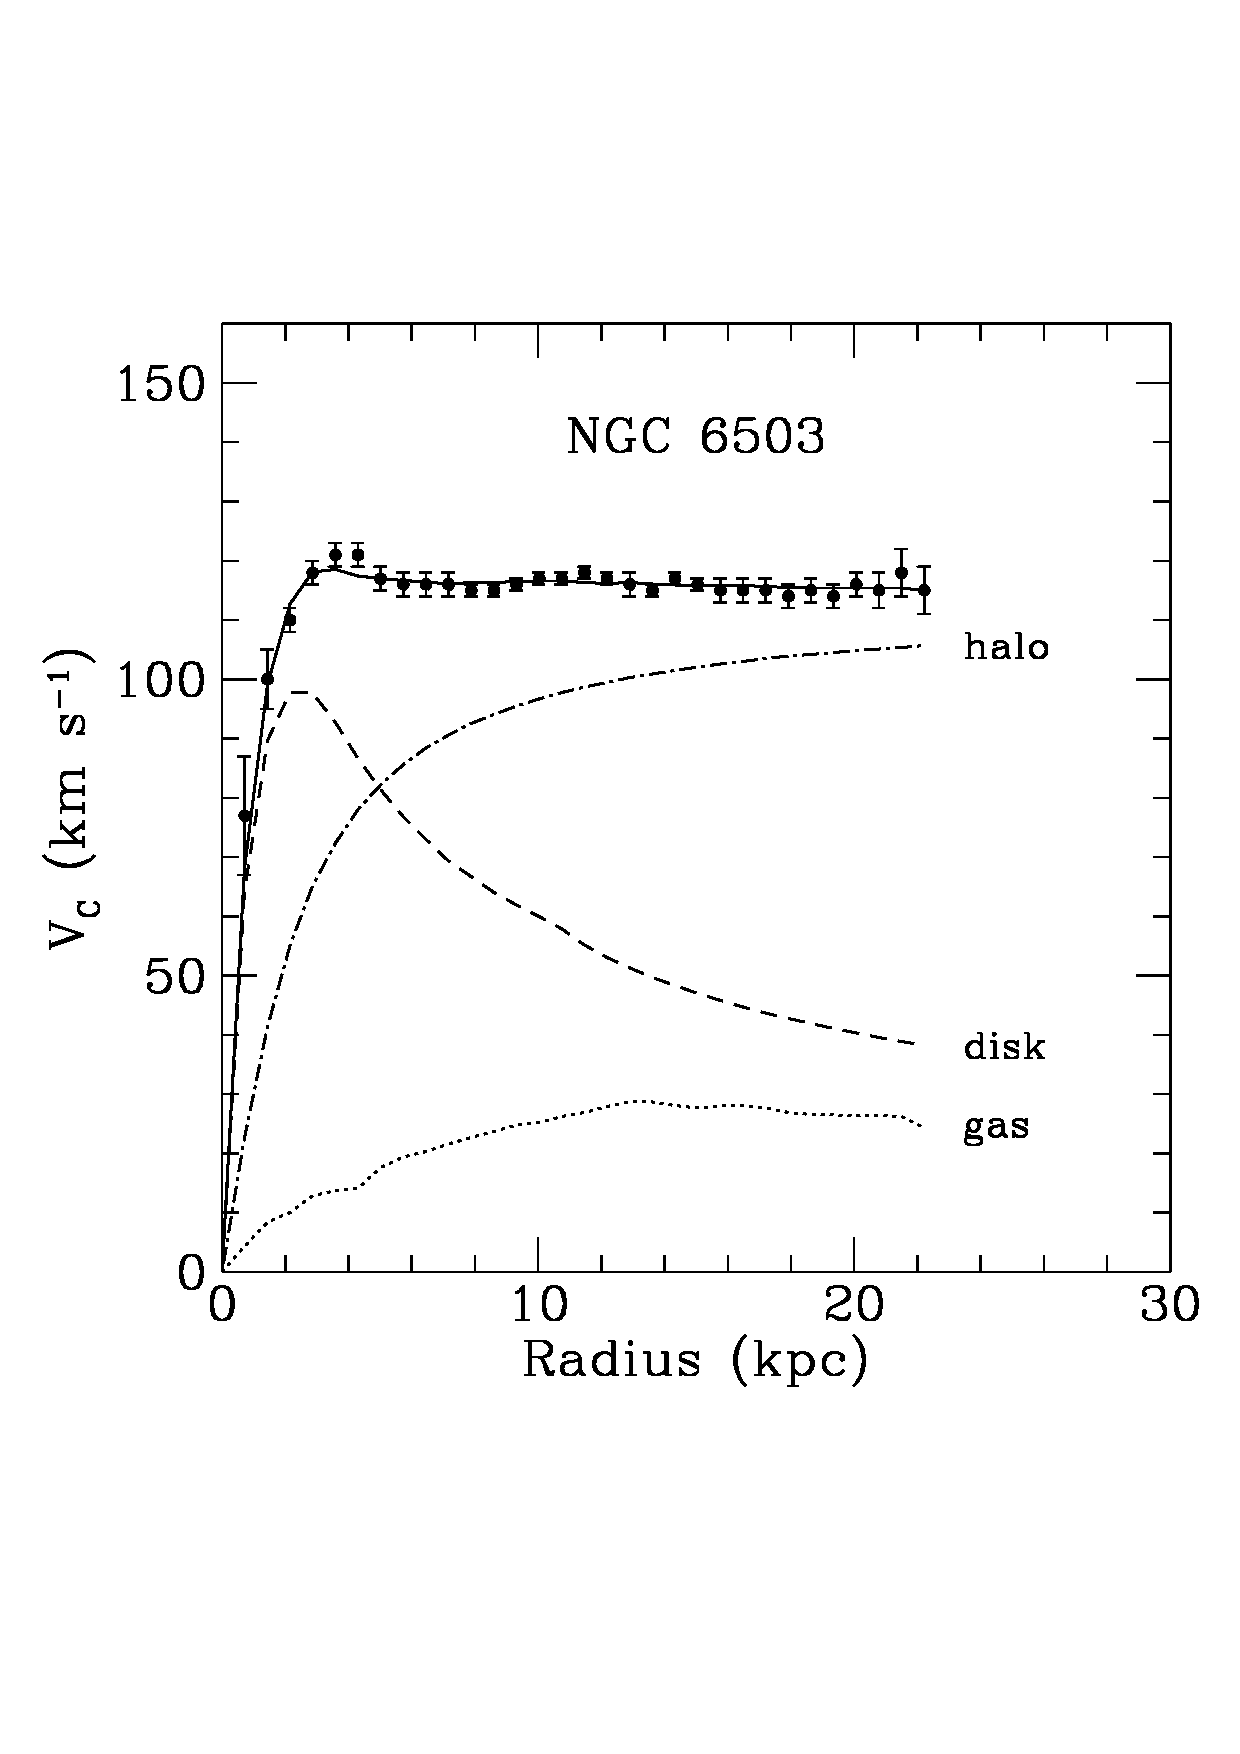
\includegraphics[width=0.4\textwidth]{imgs/Rotation}
    \caption{Rotation curve of the dwarf spiral galaxy NGC 6503 with the fitted halo, disc and gas distributions \cite{Begeman:1991iy}}
    \label{fg:RotationCurve}
\end{figure}
This rotation curve is shown in figure \ref{fg:RotationCurve} as an example. Newtonian circular orbits that should in this case at least be approximately obeyed demand 
\begin{equation}
v(r)=\sqrt{\frac{GM(r)}{r}}
\end{equation}
where $M(r)$ is the mass contained in a sphere of radius $r$ around the center of the galaxy. Without dark matter this is roughly constant beyond the optical disc such that the rotational velocity behaves like $v(r)\sim 1/\sqrt{r}$.
But the observation does not show this behaviour at all. Instead farther out the velocity becomes constant. This implies a halo of yet unaccounted mass with a density profile that falls off as $1/r^2$.

A better understanding of the distribution especially close to the center of this halo is an issue of ongoing research. \cite{Bertone:2004pz}

Another technique to deduce the distribution of mass in the universe that does not directly rely on the luminosity itself is gravitational lensing. Here a foreground galaxy or cluster bends space-time so that the light of a background object gets bend similar to an optical lens. Most impressive are constellations where the lensing object is circular and lines up with the background galaxy from the observers point of view. In this case the background galaxy gets distorted to a complete "Einstein ring", that appears with an angular "Einstein radius" 
\begin{equation}
\theta_E = \sqrt{\frac{4GM}{c^2}\frac{d_{LS}}{d_Ld_S}}
\end{equation}
where $M$ is the mass of the lensing object, $d_{LS}$ is the distance between the lens and source and $d_L (d_S)$ is the distance between the observer and the lens (source). Because the perfect alignment is rare, arcs rather than rings are observed. 
This fact was first used in the Abell 370 cluster to estimate the dark matter distribution and mass. One of the arcs used is shown in figure \ref{fg:abell}. 
\begin{figure}[ht]
  \centering
    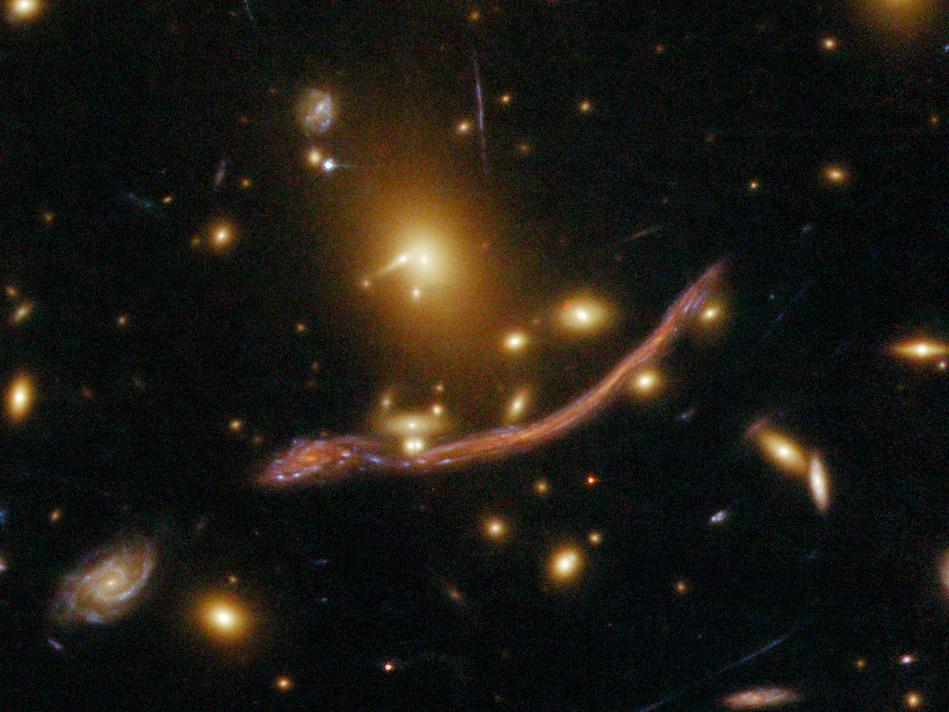
\includegraphics[width=0.4\textwidth]{imgs/large_web}
    \caption{Arc from gravitational lensing in Abell 370}
    \label{fg:abell}
\end{figure}
Comparing the necessary mass distribution for the lens and the optical distribution lead to two observations: Firstly again the luminous matter is far to light to account for the lensing and secondly the mass distribution also differs in position. 
This difference in position is most impressively shown in the bullet cluster shown in figure \ref{fg:bullet}. Here two clusters collided. During this collision the hot gas of both clusters interacted and is slowed. The dark matter component, lacking direct interaction is not slowed and continues largely its trajectory. This has also been used to falsify modified theories of gravitation. 
\begin{figure}[H]
  \centering
    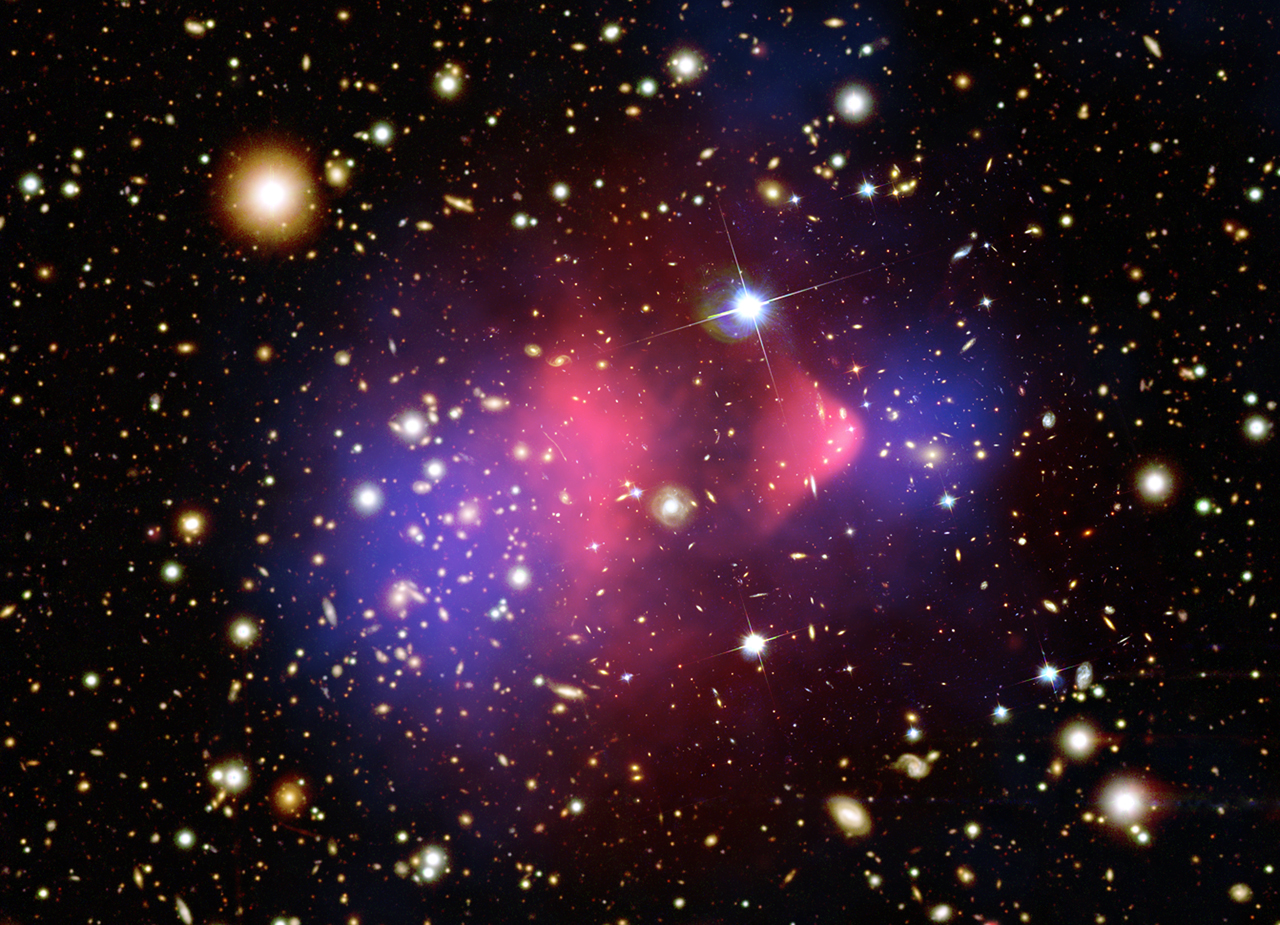
\includegraphics[width=0.4\textwidth]{imgs/bullet}
    \caption{Composite image of the galaxy cluster 1E 0657-556 with an X-ray image (red) and lensing mass distribution (blue) that do not coincide \cite{Massey:2010hh}}
    \label{fg:bullet}
\end{figure}

On much bigger scales the total amount of dark matter can be extracted from the Cosmic Microwave Background (CMB) in light of the recent survey by WMAP.
This has shown the CMB to be isotropic up to relative deviations of the order of $10^{-5}$. The remaining anisotropies can be used to constrain cosmological models.  Analysis of these distributions in the WMAP data results in
\begin{align}
\Omega_bh^2&=0.02264\pm0.00050\\
\Omega_Mh^2&=0.1364\pm0.0044
\end{align}
where $\Omega_b$ ($\Omega_M$) is the baryonic (matter) density relative to the critical density of the universe 
This further shows that the baryonic content is only responsible for a fraction of the entire matter content.


Since the large structure of the universe seems to strongly indicate the existence of dark matter, we still don't know what it is made of at the microscopic scale. All we know is that it interacts gravitationally but does not interact directly with light. 

The most strait forward remedy for this assumes dark matter to be made out of particles. Our job is then to develop models that at one hand explain the relic densities and on the other hand does not saturate existing bound of searches for new physics.

\section{Particle Dark Matter Candidates}
Dark matter candidates have to fulfil some conditions to be even worth considering. Since it should be present today, it either needs to be stable or its lifetime needs to be longer than the age of the Universe ($t_U=4\cdot 10^{17}s$).
Further it can't be electrically charged since it otherwise wouldn't be dark. And lastly it needs to reproduce the correct relic density
$\Omega_{DM}\sim 0.2$.
\paragraph{Axions}
Another interesting candidate is the the axion. 
Per se there is no reason for a CP-violating term to be absent in the theory. But the electric dipole moment of the neutron restricts \cite{Patrignani:2016xqp} an effective term like 
\begin{equation}
\mathcal{L}\supset -\Theta (\alpha_s/16\pi)F^{\mu\nu a}\epsilon_{\mu\nu\lambda\rho}F^{\lambda\rho a}
\end{equation}
to $|\Theta|\lesssim10^{-10}$. This can be explained by the introduction of the global Peccei-Quinn symmetry $U(1)_{PQ}$ that is subsequently spontaneously broken at the scale $f_A$. This cancels the aforementioned CP-violating term and introduces a pseudo Nambu-Goldstone boson -- the axion.
The axion-mass is then given by\cite{Bergstrom:2000pn}
\begin{equation}
m_A\approx 6\text{eV}\left(\frac{10^6\text{GeV}}{f_A}\right).
\end{equation}
The effective coupling constant of the axion to two photons is then proportional to $\alpha/f_A$. Thus the coupling and the mass of the axion can be simultaneously constrained.
Current bounds constrain the axion to be light ($\lesssim 10meV$). Even though the acceptable parameter strains gets smaller, there are still configurations where the axion might be the right dark matter candidate.

\paragraph{Neutrinos}
The standard model neutrinos are notoriously hard to detect and are already accounted for in the Standard Model. So at least that makes them seem to be good dark matter candidates. But since the total relic density can be estimated from the total mass of all three neutrino-generations to be $\Omega_\nu h^2 \lesssim 0.007$ , it will not suffice to account for all of the dark matter relic density.

\paragraph{SUSY}
To remedy the hierarchy problem of the Standard model one may introduce a new symmetry between bosons and fermions. Each particle has to have a super symmetric partner assigned that obeys the opposite statistics. If one extends the standard model to be super symmetric, the neutral $W$, $B$ and the neutral Higgs bosons (two different Higgs fields have to be introduced in SUSY) get fermionic superpartners that might mix to new mass eigenstates called neutralinos. To stop the proton from decaying, a new symmetry can be imposed -- the R-parity. If this is the case, the lightest of the neutralino will be stable and also serve as a dark matter candidate.

Since the super partners of neutrinos might acquire a large mass after SUSY-breaking these might also be seen as candidates. But the mass range that would result in the correct relic density is already ruled out by direct detection experiments searching for sneutrino-nucleon interactions.

\paragraph{Extra Dimensions}
Another somewhat different scenario are extra dimensions. There is no direct evidence, that the world we live in consists of more than three spacial and one temporal dimension. Nevertheless, extra dimensions are part of many beyond standard model theories. The idea that there might be more has received attention by Kaluza in his publication in 1921 that tried to unify gravity and electromagnetism in a five dimensional space-time so that Einstein's field equations yield general relativity and electromagnetism.
Modern QFT versions such as UED allow all fields to propagate in this extra dimension so that after compactification to for example a circle, their momentum-component gets quantised and result in so-called Kaluza-Klein states, that from the four dimensional point of view look like a tower of partner states with rising masses but same quantum numbers. A Kaluza-Klein-parity conservation then ensures, that the lightest state is stable and thus might serve as a dark matter candidate.
\newpage
\chapter{Leptophilic Dark Matter}
\label{ch:LepDM}
A particularly elegant way of avoiding direct detection bounds or explain why nothing has been found yet are leptophilic dark matter models where either the dark matter particles couple directly to the standard model leptons, or via another particle that mediates the interactions between dark matter and leptons. This completely avoids tree level interactions with gauge bosons and baryons that would lead to not-so-dark matter.

One way of incorporating these ideas is a hidden sector that contains only singlets under the standard model gauge group. Although this model on its own might explain the null results of direct detection efforts, this also paints the theoretically most boring picture. To connect the hidden sector to the standard model in a controlled manner, one may introduce additional fields, that mediate interactions between both sectors. These are then fittingly called portals. 

\section{Vector mediator}
The extension of the standard model by a new vector boson is well motivates both from a bottom up as well as from a top down perspective from grand unified theories. To this end the gauge group is extended by another $U_D(1)$ gauge group that is spontaneously broken such that the associated particles become massive. Such a particle is often labelled dark photon denoted by $A'$. This mediator couples additionally to the dark matter particles $\chi$. Since the exact nature of $\chi$ does not matter to this treatment it will be assumed to be a Dirac fermion for simplicity's sake.
The resulting Lagrangian can the be written as 
\begin{align*}
\mathcal{L}=& \mathcal{L}_\text{SM}-\frac{1}{4}F_{\mu\nu}'F'^{\mu\nu}+\frac{m_{A'}^2}{2}A_\mu'A'^\mu +\frac{\epsilon}{2}F_{\mu\nu}'F^{\mu\nu}-\sum_{l=e,\mu,\tau} e'_l\left(\bar{l}\gamma^\mu A'_\mu l+\bar{\nu}_l\gamma^\mu A'_\mu \nu_l\right)\\&+\bar{\chi}(i\slashed{\partial}-m_\chi)\chi -g_D\bar{\chi}\gamma^\mu A_\mu'\chi
\end{align*}
with the coupling constants $g_D$ and $e_l'$ left to be constrained and the kinetic mixing parameter $\epsilon$.
To avoid anomalies, one may chose to gauge any combination $X=yB-\sum x_iL_i$ of baryon number B and lepton family number $L_i$ that satisfy $3y=x_e+x_\mu+x_\tau$ \cite{Altmannshofer:2014pba}. Popular choices include gauged $B-L$ or $L_\mu-L_\tau$. While the former is highly constrained by direct collider searches and other 5th force experiments, the latter still exhibits rather weak constraints with a region that is even favoured by the $g_\mu -2$ anomaly.


\begin{figure}[H]
\centering
\begin{tikzpicture}
\begin{feynman}[layered layout]
\vertex (in){\(\gamma\)};
\vertex [right=of in](a);
\vertex [right=of a](b);
\vertex [right=of b](out){\(A'\)};
\diagram* {
(in)--[boson](a) -- [fermion,half left,edge label=\(f\)] (b) -- [fermion,half left] (a),
(b)--[boson](out)};
\end{feynman}
\end{tikzpicture}
\caption{Kinetic mixing of the SM-photon and the dark photon}
\label{fg:KinMix}
\end{figure}
The term proportional to $\epsilon$ has been added  to work with the most general renormalisable gauge invariant Lagrangian. 
Even though this term might be absent at tree level, as is the case for some GUT theories, it can be generated by loop contributions such as the diagram shown in figure \ref{fg:KinMix}, where the fermion running in the loop is charged both under the standard model and dark $U(1)$-group.
This leads to \cite{Rizzo:2018vlb}
\begin{equation}
\epsilon =\sum_l \frac{ee_l'}{12\pi^2}\ln\left(\frac{m_l^2}{\mu^2}\right)
\label{eq:KinMix}
\end{equation}
 and another effective interaction after diagonalization of the form 
\begin{equation}
\mathcal{L}\supset e\epsilon A'_\mu J_{em}^\mu
\end{equation}
such that now every electrically charged particle interacts with the dark photon as it is now millicharged under $U(1)_D$. This is used to put strong constraints on the parameter space.
This has also been used to explain the $g_\mu-2$ anomaly mentioned before. The discrepancy is removed with $m_{A'}<100\text{MeV}$ and $\epsilon\sim 10^{-3}$ for a kinetically mixed dark photon. But the last window of allowed parameter space has been closed by the NA48/2 Collaboration \cite{Goudzovski:2014rwa} such that there is no both problems cant be explained at once. 

If the A' is the lightest dark sector particle ($m_{A'}<2m_\chi$) it will mostly decay to the leptons $l$ it couples directly to with a the decay width
\begin{equation}
\Gamma(A' \rightarrow l^-l^+)=\frac{e_l^{'2}}{12\pi}m_{A'}\left(1+\frac{2m_l^2}{m_{A'}^2}\right)\sqrt{1-\frac{4m_l^2}{m_{A'}^2}}.
\end{equation}
This opens the scenario up to displaced vertex searches and other direct detection experiments. 

Once the decay to a $\chi$ pair is kinematically allowed ($m_{A'}>2m_\chi$) and $g_D > e'_l$ the mediator decays mainly invisibly with width 
\begin{equation}
\Gamma(A' \rightarrow \bar{\chi}\chi)=\frac{e_D^{2}}{12\pi}m_{A'}\left(1+\frac{2m_\chi^2}{m_{A'}^2}\right)\sqrt{1-\frac{4m_\chi^2}{m_{A'}^2}}
\end{equation}
such that direct detection is more difficult.  
When the dark photon only couples via kinetic mixing to the standard model the observed abundance is generated with \cite{Izaguirre:2014bca}
\begin{equation}
\alpha_D \equiv \frac{g_D^2}{4\pi} \approx 1.3\cdot 10^{-10}\left(\frac{m_{A'}}{10\text{MeV}}\right)^4\left(\frac{\text{MeV}}{m_\chi}\right)^2\frac{1}{\epsilon^2}.
\end{equation}
If $\epsilon$ is larger than this condition, $\Omega_\chi < \Omega_{\text{DM}}$ holds and $\chi$ might at most be a subdominant part of the total dark matter sector. 

Additional motivation for direct interactions with the muon specifically come from the $(g-2)_\mu$ discrepancy. The additional contribution from the vector is \cite{Kahn:2018cqs}:
\begin{equation}
\Delta a_\mu^V=\frac{e_\mu'^2}{4\pi^2}\int_0^1 d z \frac{m_\mu^2z(1-z)^2}{m_\mu^2(1-z)^2+m_{A'}^2z}
\end{equation}
which simplifies for $m_{A'}\ll m_\mu$ to
\begin{equation}
\Delta a_\mu^V \approx 1.6\times 10^{-9}\left(\frac{e_\mu'}{10^{-4}}\right)^2.
\end{equation}

\section{Scalar mediator}
Besides the vector mediator, a scalar might mediate interactions between the dark matter and the standard model. Besides the use as dark matter mediators, these models are proposed to solve the $(g-2)_\mu$ anomaly and the proton radius puzzle, depending on the coupled fermions. 
Here we propose a real scalar field $\phi$ with mass $m_\phi$ that is a singlet under the standard model gauge group and the same dark matter fermion $\chi$. The corresponding Lagrangian is 
\begin{align*}
\mathcal{L}=& \mathcal{L}_\text{SM}+\frac{1}{2}\partial_\mu \phi \partial^\mu \phi-\frac{m_{\phi}^2}{2}\phi^2 -\sum_{l=e,\mu,\tau} e'_l\bar{l} l \phi \\&+\bar{\chi}(i\slashed{\partial}-m_\chi)\chi -g_D\bar{\chi}\chi\phi.
\end{align*}
Obviously the introduction of the interaction term explicitly breaks the gauge invariance.
This might originate from a dimension 5 operator like 
\begin{equation}
\frac{c_l}{\Lambda}\phi \bar{L}_i\Phi e_{iR}+h.c.
\end{equation} 
where $\Phi$ is the standard model Higgs field that leads after SSB to the direct coupling of the scalar to the leptons with 
\begin{equation}
e'_l=\frac{c_l v}{\Lambda\sqrt{2}}.
\end{equation}
Most lepton-specific scalar mediator models considered in the literature propose the effective scalar couplings $c_l$ to be proportional to the Yukawa-coupling so that these follow the lepton mass hierarchy. 
A UV-completion above the scale $\Lambda$ will not be considered here but can be found for example as a Leptonic Higgs Portal in Ref\cite{Batell:2016ove}. Consequences besides the resulting low energy couplings are ignored for now.
This interaction leads  at one loop to an effective coupling to two photons of the form 
\begin{align*}
\frac{1}{4}g_{\gamma\gamma} \phi F_{\mu\nu} F^{\mu\nu}\\
\end{align*}
through the diagram shown in figure \ref{fg:PhotonCoupling}. The effective coupling strength $g_{\gamma\gamma}$ can be found in Ref. \cite{Chen:2018vkr}. This can be used to search for $\phi$ in the diphoton invariant mass distribution. 
The decay width to photons is
\begin{equation}
\Gamma(\phi\rightarrow \gamma \gamma)= \frac{\alpha^2m_\phi^3}{256\pi^3}\left\lvert\sum_{l=e,\mu,\tau} \frac{e'_l}{m_l}F_{1/2}(x_l,0) \right\lvert^2
\end{equation}
where $x_l = \frac{4m_l^2}{m_\phi^2}$ and and the loop function $F_{1/2}$ reads
\begin{equation}
F_{1/2}(x_l,0)= \begin{cases}
-2x_l\left[1+(1-x_l)\arcsin^2(x_l^{-1/2})\right]&x_l \geq 1\\
-2x_l\left[1-\frac{1-x_l}{4}\left(-i\pi +\log\frac{1+\sqrt{1-x_l}}{1-\sqrt{1-x_l}}\right)^2\right]&x_l<1
\end{cases}
\end{equation}

\begin{figure}[H]
\centering
\begin{tikzpicture}
\begin{feynman}[layered layout]
\vertex (in){\(\phi\)};
\vertex [right=of in](a);
\vertex [above right=of a](b);
\vertex [below right=of a](c);
\vertex [right=of b](f1){\(\gamma\)};
\vertex [right=of c](f2){\(\gamma\)};
\diagram* {
(in)--[scalar](a);
(a)--[fermion,edge label=\(l\)] (b) -- [fermion] (c) -- [fermion] (a);
(b)--[boson](f1);
(c)--[boson](f2)};
\end{feynman}
\end{tikzpicture}
\caption{One loop contribution to the $\phi$-photon coupling}
\label{fg:PhotonCoupling}
\end{figure}

For $g_D > e_l'$ and $2m_\chi < m_\phi$ the scalar mediator decays mostly invisibly to the dark sector.
The biggest decay width is then 
\begin{equation}
\Gamma(\phi \rightarrow \bar{\chi}\chi)=g_D^2\frac{m_\phi}{8\pi}\left(1-\frac{4m_\chi^2}{m_\phi}\right)^{3/2} .
\end{equation}
The main chance for collider experiments to constrain this model is then missing energy searches.
For $2m_\chi > m_\phi$ the mediator decays mostly visibly to the leptons it directly couples to as long as kinematically allowed.
\begin{equation}
\Gamma(\phi \rightarrow \bar{l}l)=e_l'^2\frac{m_\phi}{8\pi}\left(1-\frac{4m_l^2}{m_\phi}\right)^{3/2}
\end{equation}
This case behaves in collider experiments similar to the former if the scalar is long lived. If its short lived and decays at least in the majority of events in the detector material, it becomes accessible to displaced vertex or dilepton invariant mass searches.

This model has also been used to explain the $(g-2)_\mu$ results. This time its influence is slightly different:
\begin{equation}
\Delta a_\mu^S=\frac{e_\mu'^2}{16\pi^2}\int_0^1 d z \frac{m_\mu^2(1-z)(1-z^2)}{m_\mu^2(1-z)^2+m_{\phi}^2z}
\end{equation}
which simplifies for $m_{\phi}\ll m_\mu$ to
\begin{equation}
\Delta a_\mu^S \approx 6.0\times 10^{-10}\left(\frac{e_\mu'}{10^{-4}}\right)^2 .
\end{equation}
\newpage
\chapter{Experimental constraints}
\label{ch:ExConst}
There is a plethora of experimental searches for dark matter. Some of the applicable to the leptophilic models considered here will be presented in this section. 
\section{Four lepton Z decay}
The decay of the Z boson to four leptons has been studied with ATLAS detector at the LHC. 
\begin{figure}[H]
\centering
\begin{tikzpicture}
\begin{feynman}
\vertex (a) {\(\bar{q}\)};
\vertex [above right=1.41cm of a](c);
\vertex [above=2cm of a](b) {\(q\)};
\vertex [right=of c](d);
\vertex [below right=of d](e);
\vertex [above right=3cm of d](f1){\(l^-\)};
\vertex [below right=3cm of d](f4){\(l^+\)};
\vertex [above right=of e](g);
\vertex [above right= 1cm of g](f2){\(l^-\)};
\vertex [below right= 1cm of g](f3){\(l^+\)};

\diagram* {
(b) -- [fermion](c) -- [fermion] (a),
(c) -- [boson,edge label=\(Z/\gamma\)](d),
(f4) --[fermion](d) --[fermion](f1),
(f3) --[fermion](g) --[fermion](f2),
(e) --[boson,edge label=\(A'/Z/\gamma\)](g)
};
\end{feynman}
\end{tikzpicture}
\caption{Four lepton Z decay as a SM process (Z/$\gamma$) and BSM process (A')}
\label{fg:ZtoFourL}
\end{figure}
At the Z resonance, this process is dominated by the s-channel diagram shown in figure \ref{fg:ZtoFourL}.
This results in 
\begin{equation}
BR(\text{Z}\rightarrow 4l) = (3.20\pm 0.25 (\text{stat})\pm 0.13 (\text{syst}))\cdot 10^{-6}
\end{equation}
and is again consistent with the standard model \cite{Aad:2014wra}. This can be used to constrain the parameter space for new couplings. For example the Z' in the diagram shown above contibutes to the decay beyond the SM. But the techiques of the analysis only allow a narrow window of $5\text{ GeV} \lesssim m_{Z'}\lesssim 50 \text{ GeV}$ to be constrained \cite{Altmannshofer:2014pba}. This is mainly due to the cut on the dilepton invariant mass of $m_{l^+l^-}>5\text{ GeV}$.
\section{Neutrino trident production} 
Neutrino trident production is a process in which neutrinos are scattering of the coulomb field of the target material. The leading contributions come from a Photon coupling between the nucleus and the charged lepton and Z and W bosons coupling to the neutrino (see figure \ref{fg:trident}) and are thus suppressed. In addition, the destructive interference between diagrams with W and Z bosons suppress the SM process even further. 
\begin{figure}[H]
\centering
\begin{tikzpicture}
\begin{feynman}
\vertex (a1);
\vertex [above=0.2cm of a1](a2);
\vertex [above=0.2cm of a2](a3);
\vertex [right=3cm of a1](b1);
\vertex [right=3cm of a2](b2);
\vertex [right=3cm of a3](b3);
\vertex [right=3cm of b1](c1);
\vertex [right=3cm of b2](c2);
\vertex [right=3cm of b3](c3);
\vertex [above right=1.5cm of b3](d);

\vertex [above=0.5cm of d](e);


\vertex [above left=1.5cm of e](h1);
\vertex [left=3cm of h1](g1){\(\nu_\mu\)};
\vertex [right=3cm of h1](g2){\(\nu_\mu\)};
\vertex [above=0.5cm of c3](f1){\(\mu^-\)};
\vertex [below=0.5cm of g2](f2){\(\mu^+\)};;
\diagram* {
(a1) -- [fermion](b1) -- [fermion](c1),
(a2) -- [fermion](b2) -- [fermion](c2),
(a3) -- [fermion](b3) -- [fermion](c3),
(b3) -- [boson,edge label=\(\gamma\)](d),
(f2) --[fermion](e) -- [fermion](d) -- [fermion](f1),
(g1) -- [fermion](h1) -- [fermion](g2),
(e) -- [boson,edge label=\(Z/A'\)](h1)
};
\draw [decoration={brace}, decorate] (a1.south west) -- (a3.north west)
node [pos=0.5, left] {\(N\)};
\draw [decoration={brace}, decorate] (c3.south west) -- (c1.north west)
node [pos=0.5, right] {\(N\)};
\end{feynman}
\end{tikzpicture}
\caption{Neutrino-trident graph as a SM process (Z) and BSM process (A')}
\label{fg:trident}
\end{figure}
The CHARM-II collaboration and the CCFR collaboration both measured the crossection width a $\sim 20$ GeV beam on glass and $\sim 160$ GeV beam on an iron target respectively \cite{Altmannshofer:2014pba}.
The reported cross-sections relative to the SM-predictions are:
\begin{align*}
\frac{\sigma_\text{CHARM-II}}{\sigma_\text{SM}}&=1.58\pm 0.57\\
\frac{\sigma_\text{CCFR}}{\sigma_\text{SM}}&=0.82\pm0.28
\end{align*}
Bounds obtained for the cross section here can be used to obtain constraints on vectorial couplings to the muon and muon-neutrino for gauged $L_\mu-L_\tau$ or $L_e-L_\mu$ models. 
\section{Beam Dump Experiments}
One way to produce a vector mediator at a fixed target experiment is by the production of neutral pions or eta mesons  $p+p\rightarrow X+\pi^0/\eta$ that subsequently decays to $\pi^0/\eta\rightarrow A' + \gamma$ by the diagram shown in figure \ref{fg:BeamDumpPion}
\begin{figure}[H]
\centering
\begin{tikzpicture}
\begin{feynman}
\vertex (a1){\(\pi^0/\eta\)};
\vertex [right=2cm of a1](b);
\vertex [above right=2cm of b](c1);
\vertex [below right=2cm of b](c2);
\vertex [right=2cm of c1](f1){\(\gamma\)};
\vertex [right=2cm of c2](f2){\(A'\)};

\diagram* {
(a1) -- [scalar](b),
(b)--[fermion](c1)--[fermion](c2)--[fermion](b),
(c1)--[boson](f1),
(c2)--[boson](f2)
};
\end{feynman}
\end{tikzpicture}
\caption{Neutral meson decay to A' and $\gamma$ by kinetic mixing}
\label{fg:BeamDumpPion}
\end{figure}
The resulting branching ratio can then be related to that of the standard model radiative decay to two photons \cite{deNiverville:2011it}:
\begin{equation}
Br(\pi^0/\eta \rightarrow \gamma A')= 2\epsilon^2\left(1-\frac{m_{A'}^2}{m_{\pi/\eta}^2}\right)^3 Br(\pi^0/\eta \rightarrow \gamma\gamma)  .
\end{equation}
This can then be immediately be used to search for monophoton final states or simply missing energy.
Another way to use the resulting mediators is to utilise its decay products $\chi$ if the decay is allowed and rapid enough. The resulting $\chi$ beam can then be used to constrain the model by its scattering shown in the following diagram:
\begin{figure}[H]
\centering
\begin{tikzpicture}
\begin{feynman}
\vertex (a1);
\vertex [above=0.1cm of a1](a2);
\vertex [right=2cm of a1](b1);
\vertex [right=2cm of a2](b2);
\vertex [right=2cm of b1](c1);
\vertex [right=2cm of b2](c2){\(e/N\)};
\vertex [above=2cm of a2](a3){\(\chi\)};
\vertex [right=2cm of a3](b3);
\vertex [right=2cm of b3](c3){\(\chi\)};
 \node[above=1cm of b2, crossed dot] (d) {};


\diagram* {
(a1) -- [fermion](b1)--[fermion](c1),
(a2) -- [fermion](b2)--[fermion](c2),
(a3) -- [fermion](b3)--[fermion](c3),
(b2) --[boson,edge label=\(\gamma\)](d)--[boson,edge label=\(A'\)](b3)
};
\end{feynman}
\end{tikzpicture}
\caption{$\chi$ scattering on either electrons or nuclei.}
\label{fg:ChiScattering}
\end{figure}
These processes can be investigated with the data sets taken by the LSND and MiniBooNE experiments. Their data sets for the analysis of neutrino scattering can be used to constrain the parameter space, because the $\chi$-scattering leads to a similar signature. 
The case where the dark photon decays to an electron pair has been investigated by the NA48/2 experiment at CERN. Here an irreducible background comes from the standard model Dalitz decay. The resulting bounds on $\epsilon$ are shown in figure \ref{fg:NA48Bounds}.
\begin{figure}[H]
  \centering
    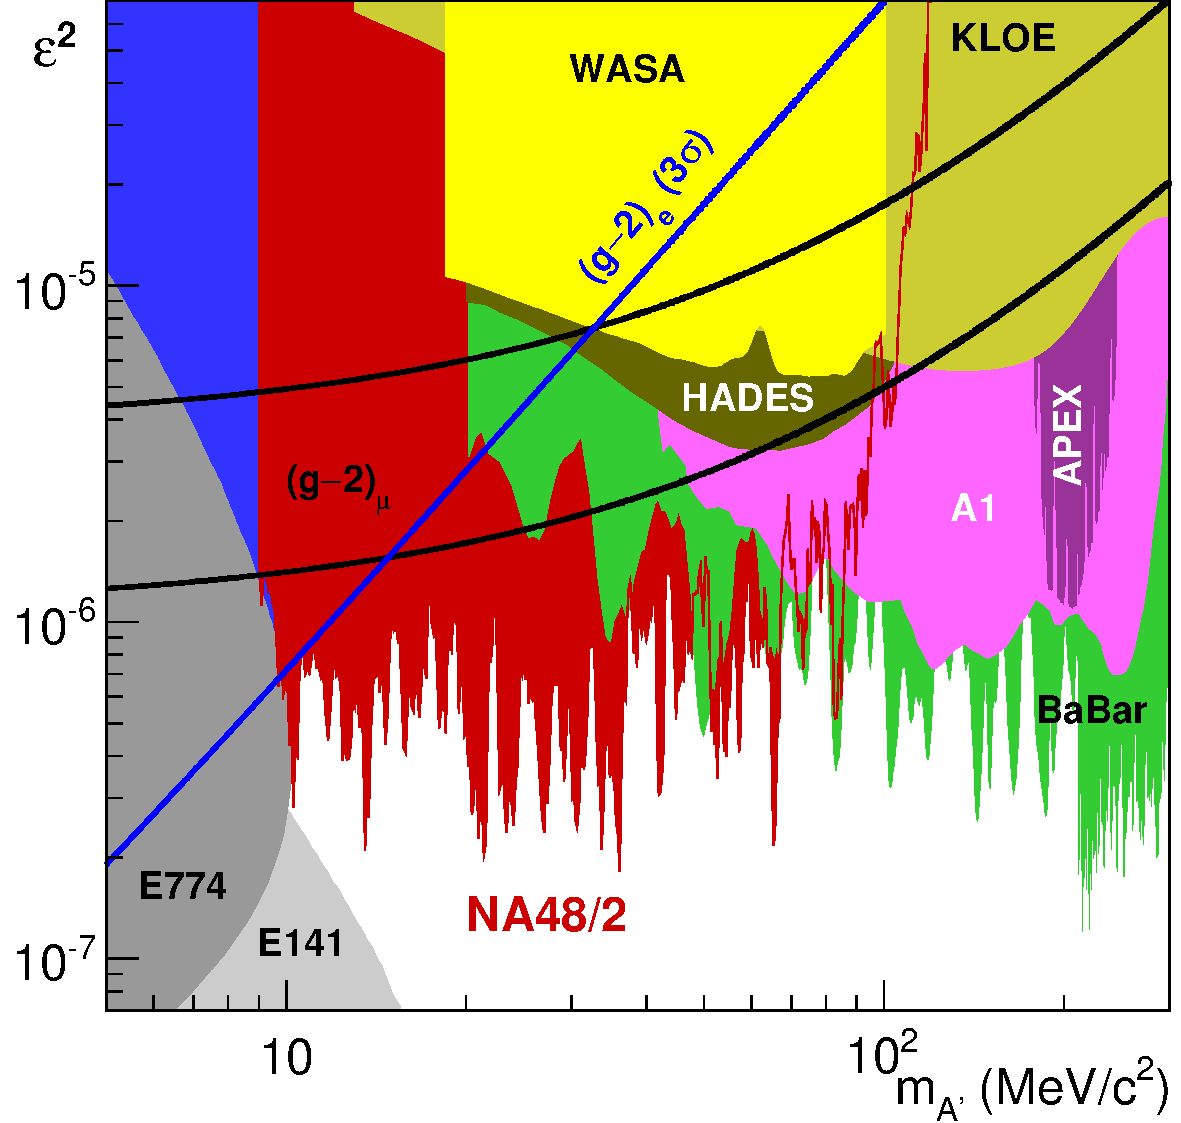
\includegraphics[width=0.4\textwidth]{imgs/dp_exclusion}
    \caption{Upper limits at 90\% CL on $\epsilon^2$ from \cite{Lurkin:2017aqo}}
    \label{fg:NA48Bounds}
\end{figure}
Although this result is only valid for pure kinetically mixed dark photons without the direct lepton coupling this can be used to construct the corresponding bound on $e'_l$ with the assumption that $\epsilon$ is absent at tree level by using equation \ref{eq:KinMix}.

\paragraph{NA64}
Another experiment that is used to constrain the dark photon models is NA64 at CERN SPS that dumps an electron beam on a target detector. Among the standard model particle shower, a dark photon might be created as bremsstrahlung shown in figure \ref{fg:DP-Porduction}. The possible detection is then by the large missing energy, that the dark photon carries away when it decays invisibly. The corresponding bound is shown in figure \ref{fg:BABAR}. The kinetic mixing parameter $\epsilon$ can in this case be identified with the direct electron coupling by $e_e'=e\epsilon$.

\begin{figure}[H]
\centering
\begin{tikzpicture}
\begin{feynman}
\vertex (a1);
\vertex [above=0.1cm of a1](a2);
\vertex [right=2cm of a1](b1);
\vertex [right=2cm of a2](b2);
\vertex [right=2cm of b1](c1);
\vertex [right=2cm of b2](c2){\(N\)};
\vertex [above=2cm of a2](a3){\(e\)};
\vertex [right=2cm of a3](b3);
\vertex [right=1.6cm of a3](c);
\vertex [right=2cm of b3](c3){\(e\)};
\vertex	[above=0.8cm of c3](f1){\(A'\)};


\diagram* {
(a1) -- [fermion](b1)--[fermion](c1),
(a2) -- [fermion](b2)--[fermion](c2),
(a3) -- [fermion](b3)--[fermion](c3),
(b2) --[boson,edge label=\(\gamma\)](b3),
(c) -- [boson](f1)
};
\end{feynman}
\end{tikzpicture}
\caption{Dark photon production as bremsstrahlung}
\label{fg:DP-Porduction}
\end{figure}
\section{\texorpdfstring{$e^+ e^-$}{e+e-} collider}
Another direct search for the dark photon has been carried out by the BABAR Collaboration. This experiment used collision data from the PEP-II B-factory and looked for events with one high energy photon with large missing momentum. This would receive a contribution from $e^+e^-\rightarrow \gamma A'$ where the dark photon decays invisibly to the dark sector. The collaboration established 90\% C.L. bounds on the mixing parameter of the kinetically mixed photon. Again this can straight forwardly be generalised to the model for the direct coupling to the leptons where $e_e'=e\epsilon$.
\begin{figure}[H]
  \centering
    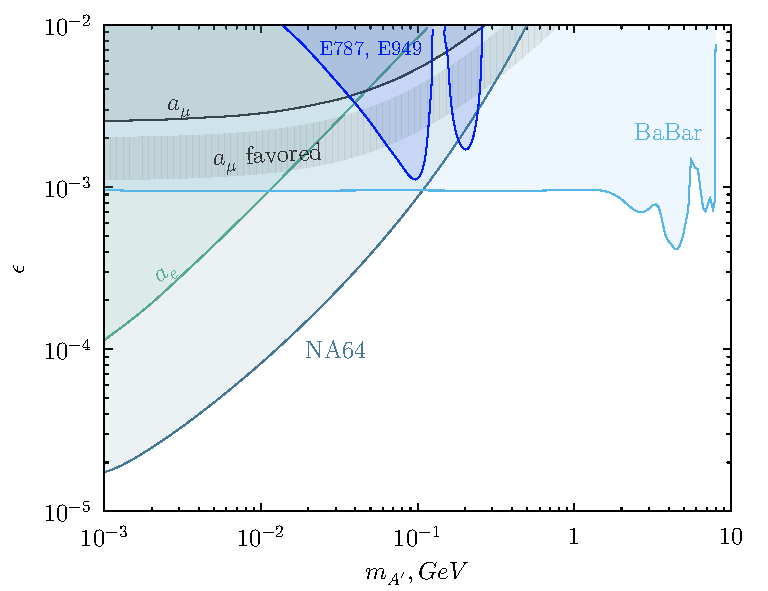
\includegraphics[width=0.6\textwidth]{imgs/exclusionInvisible-1909}
    \caption{BABAR and NA64 Upper limits at 90\% CL on $\epsilon$ from \cite{Banerjee:2018vgk}}
    \label{fg:BABAR}
\end{figure}
\section{Atomic Physics}
\paragraph{1S-2S transition in positronium}
Exotic atoms made of only leptons are a great place to test predictions from QED, because in contrast to hydrogen, the constituents are fundamental particles themselves. This avoids uncertainties like the internal structure of the proton in hydrogen, that affects the energy levels. 
If a new scalar field with mass $m_\phi$ that couples to particles i and j is introduced, it gives rise to a Yukawa potential of the form \cite{Frugiuele:2019drl}
\begin{equation}
V^{ij}(r)= -\frac{e'_i e'_j}{4\pi}\frac{e^{-m_\phi r}}{r}.
\end{equation}
This gives rise to energy shifts in atom like objects that contain particles i and j. The coupling to the electron on its own can be probed in bound states with multiple electrons that are at the same time well understood such as positronium and helium. For example the current standard model prediction and experimental measurement of the 1S-2S transition in positronium are:
\begin{align}
(E(2^3S_1)-E(1^3S_1))_{\text{Ps}}^\text{th}&=1233607222.13(58)\text{MHz}\\
(E(2^3S_1)-E(1^3S_1))_{\text{Ps}}^\text{exp}&=1233607216.4(3.2) \text{MHz}
\end{align}
The requirements that these deviate less than $2\sigma$ results in the bounds shown in figure \ref{fg:AtomicElectronBound}. Also included are bounds from the electron anomalous magnetic moment. This will be ignored in the further discussion because the contribution from two additional fields may cancel and render this bound deceiving. 

\begin{figure}[H]
\centering
\begin{subfigure}{.5\textwidth}
  \centering
  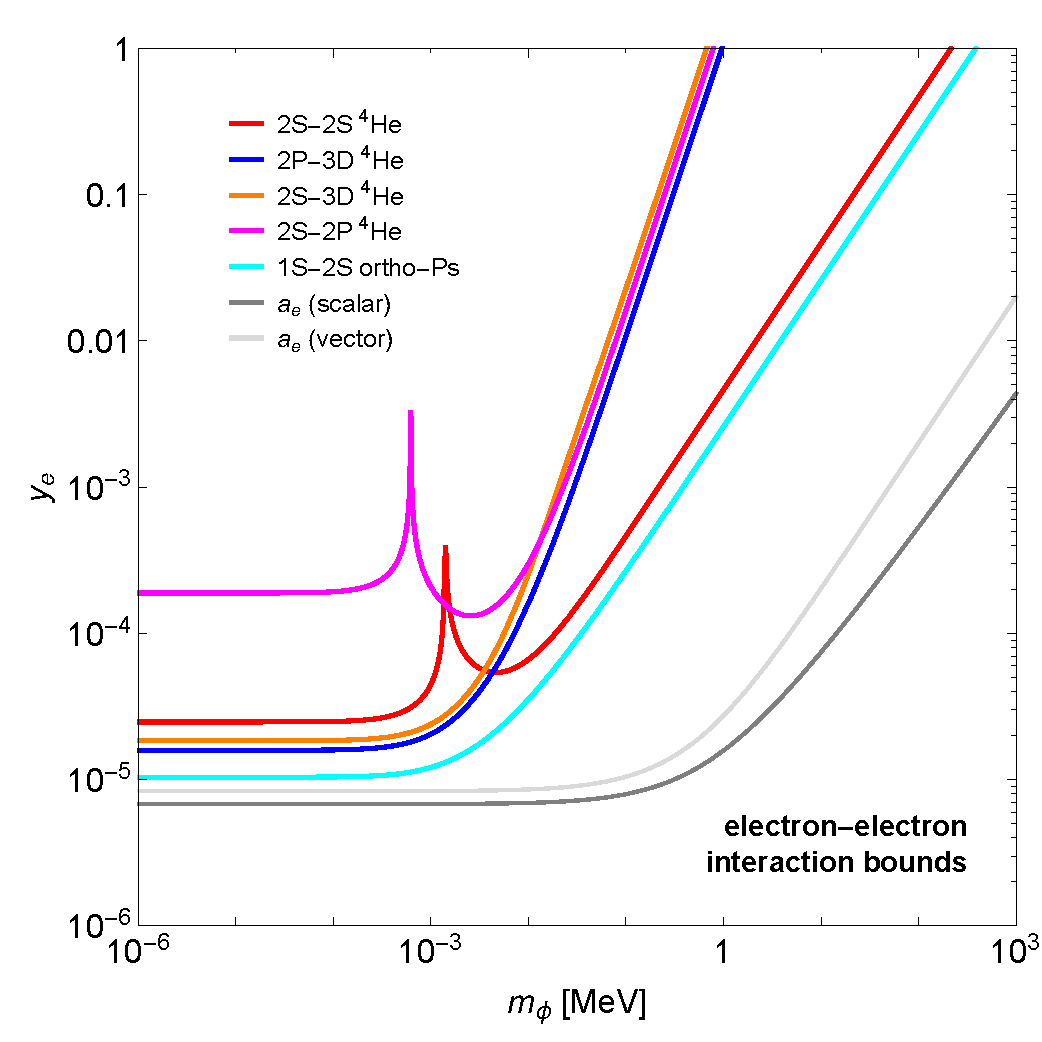
\includegraphics[width=\linewidth]{imgs/yebound-final}
  \caption{Upper limits on $y_e = e'_e$}
\end{subfigure}%
\begin{subfigure}{.5\textwidth}
  \centering
  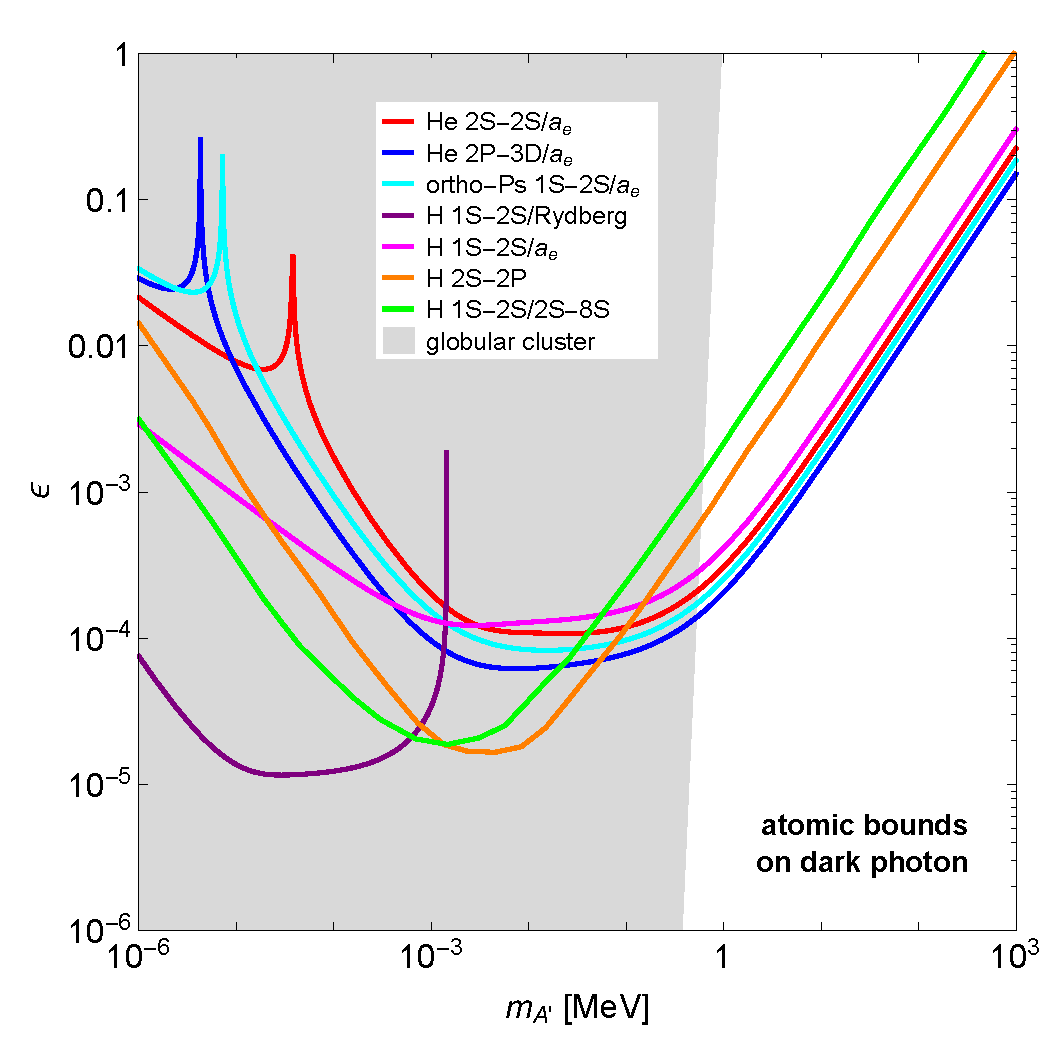
\includegraphics[width=\linewidth]{imgs/DP-final}
  \caption{Upper limits on $\epsilon$}
\end{subfigure}
\caption{Taken from \cite{Delaunay:2017dku} }
\label{fg:AtomicElectronBound}
\end{figure}

\paragraph{Muonium}
The other coupling relevant to this work is to the muon. Sadly the direct analogue to the previous paragraph consisting of only muons, the true muonium has neither been measured nor even been seen. The alternative is the spectrum of muonium, that is despite of its name a bound state of an electron and an anti-muon. The theoretical and experimental values for the 1S-2S transitions for this case are:
\begin{align}
(E(2S_1)-E(1S_1))_{\text{Mu}}^\text{th}&=2455528941.0(9.8)\text{MHz}\\
(E(2S_1)-E(1S_1))_{\text{Mu}}^\text{exp}&=2455528935.8(1.4) \text{MHz}.
\end{align}
Special care has to be taken to evaluate the theoretical value, because the 1S-2S transition is used to calculate $m_\mu/m_e$ which in turn sets the muon mass, so it's not independent on the BSM influence. 
Also the lamb shift in muonium has been calculated and measured to :
\begin{align*}
(E(2S_{1/2})-E(2P_{1/2})_\text{Mu}^\text{th}&=1047.284(2)\text{MHz}\\
(E(2S_{1/2})-E(2P_{1/2})_\text{Mu}^\text{exp}&=1042(22)\text{MHz}
\end{align*}
Both can seperately be used to construct bound on the product of couplings $e'_\mu e'_e=g_e\times g_\mu$ \cite{Frugiuele:2019drl} These are shown in figure \ref{fg:MuoniumBounds}
\begin{figure}[H]
  \centering
    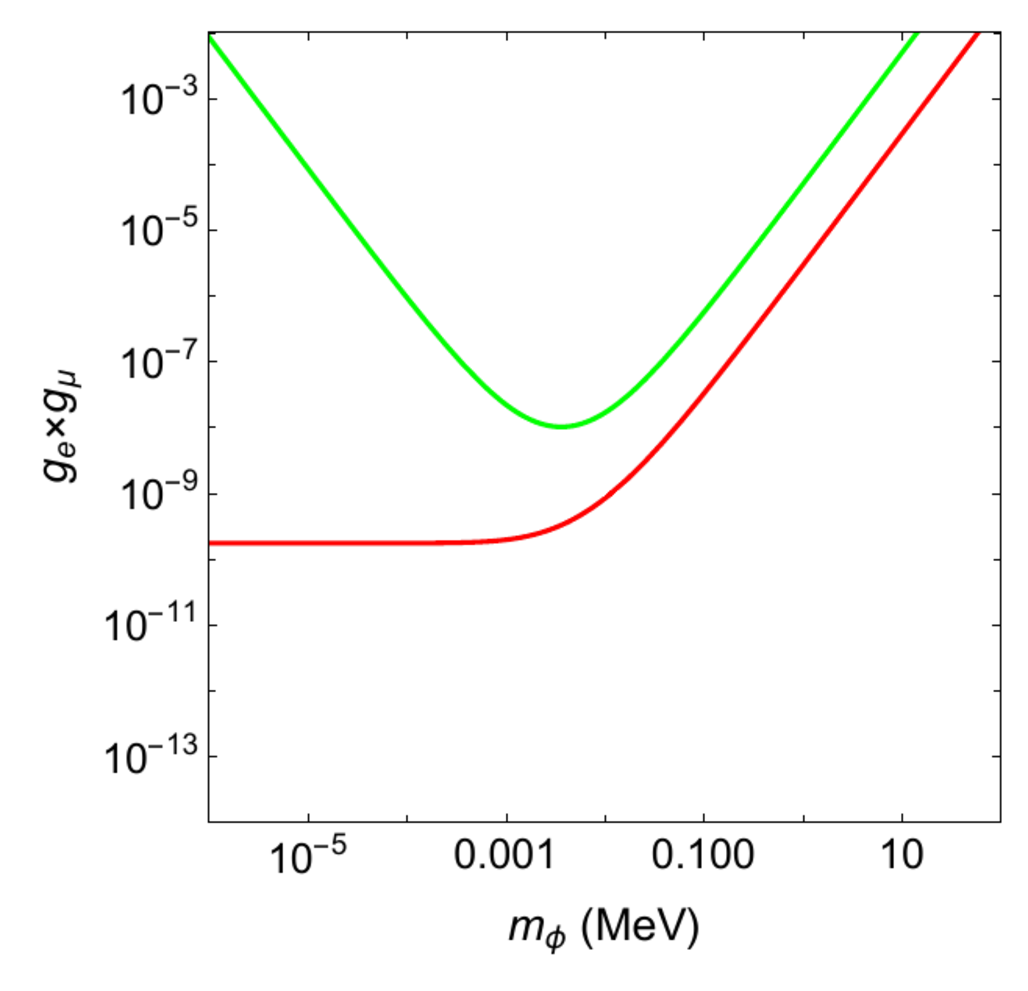
\includegraphics[width=0.5\textwidth]{imgs/muonium1}
    \caption{Upper limits at 95\% CL on $g_e\times g_\mu$ from Mu 1S-2S transition (red) and the Lamb shift (green). Taken from \cite{Frugiuele:2019drl}}
    \label{fg:MuoniumBounds}
\end{figure}
\section{Future Experiments}
\paragraph{Belle II}
Belle II is an experiment at the SuperKEKB $e^+e^-$collider in Japan that started data acquisition in early 2018. Even though its main use is as a B-factory to study B-meson properties, it will also serve as a test ground for electrophilic new physics. Its data set will allow stronger constraints to the electron dark photon coupling in mono photon events with a photon energy of $E_\gamma = \frac{s-M_{A'}^2}{2\sqrt{s}}$ when the dark photon is produces on shell and escapes the detector/ decays to the dark sector, or additionally with two opposite leptons with a center of mass energy of the dark photon mass when it decays to the standard model leptons. 
In either case the bounds on the kinetic mixing parameter can be straight forwardly be converted to the direct lepton coupling models. To reach higher sensitivity for these events, the upgrade from Belle to Belle II included a single photon trigger ans is going to run at a higher luminosity.\cite{Inguglia:2016acz}.  
\paragraph{NA64-\texorpdfstring{$\mu$}{mu}}
Since the NA64-experiment is run only with electrons and only searches for dark photon decays to an $e^+e^-$ pair, its insensitive to any coupling to muons. To remedy this and explore the $(g-2)_\mu$ anomaly further, the $NA64_\mu$-run is proposed and if its approved is scheduled to run after 2021. Here a $\mu^+$-beam on target is used to search for an excess of missing momentum events where the muon is slightly scattered that points to the bremsstrahlung production of a mediator with subsequent invisible decay. Among the gauged $L_\mu-L_\tau$ this might be most useful for scalar mediators coupling to muons.
\paragraph{$M^3$: Muon Missing Momentum Experiment}
$M^3$ is a proposed experiment at Fermilab where a $\SI{15}{\giga \eV}$ muon beam impacts an active target. Then signatures for $\mu N \rightarrow \mu N \slashed{E}$ are searched. In this case the missing energy $\slashed{E}$ comes from the invisible decay of the mediator coupled to the muon that is produced by bremsstrahlung. In phase 1 this is then proposed to deliver bounds on the scalar coupling of $<3\dot10^{-4}$ and on the vector coupling of  $<2\dot10^{-4}$ for masses below $\SI{100}{\mega \eV}$ \cite{Kahn:2018cqs}.
\newpage
\newpage
%\section{Model}

%\newpage
\chapter{Standard Model Muon decay}
\label{ch:SMMuon}
The muon exhibits only three standard model decay modes, namely $\mu^-\rightarrow e^-\bar{\nu}_e\nu_\mu$, the corresponding radiative mode $\mu^-\rightarrow e^-\bar{\nu}_e\nu_\mu\gamma$ and $\mu^-\rightarrow e^-\bar{\nu}_e\nu_\mu e^+e^-$. The former is seen in almost every muon decay, while the last two combined are responsible for less than one in every 10.000 decays so its justified to assume the muon has only one decay mode. This clean background and the straightforward production and detection render the muon decay a great proving ground for the weak interaction. This can be turned around to set Fermis coupling constant by matching it to the muon lifetime.
Even though being investigated there is no sign of other decay modes beyond the standard model that would point to new physics. 
\begin{figure}[H]
\centering
\begin{tikzpicture}
\begin{feynman}
\vertex (a) {\(\mu^{-}\)};
\vertex [right=of a] (b);
\vertex [above right=of b] (f1){\(\nu_\mu \)};
\vertex [below right=of b] (c);
\vertex [above right=of c] (f2){\(e^-\)};
\vertex [below right=of c] (f3){\(\bar{\nu}_e\)};
\diagram* {
(a)--[fermion](b)--[fermion](f1),
(b)--[boson, edge label'=\(W\)](c),
(f2)--[anti fermion](c)--[anti fermion](f3)};
\end{feynman}
\end{tikzpicture}
\caption{Standard model muon decay mediated by the V-A interaction}
\label{fg:SM-Muondecay}
\end{figure}
The decay is mediated by the charged current interaction as shown in diagram \ref{fg:SM-Muondecay}. New physics might alter the V-A structure such that the angular distribution of the electrons momentum relative to the polarisation of the muon is sensitive to deviations from the standard model.  

To this end its important to understand the standard model induced structure of the decay. Assigning momenta $P,P_{\nu_\mu},P_e,P_{\nu_e}$ and polarisations $s,s_{\nu_\mu},s_e,s_{\nu_e}$ to the $\mu^-,\nu_\mu,e^-$ and $\bar{\nu}_e$ respectively
 and neglecting the momentum transfer in the W-propagator the corresponding matrix element is
 \begin{equation}
 -i\mathcal{M}=\frac{-ig^2}{8m_W^2}\bar{u}(P_{\nu_\mu},s_{\nu_\mu}) \gamma_\mu(1-\gamma^5)u(P,s)\bar{u}(P_e,s_e)\gamma^\mu(1-\gamma^5)v(P_{\nu_e},s_{\nu_e}).
 \end{equation}
In the squared matrix element there will be a term proportional to $u(P,s)\bar{u}(P,s)$ that is replaced by 
\begin{equation}
u(P,s)\bar{u}(P,s)=(\slashed{P}+m_\mu)\frac{1+\gamma^5\slashed{S}}{2}
\end{equation}
where $\slashed{S}$ contains the spin four-vector of the muon.
Summing over the final state polarisations since its not measured this results in
\begin{equation}
|\mathcal{M}|^2=\frac{2g^4}{M_w^4} (P_{\nu_\mu} \cdot P_e ) (P-m_\mu S)\cdot P_{\nu_e}.
\end{equation}
All that is left is the phase space integration
\begin{equation}
d\Gamma = \frac{1}{2m_\mu}\frac{1}{2E_e}\frac{d^3p_e}{(2\pi)^2}\frac{1}{2E_{\nu_e}}\frac{d^3p_{\nu_e}}{(2\pi)^2}\frac{1}{2E_{\nu_\mu}}\frac{d^3p_{\nu_\mu}}{(2\pi)^2}|\mathcal{M}|^2(2\pi)^4\delta^{(4)}(P-P_e-P_{\nu_\mu}-P_{\nu_e})
\end{equation}
 while leaving out the integral over the electrons energy and the angle $\theta$ between the electron momentum and the muon spin to get the decay spectrum. 
This is written with the new variable $x=2E_e/m_\mu$ as the electron energy normalised to the maximum value and the Fermi coupling $G_f=g^2/(4\sqrt{2}m_W^2)$ as
\begin{align}
\frac{d^2\Gamma}{dxd\cos\theta}=\frac{G_f^2m_\mu^5}{192\pi^3}\left[x^2\left((3-2x)+(1-2x)\cos\theta\right)\right]
\label{eq:DiffrateSimple}
\end{align}
where the term outside the square brackets is the total decay width.
\begin{figure}[H]
  \centering
    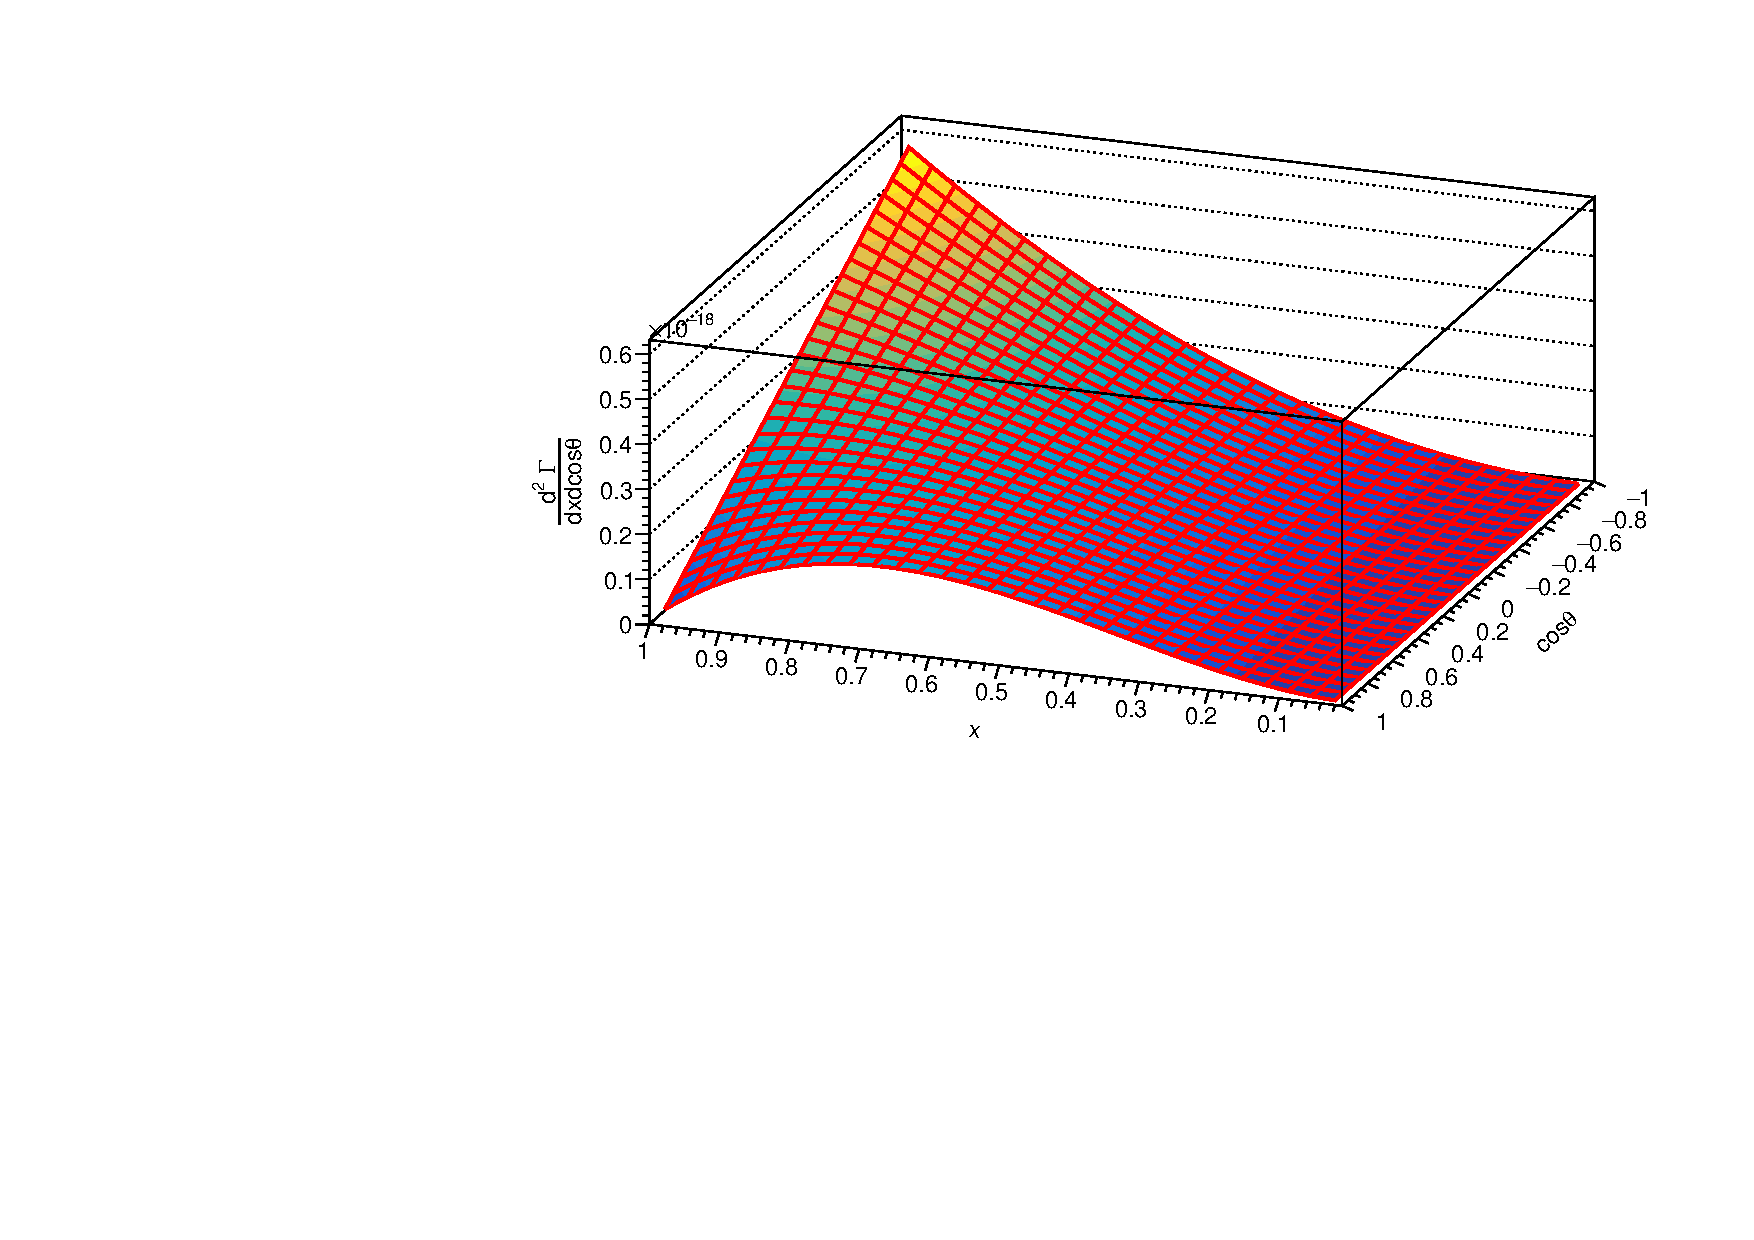
\includegraphics[width=0.8\textwidth]{imgs/MuonSpectrum}
    \caption{Standard model muon decay spectrum}
    \label{fg:SM-MuonSpectrum}
\end{figure}
The corresponding spectrum is shown in figure \ref{fg:SM-MuonSpectrum}.
If one were not to neglect the electron mass the calculation gets a bit more messy, but leads to the more precise result
\begin{equation}
\frac{d^2\Gamma}{dxd\cos\theta}=\frac{m_\mu}{4\pi^3} W_{e\mu}^4G_f^2\sqrt{x^2-x_0^2}\left(F_{\text{IS}}(x)-P_\mu\cos\theta F_{\text{AS}}(x)\right)
\label{eq:Diffrate}
\end{equation}
 with $W_{e\mu}$ as the maximum electron energy $(m_\mu^2+m_e^2)/2m_\mu$, $x_0$ the minimum electron energy $m_e/W_{e\mu}$, $P_\mu$ the degree of muon polarisation and the functions for the isotropic part $F_\text{IS}(x)$ and the anisotropic part $F_\text{AS}(x)$ given below \cite{Patrignani:2016xqp}.
\begin{align*}
F_\text{IS}&=x(1-x)+\frac{2}{9}\rho(4x^2-3x-x_0^2)+\eta x_0(1-x)\\
F_\text{AS}&=\frac{1}{3}\xi\sqrt{x^2-x_0^2}\left[1-x+\frac{2}{3}\delta(4x-4+\sqrt{1-x_0^2}\right]
\end{align*} 
Here the Michel parameters $\rho,\eta,\xi$ and $\delta$ have been introduced. The corresponding standard model values can be found by comparison of coefficients between equation \ref{eq:DiffrateSimple} and \ref{eq:Diffrate} and are $3/4$, $0$, $1$ and  $3/4$ respectively.
These can also be used to parametrise additional contributions to the muon decay that can be expressed as an effective four point interaction. These matrix elements can then be written as \cite{Patrignani:2016xqp}:
\begin{equation}
\frac{4G_f}{\sqrt{2}}\sum_{\substack{\gamma=\text{S,V,T}\\\epsilon,\mu = \text{R,L}}}g_{\epsilon\mu}^\gamma \langle\bar{e}_\epsilon \lvert \Gamma^\gamma \lvert (\nu_e)_n \rangle\langle (\bar{\nu}_\mu)_m \lvert \Gamma_\gamma \lvert \mu_\mu \rangle
\end{equation}
where the indices S,V,T denote scalar, vector and tensor interactions respectively while $\Gamma$ represents the corresponding operators and the R/L indices indicate the chirality of the fermions.
The amplitudes $g_{\epsilon\mu}^\gamma$ can then be combined to 
\begin{align*}
a&= 16( \lvert g_\text{RL}^V \lvert ^2 + \lvert g_\text{LR}^V \lvert ^2)+ \lvert g_\text{RL}^S + 6g_\text{RL}^T \lvert ^2+ \lvert g_\text{LR}^S + 6g_\text{LR}^T \lvert ^2  \\
a'&=16( \lvert g_\text{RL}^V \lvert ^2 - \lvert g_\text{LR}^V \lvert ^2)+ \lvert g_\text{RL}^S + 6g_\text{RL}^T \lvert ^2- \lvert g_\text{LR}^S + 6g_\text{LR}^T \lvert ^2 \\
b&=4(\lvert g_\text{RR}^V \lvert^2+\lvert g_\text{LL}^V \lvert ^2)+\lvert g_\text{RR}^S \lvert ^2+\lvert g_\text{LL}^S \lvert ^2\\
b'&=4(\lvert g_\text{RR}^V \lvert^2-\lvert g_\text{LL}^V \lvert ^2)+\lvert g_\text{RR}^S \lvert ^2-\lvert g_\text{LL}^S \lvert ^2\\
c&=\frac{1}{2}(\lvert g_\text{RL}^S -2g_\text{RL}^T \lvert ^2+\lvert g_\text{LR}^S -2g_\text{LR}^T \lvert ^2)\\
c'&=\frac{1}{2}(\lvert g_\text{RL}^S -2g_\text{RL}^T \lvert ^2-\lvert g_\text{LR}^S -2g_\text{LR}^T \lvert ^2)\\
\alpha &= 8\Re (g_\text{RL}^V(g_\text{LR}^{S*}+6g_\text{LR}^{T*})+g_\text{LR}^V(g_\text{RL}^{S*}+6g_\text{RL}^{T*}))\\
\beta &=-4\Re (g_\text{RR}^V g_\text{LL}^{S*}+g_\text{LL}^V g_\text{RR}^{S*})
\end{align*}
which is a parametrisation that has also been experimentally measured. In terms of these the Michel parameters are given by:
\begin{align}
\rho -\frac{3}{4}&= \frac{3}{4}\frac{2c -a }{a+4b+6c}\\
\eta &=\frac{\alpha -2\beta}{a+4b+6c}\\
\delta -\frac{3}{4}&=\frac{9}{4}\frac{2c'-a'}{3a'+4b'-14c'}\\
1-\xi\frac{\delta}{\rho}&=\frac{b+b'+2(c-c')}{b+2c}
\end{align}
The standard model alone leads to all amplitudes to vanish except $g_{LL}^V =1$.
 
\paragraph{Experimental test}
The most recent and precise measurement of the Michel parameters $\rho$, $\delta$ and $P_\mu\xi$ has been done by the TWIST Collaboration \cite{TWIST:2011aa}. The experiment used the proton beam at TRIUMF accelerator in Vancouver. The protons were dumped on a carbon target, creating pions of which some decay in the material via the two body decay shown in chapter \ref{ch:SM-PionDecay}. These at the time 100\% polarised muons are then stopped at a silver or aluminium foil-target in the TWIST detector. In the time between the creation and decay the muons depolarise. This has to be corrected in the analysis. Then the momentum-angle distribution of the resulting positrons was measured. The analysis was done blind. Decay parameters were chosen randomly close to the expected values before the analysis and the corresponding Monte Carlo spectrum $S_\text{MC}$ including radiative corrections with a detector simulation was generated while the chosen parameters are kept hidden to avoid any human bias. The analysis is then done to extract $\Delta\rho$, $\Delta (P_\mu \xi)$ and $\Delta( P_\mu\xi\delta)$ from
\begin{equation}
S_\text{Data}=S_\text{MC}+\frac{\partial S}{\partial\rho}\Delta \rho+\frac{\partial S}{\partial P_\mu\xi}\Delta(P_\mu\xi)+\frac{\partial S}{\partial P_\mu \xi \delta}\Delta(P_\mu\xi\delta)
\end{equation}
After these parameters were extracted and the uncertainties were determined the hidden parameters can be revealed and the full result calculated. 
The results are :
\begin{align*}
\rho &= 0.74977\pm0.00012(\text{stat.})\pm 0.00023(\text{sys.})\\
\delta &=0.75049\pm0.00021(\text{stat.})\pm 0.00027(\text{syst.})\\
P^\pi_\mu\xi\delta/\rho&=1.00170^{+0.00156}_{-0.00071}
\end{align*}

Including these results, a global analysis results in 
\begin{align*}
\rho &=0.74979 \pm 0.00026\\
\eta &=0.057 \pm 0.034\\
\delta &= 0.75047\pm 0.00034\\
\xi &= 1.0009^{+0.0016}_{-0.0007}
\end{align*}
and is used for the following constraining of the dark matter mediators.
\newpage
\chapter{Bounds from \texorpdfstring{$\mu^-$}{muon} decays}
\label{ch:MuBounds}
As was shown in the previous section, Michel parameters are linear combinations of coupling strengths of effective four point interactions that lead to the muon decay. Any three body decay that has a valid representation as this effective coupling then be calculated and expressed as a deviation from the known standard model values. This has long been used to restrict any additional interaction that might contribute to the decay. 

One path that has not been investigated beyond the change in the decay width however is the influence of another four body decay of the muon besides the radiative decay. If the muon decays to $e^-\bar{\nu}_e \nu_\mu X$ where $X$ is either a scalar $\phi$ or a dark photon $A'$, this would alter the decay spectrum but still register as a three body decay, as long as $X$ leaves the detector undetected or decays invisibly. The obvious standard model background is the radiative decay, where the photon is not detected. This nevertheless will alter the experimentally taken spectrum and in turn the determined Michel parameters. As an example this is shown in figure \ref{fg:MuonBSMContribution} where the dark photon couples to the electron and electron neutrino.
\begin{figure}[ht]
\centering
\begin{subfigure}{.5\textwidth}
  \begin{tikzpicture}
\begin{feynman}
\vertex (a) {\(\mu^{-}\)};
\vertex [right=of a] (b);
\vertex [above right=of b] (f1){\(\nu_\mu \)};
\vertex [below right=of b] (c);
\vertex [above right=of c] (d);
\vertex [above right=of d] (f2){\(e^-\)};
\vertex [below right=of d] (f4){\(A'\)};
\vertex [below right=of c] (f3){\(\bar{\nu}_e\)};
\diagram* {
(a)--[fermion](b)--[fermion](f1),
(b)--[boson, edge label'=\(W\)](c),
(d)--[boson](f4),
(f2)--[anti fermion](d)--[anti fermion](c)--[anti fermion](f3)};
\end{feynman}
\end{tikzpicture}
\end{subfigure}%
\begin{subfigure}{.5\textwidth}
\begin{tikzpicture}
\begin{feynman}
\vertex (a) {\(\mu^{-}\)};
\vertex [right=of a] (b);
\vertex [above right=of b] (f1){\(\nu_\mu \)};
\vertex [below right=of b] (c);
\vertex [above right=of c] (f2){\(e^-\)};
\vertex [below right=of c] (d);
\vertex [above right=of d] (f4){\(A'\)};
\vertex [below right=of d] (f3){\(\bar{\nu}_e\)};
\diagram* {
(a)--[fermion](b)--[fermion](f1),
(b)--[boson, edge label'=\(W\)](c),
(d)--[boson](f4),
(f2)--[anti fermion](c)--[anti fermion](d)--[anti fermion](f3)};
\end{feynman}
\end{tikzpicture}
\end{subfigure}
\caption{Example diagrams that result from a coupling between the dark photon and the electron/electron neutrino }
\label{fg:MuonBSMContribution}
\end{figure}
Since this cant be expressed as a four point interaction, there is not simple expression for the altered parameters. Another fact, that complicate things is there not much hope for a analytical solution for the phase space integral. So a numerical integration procedure is needed. 
\section{Calculation of the spectrum}
This case is less restricted than the pion decay, because here we deal with both electrons and muons.
The models that are investigated are a scalar coupling to the electron, the muon and both at the same time. The spin 1 model will couple to both the charged leptons as well as the neutrinos. For this case the coupling to the electron and muon are separately tested as well as combined. Additionally to this also the coupling to the left and right chiral fields are probed independently. 
The experimental values were obtained with $\sim 3\cdot 10^{9}$ muons. If one were to probe the BSM-models with Monte-Carlo event generators one would need BSM events of the order of $10^7$ to reach comparable or even better sensitivity and to be able to probe large coupling constants.
This takes long and generated a huge amount of data because even at later stages ignored information is generated and stored. 
This is why a custom numerical integration method was used. 

The squared matrix element for the polarised decay was traced and simplified in \textsc{Mathematica} by using the \textsc{Feyncalc}. The momenta were assigned according to equation \ref{eq:momenta} shown in the appendix. This in then parsed to C++ code to be integrated numerically. The phase space integral can be done by some quadrature method with weights $w_i$ and nodes $x_i$. This reduces the integration to the sums shown in equation \ref{eq:sum}.
\begin{equation}
\sum_{i_1=1}^{N(E_1)} \sum_{i_2=1}^{N(E_2)} \sum_{i_3=1}^{N(\theta_1)}  \sum_{i_4=1}^{N(\theta_2)}  \sum_{i_5=1}^{N(\theta_3)}  \sum_{i_6=1}^{N(\phi_2)}  \sum_{i_7=1}^{N(\phi_3)} w_{i_1}w_{i_2}w_{i_3}w_{i_4}w_{i_5}w_{i_6}w_{i_7}I(x_{i_1}...x_{i_7})
\label{eq:sum}
\end{equation}
To reach a sensible precision of less than one percent on the total decay width, the total order of nodes is of the order of $10^{10}$. Because the calculation is easily parallelised this can be done on a GPU in a matter of 3 hours for each model with the \textsc{CUDA} framework. All sums are carried out up to the $E_1$ and $\theta_1$ which are instead saved to a file.
Examples of these spectra are shown in figure \ref{fg:exampleSpectra}.
\begin{figure}[H]
\centering
\begin{subfigure}{.45\textwidth}
  \centering
  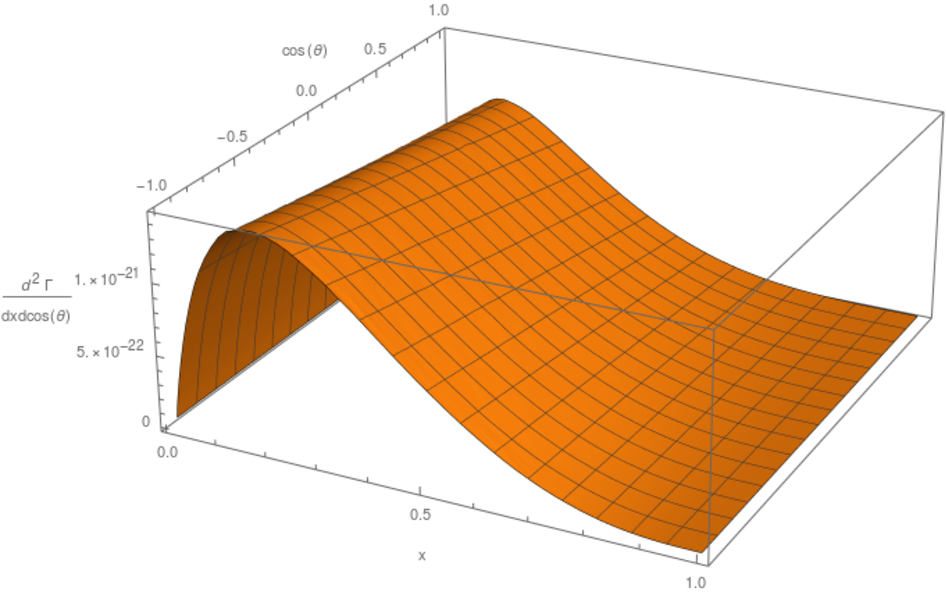
\includegraphics[width=\linewidth]{imgs/ScalarElectronPlot}
  \caption{Spectrum with $m_\phi=\SI{10}{\mega \eV}$ and coupling to the electron}
  \label{fg:ScaElSpectrum}
\end{subfigure}%
\begin{subfigure}{.45\textwidth}
  \centering
  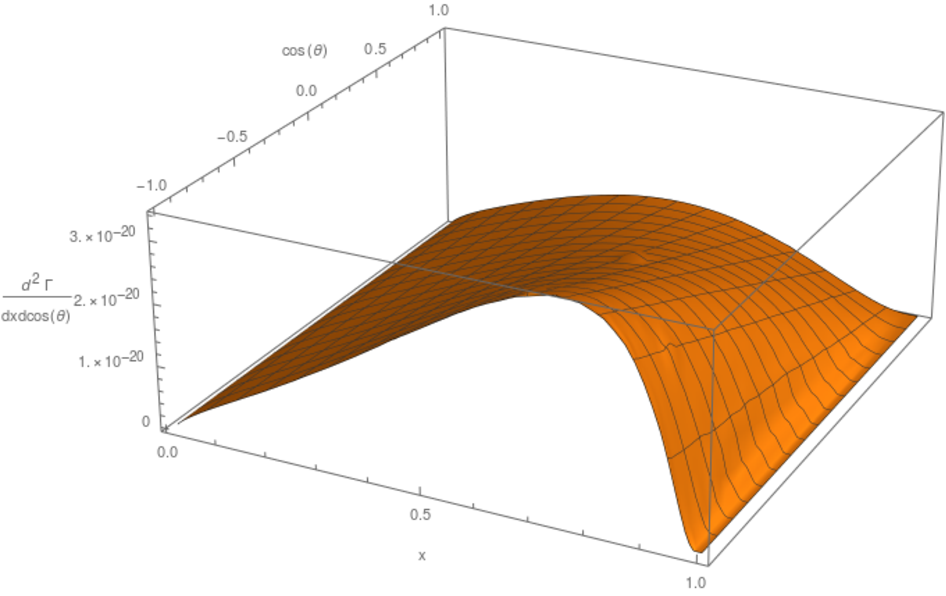
\includegraphics[width=\linewidth]{imgs/VectorLeptonPlot}
  \caption{Spectrum with $m_{A'}=\SI{10}{\mega \eV}$ and $L_e-L_\mu$ couplings}
  \label{fg:VecLepSpectrum}
\end{subfigure}
\caption{Example spectra}
\label{fg:exampleSpectra}
\end{figure}
\section{Validity checks}
The resulting spectrum need to be checked for validity to determine, whether the number of nodes is enough to resolve the structure of the integrand. First, for each scenario the remaining two sums are carried out to get the total decay width. This is then compared to the decay width as calculated by the tool \textsc{Calc-HEP} that is configured such that the estimated error is less than one part per thousand. Then both widths are compared. For $(N(E_1),N(E_1),N(\theta_1),N(\theta_2),N(\theta_3),N(\phi_1),N(\phi_2)=(60,60,60,25,25,25,25)$ both width easily agree. 
\section{Michel parameter extraction}
The spectra have been calculated with all BSM coupling constants set to unity. Now the known standard model decay spectrum from equation \ref{eq:Diffrate} is added to the BSM-spectrum that has been scaled by a factor $g^2$. This is then subject to a similar fitting routine as the experimentalists used to extract the values for $\rho$, $\delta$ and $\xi$. The overall scale factor in the experimental setup would be fixed by the total number of included events. Here the combination of both decay widths replaces this.
$g^2$ is then varied and the bisection method is used to find its maximum value that violates one or more of the expected values by $2\sigma$.
Then $g$ can be used as a bound on the BSM-coupling.
\section{Influence of the fiducial region}
The authors of \cite{TWIST:2011aa} had to restrict the part of the spectrum that was used to extract the Michel parameters because of the detector geometry and inefficiencies. The region used is shown in figure \ref{fg:FiducialRegion}. If the BSM-spectrum was concentrated outside the fiducial region, its influence would be greatly underestimated. To get comparable results, either the same region has to be used or the influence has to be tested as to make sure it can be neglected. 
\begin{figure}[ht]
  \centering
    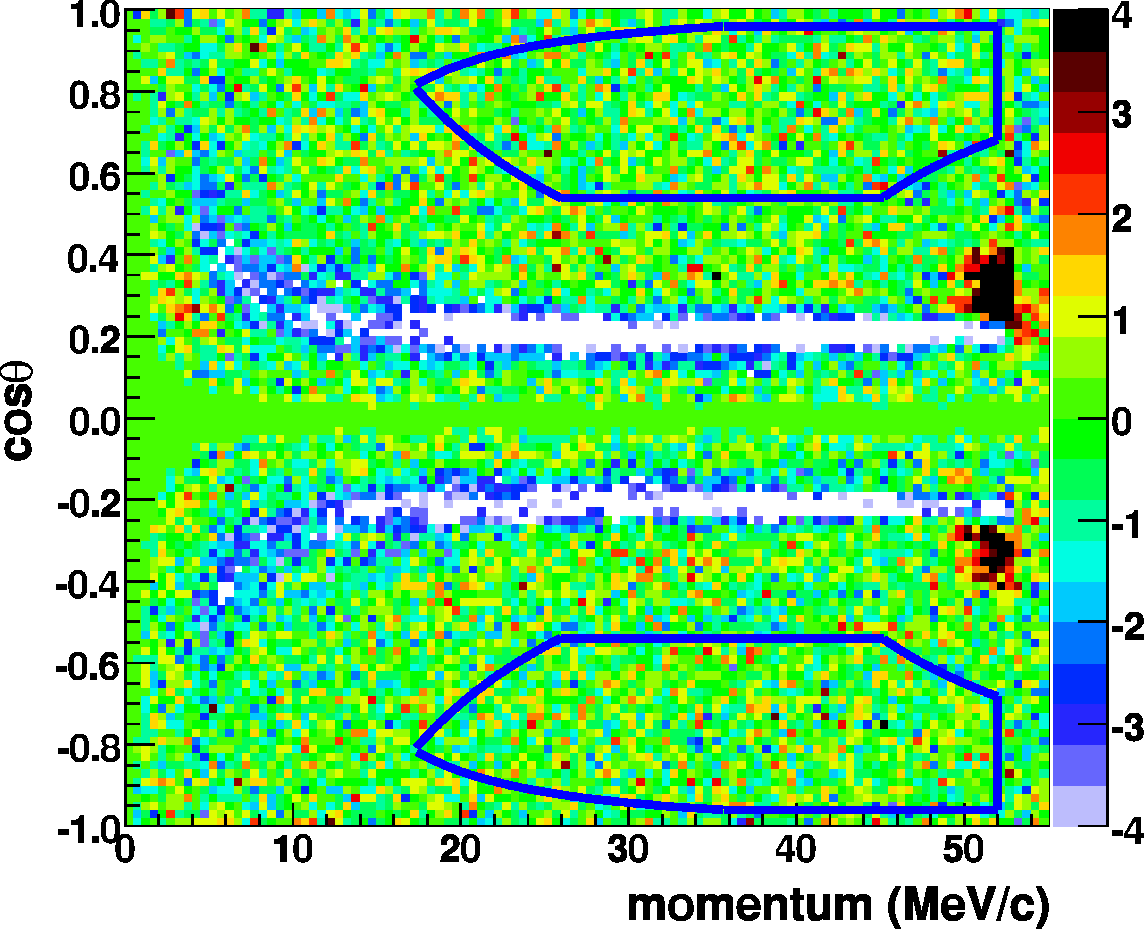
\includegraphics[width=0.6\textwidth]{imgs/fiducial}
    \caption{Fiducial region (blue) used by \cite{TWIST:2011aa}}
    \label{fg:FiducialRegion}
\end{figure}
Figure \ref{fg:MassDependence} shows the form of the spectra depending on the mediator mass. Clearly the bulk of the spectrum is included in the fiducial region, so that the experimental setup isn't accidentally blind to these processes. Only the heaviest mediators with masses $\geq \SI{50}{\mega \eV}$ avoids the active region. But the corresponding bounds are weak anyway because of the small width and are not competitive with existing bounds. 
The restriction to these regions worsens the bound only by a factor of order one where for almost all mass choices the bounds get weaker by a factor between two and four.
\begin{figure}[H]
	\centering
	\begin{subfigure}[b]{0.45\textwidth}
    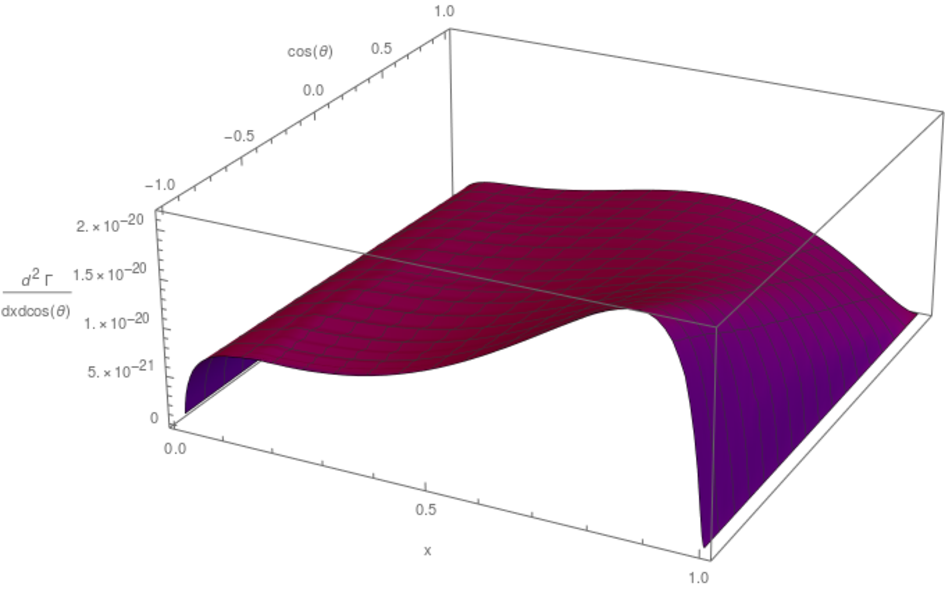
\includegraphics[width=\textwidth]{imgs/S0-001}
    \caption{$m_\phi = 1$MeV}
    \end{subfigure}
    ~
    \begin{subfigure}[b]{0.45\textwidth}
    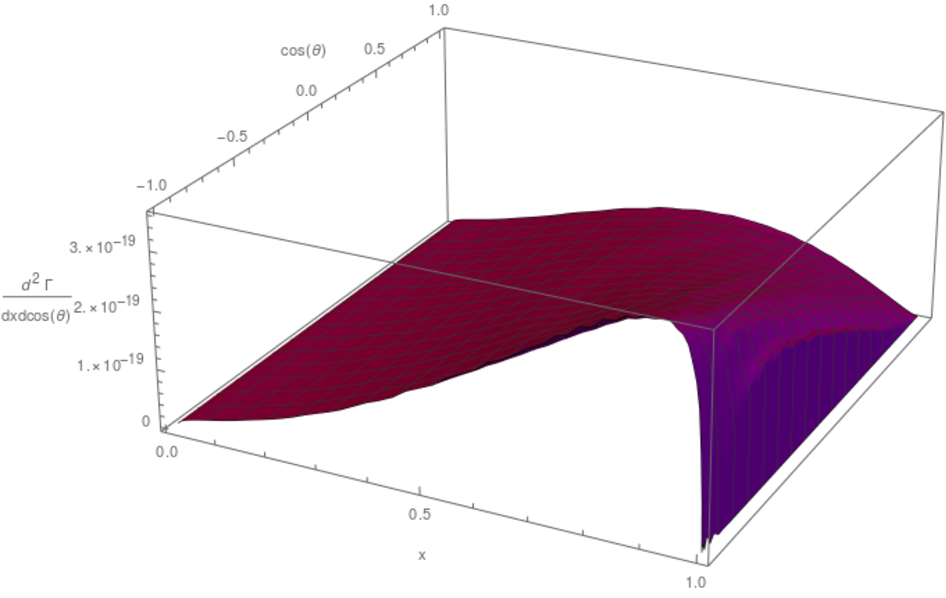
\includegraphics[width=\textwidth]{imgs/V0-001}
    \caption{$m_{A'} = 1$MeV}
    \end{subfigure}
    
    \begin{subfigure}[b]{0.45\textwidth}
    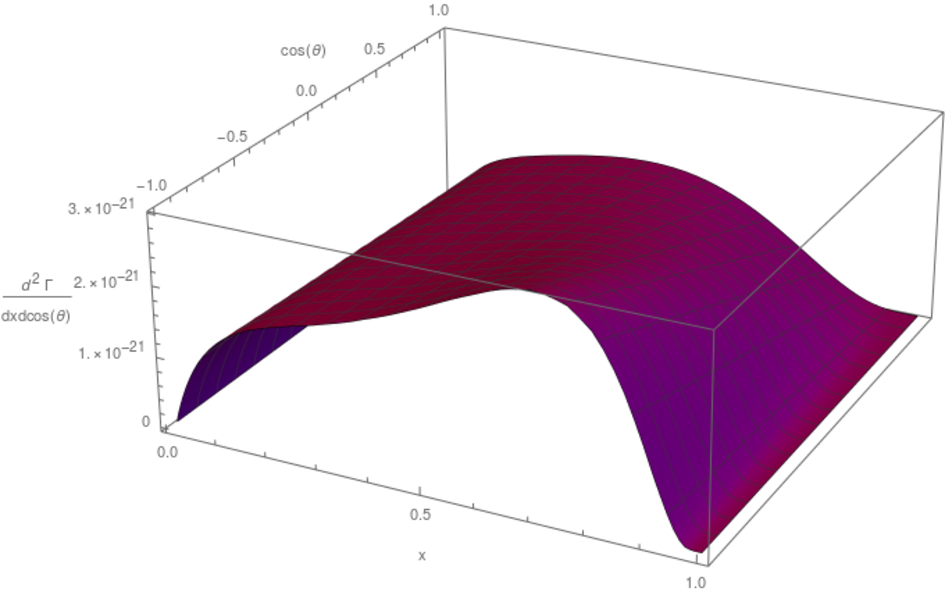
\includegraphics[width=\textwidth]{imgs/S0-01}
    \caption{$m_\phi = 10$MeV}
    \end{subfigure}
    ~
    \begin{subfigure}[b]{0.45\textwidth}
    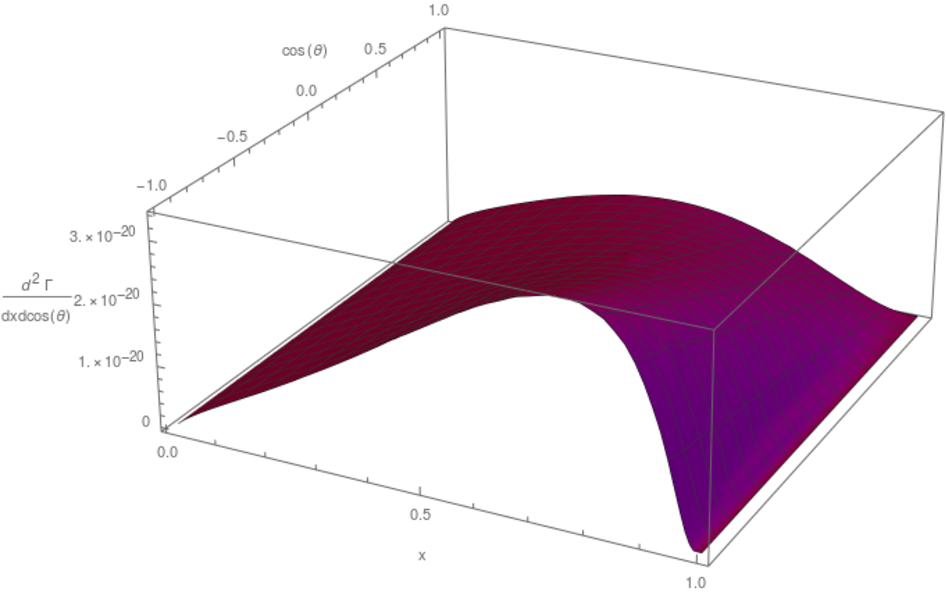
\includegraphics[width=\textwidth]{imgs/V0-01}
    \caption{$m_{A'} = 10$MeV}
    \end{subfigure}
    
    \begin{subfigure}[b]{0.45\textwidth}
    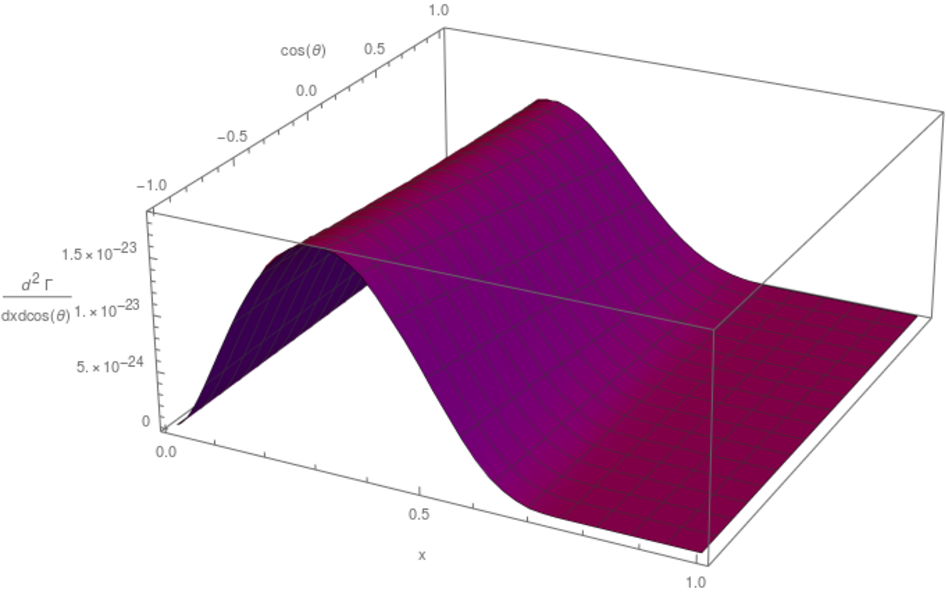
\includegraphics[width=\textwidth]{imgs/S0-05}
    \caption{$m_\phi = 50$MeV}
    \end{subfigure}
    ~
    \begin{subfigure}[b]{0.45\textwidth}
    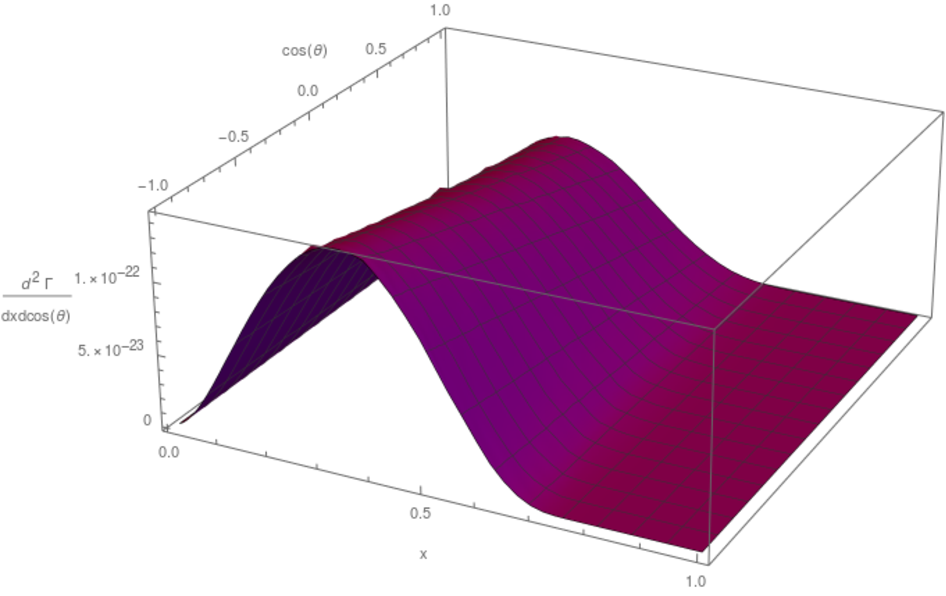
\includegraphics[width=\textwidth]{imgs/V0-05}
    \caption{$m_{A'} = 50$MeV}
    \end{subfigure}
    \caption{Scalar (left) and vector (right) mass dependence of the spectra}
    \label{fg:MassDependence}
\end{figure}
\newpage
\section{Results}
Here the resulting bounds on the couplings will be presented and compared to existing constraints. Because the existing literature doesn't use consistently either 90 \% or 95\% C.L. exclusions, both are shown in each graph. 
\subsection{Scalar Mediator}

\begin{figure}[!ht]
  \centering
    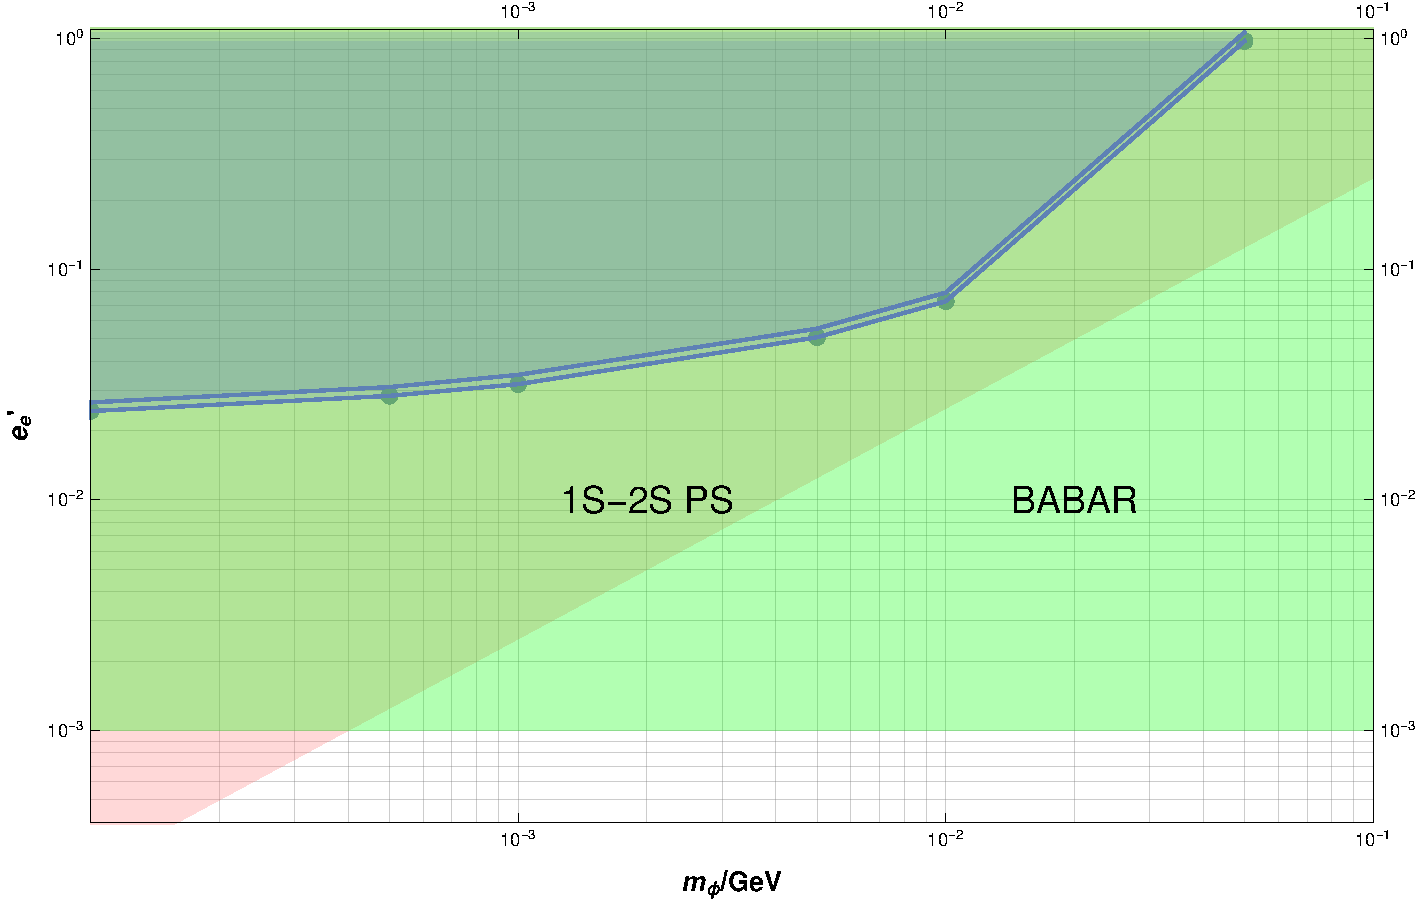
\includegraphics[width=0.8\textwidth]{imgs/MuBoundOnScalarElectron.pdf}
    \caption{90\% and 95\% C.L. bounds on the scalar-electron coupling (blue) with existing bounds from 1S-2S transitions in positronium (brown 95\% C.L.) and missing energy searches by BABAR (green, 95\%C.L.) \cite{Essig:2013vha}}
    \label{fg:MuBoundScEl}
\end{figure}
Shown in figure \ref{fg:MuBoundScEl} are the bound on the coupling between the electron and a scalar mediator. 

\begin{figure}[!ht]
  \centering
    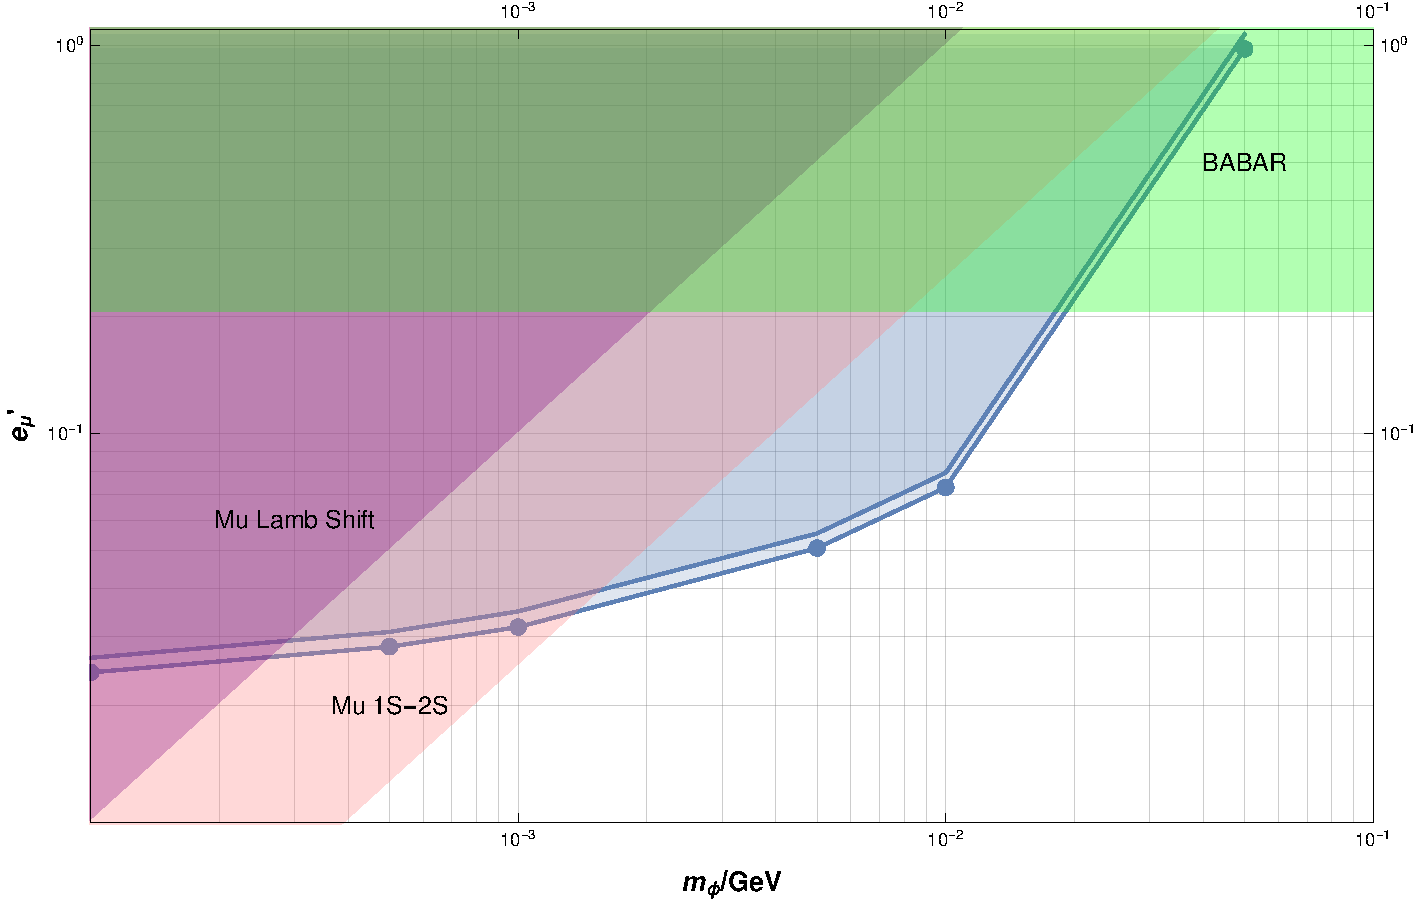
\includegraphics[width=0.8\textwidth]{imgs/MuBoundOnScalarMuon.pdf}
    \caption{90\% and 95\% C.L. bounds on the scalar-muon coupling (blue) and existing bounds for a hierarchical coupling to both lepton families from the Lamb-shift and 1S-2S transition in muonium (purple and red respectively, 95\% C.L.)}
    \label{fg:MuBoundScMu}
\end{figure}
Figure \ref{fg:MuBoundScMu} shows the bounds for the coupling between the muon alone and the scalar mediator that are only slightly stronger than the electron case. This model specifically has not been constrained without further assumptions. Here it is compared to a somewhat better motivated model with mass-hierarchical couplings $e_e'/e_\mu'=m_e/m_\mu$. With this assumption bounds on the product of the couplings $e_e'\times e_\mu'$ from lamb shifts and 1S-2S transitions in muonium can be converted to bounds on the scalar-muon coupling $e_\mu' = \sqrt{e_e'\times e_\mu'\cdot m_\mu/m_e}$. These again have already ruled out most of the parameter space that can be excluded with the muon spectrum. 
\subsection{Vector Mediator}

\begin{figure}[H]
  \centering
    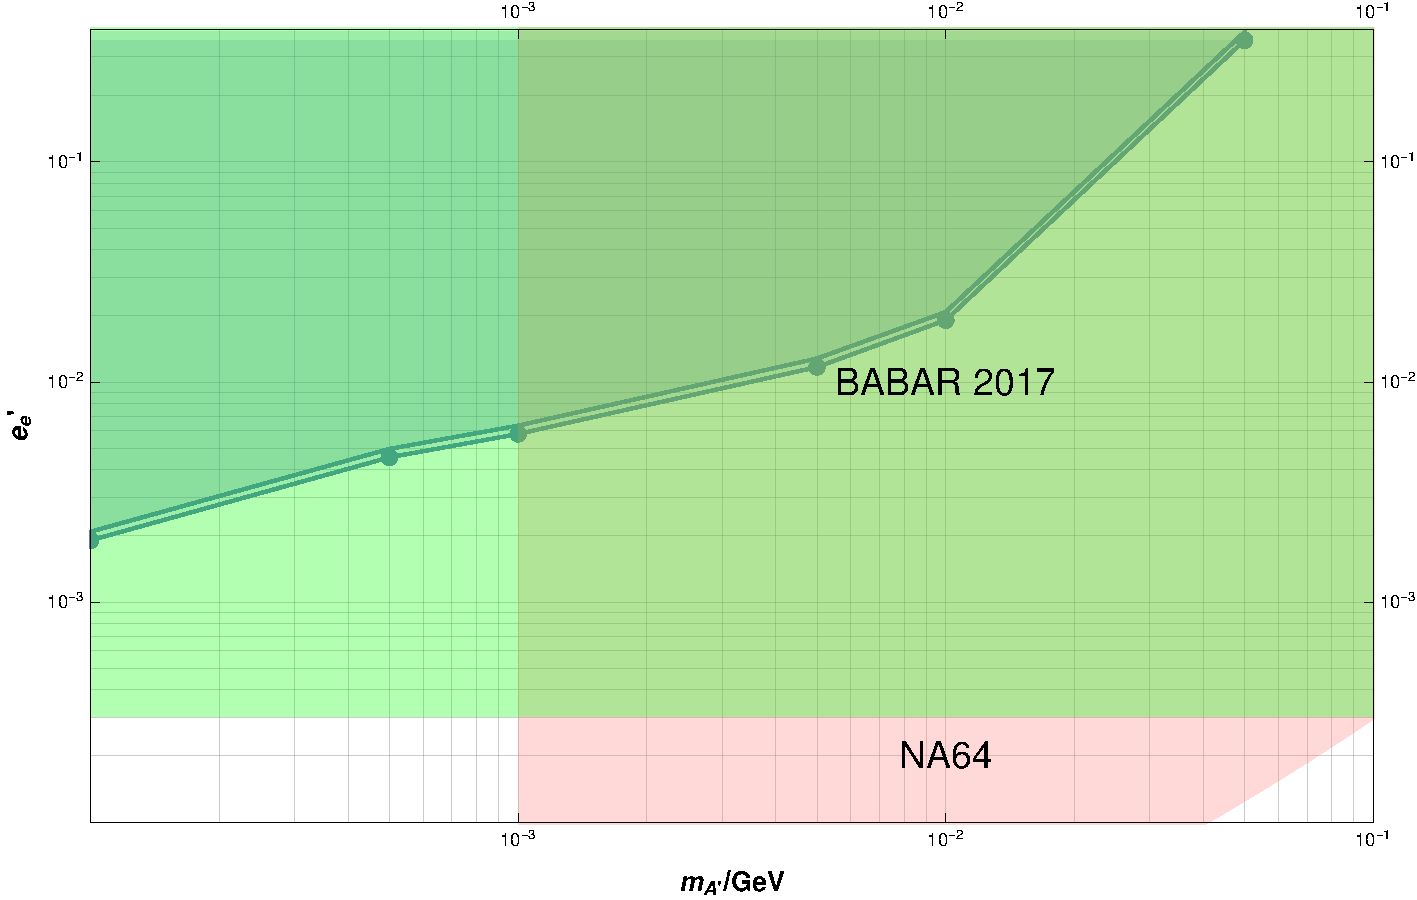
\includegraphics[width=0.8\textwidth]{imgs/MuBoundOnVectorElectron.pdf}
    \caption{90\% and 95\% C.L. bounds on the vector-electron coupling (blue) with existing bounds by NA64 (red 90\% C.L.) and BABAR (green 90\% C.L.)}
    \label{fg:MuBoundVeEl}
\end{figure}
Figure \ref{fg:MuBoundVeEl} shows the bounds on the coupling constants between the muon and a vector mediator alone. The parameter space that could be ruled out with the muon decay has already been constrained by missing energy searches by BABAR and NA64 although the NA64 bounds are only applicable for $m_{A'}>\SI{1}{\mega \eV}$.

\begin{figure}[H]
  \centering
    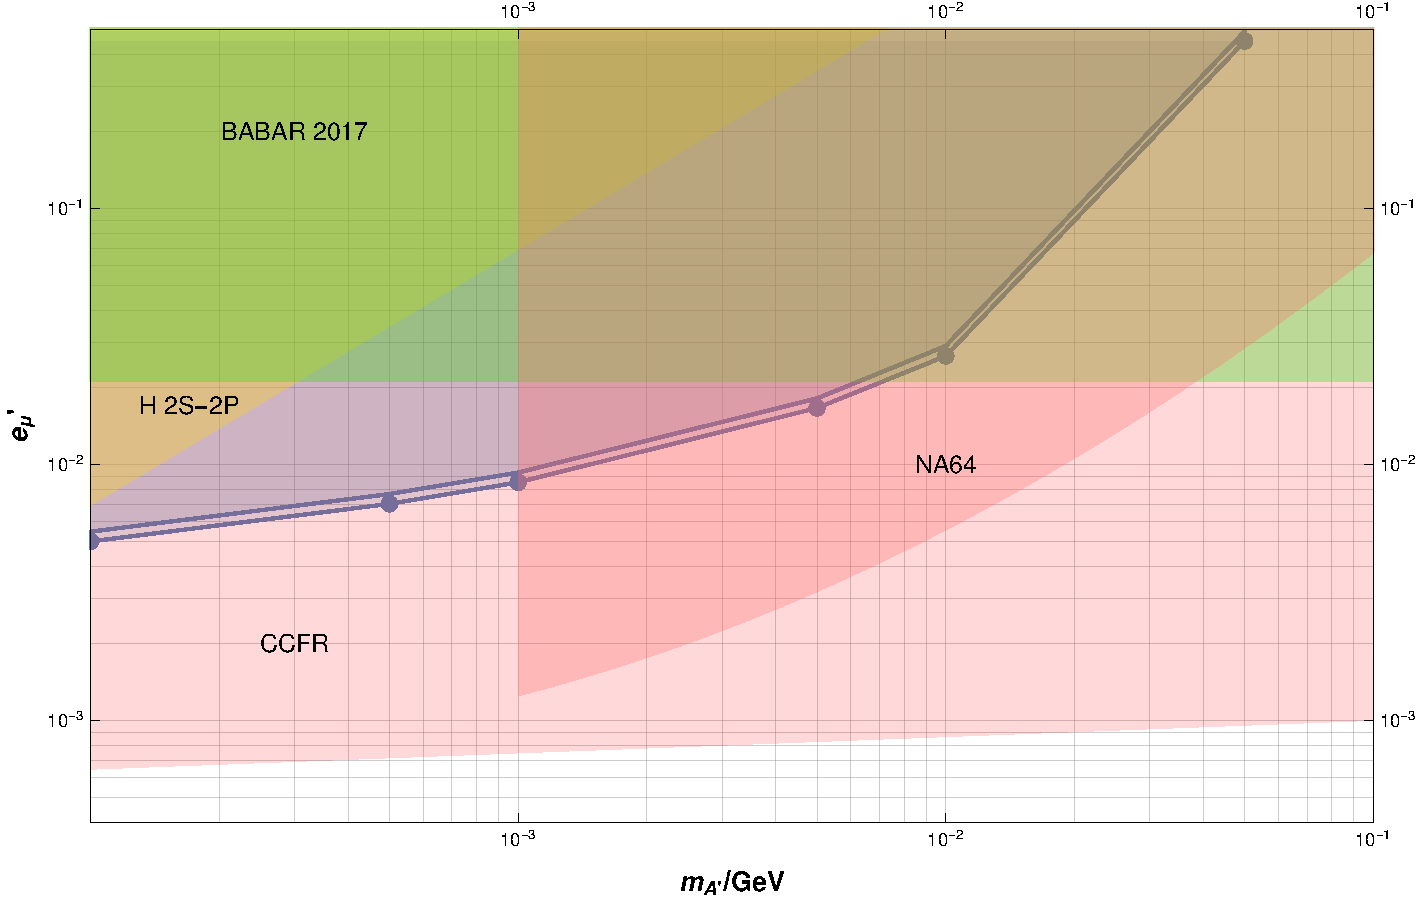
\includegraphics[width=0.8\textwidth]{imgs/MuBoundOnVectorMuon.pdf}
    \caption{90\% and 95\% C.L. bounds on the vector-muon coupling (blue) with existing bounds for the specific $L_{\mu-\tau}$ model by NA64 (red 90\% C.L.) and BABAR (green 90\% C.L.) and hydrogen 2S-2P transition (yellow 95\% C.L.) and neutrino trident production from CCFR (light pink 95\% C.L.)}
    \label{fg:MuBoundVeMu}
\end{figure}
Figure \ref{fg:MuBoundVeMu} shows bounds from the muon decay with only a direct coupling between the muon and the vector mediator. Again since the model with direct coupling only to one lepton family contains anomalies and isn't well motivated there are few existing bounds besides from neutrino trident production shown in the graph. Out of the anomaly free models with gauged $L_{B-L},L_{e-\mu}$ or $L_{\mu-\tau}$ the latter will result in the weakest existing bounds. The resulting expression for the 1-loop kinetic mixing can then be used to translate the existing bounds on the kinetic mixing parameter $\epsilon$ from the NA64 and BABAR experiments to bounds on $e_\mu'$ shown. Additionally to these bounds from hydrogen 2S-2P transitions are used. 
\begin{figure}[H]
  \centering
    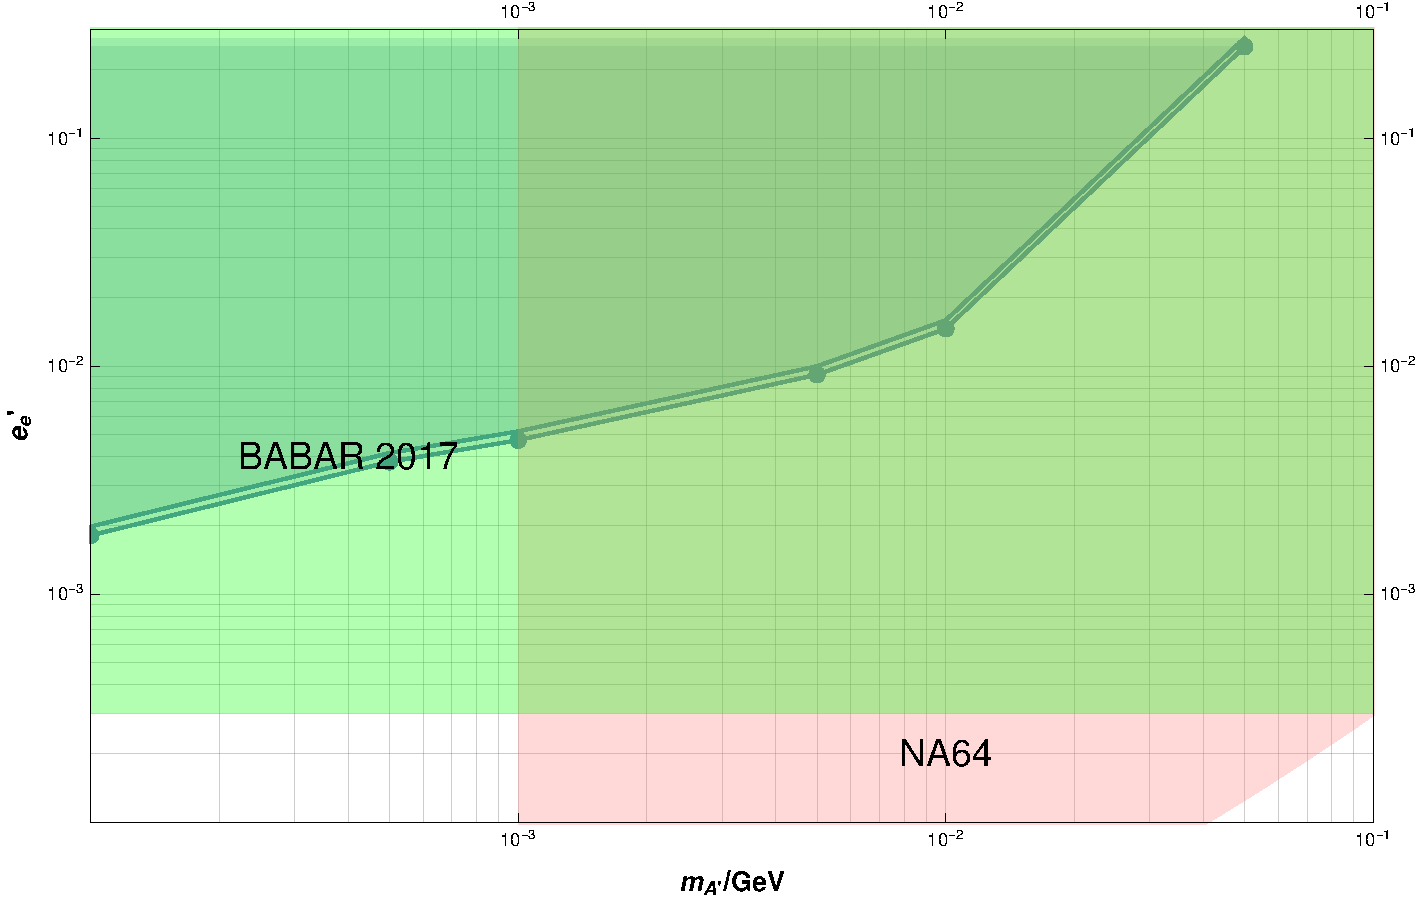
\includegraphics[width=0.8\textwidth]{imgs/MuBoundOnVectorLepton.pdf}
    \caption{90\% and 95\% C.L. bounds on the vector-lepton ($e_e'=-e_\mu'$) coupling (blue) with existing bounds by NA64 (red 90\% C.L.) and BABAR (green 90\% C.L.)}
    \label{fg:MuBoundVeEM}
\end{figure}

Lastly figure \ref{fg:MuBoundVeEM} shows bounds for the model with gauged $L_{e-\mu}$. Here again the bounds from BABAR and NA64 directly apply without further specifications.

\section{Discussion}
The bounds on the electron-scalar coupling obtained here are already ruled out by the BABAR data and the 1S-2S transition in positronium independently. An improvement of the experimental values of the Michel parameters of about three orders is needed to compete with the BABAR result. So this model will not be further constrained using the muon decay in the near future. 

Similar bounds for the muon specific scalar interaction has not been considered in the literature. These results can be compared to to the mass hierarchical coupling between the scalar and the standard model leptons. This way the muon results are related to the electron coupling bounds, though considerably weaker. Additionally results from muonium spectrography become applicable. Compared to these constraints, the ones from the muon decay exclude an additional section of parameter space for mediator masses between 2 and \SI{20}{\mega \eV}.

The constraints on the coupling between the vector mediator and the electron are again much weaker than those obtained by BABAR. Below a mediator mass of \SI{1}{\mega \eV} the uncertainties of the Michel parameters have to be improves only by two orders. NA64 becomes applicable above \SI{1}{\mega \eV} so even a great precision improvement in the muon decay will not become competitive here.

The coupling between the muon and the vector mediator will again need more care. Here the gauged $L_{\mu-\tau}$ model is chosen for comparison. Since this lacks a tree-level coupling to the electron it avoids the generally strong constraints but can nevertheless be implemented anomaly free. Here the kinetic mixing
\begin{equation}
\epsilon = \frac{ee'_\mu}{12\pi^2}\ln\left(\frac{m_\tau^2}{m_\mu^2}\right)
\end{equation}
with $e'_\mu=-e'_\tau$ is used to convert bounds on $\epsilon$ or even to the electron alone to constraints on $e'_\mu$. The results from BABAR alone are in this case weaker than the muon decay results. With the inclusion of the NA64 results no new constraints could be derived for mediator masses above \SI{1}{\mega\eV}. Below the neutrino trident production results from CCFR are used for comparison. Since these apply directly at tree-level without a loop, it results in stronger constraints that already ruled out the results from the muon spectrum. Also shown is the bound from 2S-2P transitions in hydrogen. 

The last considered model with gauged $L_{e-\mu}$ couples to all involved particles. But since it has a tree level coupling to the electron, the BABAR results apply directly and the bounds are not competitive. Here only the bounds on masses below \SI{1}{\mega \eV} will become competitive if the uncertainties are improved by two orders of magnitude. Otherwise an improvement by at least three orders would be needed. This should be well out of reach of experiments in the near future.

A widening of the fiducial region by means of detector improvements will not lead to competitive bounds, even for a perfect detector that is capable to reliably observe the whole spectrum. 
\newpage
\chapter{SM-Pion Decay}
\label{ch:SM-PionDecay}
The decay of a charged pion can be described in the framework of chiral perturbation theory.
The applicable terms of the Effective Lagrangian regarding the leptonic charged pion decay are \cite{Scherer:2002tk} 
\begin{align*}
\mathcal{L} \supset &-\frac{g}{2\sqrt{2}}\sum_{l=e,\mu}\left[W_\mu^+\bar{\nu}_l \gamma^\mu(1-\gamma_5)l +W_\mu^-\bar{l}\gamma^\mu(1-\gamma_5)\nu_l\right]\\
&-g\frac{F_0 V_{ud}}{2}\left[ W^+_\nu\partial^\nu\pi^-+W^-_\nu\partial^\nu\pi^+\right]
\end{align*}
where $g$ is the SU(2) gauge coupling, $V_{ud}$ the Cabibbo-Kobayashi-Maskawa matrix element for the up- and down-quark and $F_0$ the pion-decay constant.
Now consider the decay to the lepton $l$ and its neutrino $\nu_l$ with the following Feynman diagram:
\begin{figure}[!h]
\centering
\begin{tikzpicture}
\begin{feynman}
\vertex (a) {\(\pi^{+}\)};
\vertex [right=of a] (b);
\vertex [right=of b] (c);
\vertex [above right=of c] (f1){\(\nu_l\)};
\vertex [below right=of c] (f2){\(l^+\)};
\diagram* {
(a) -- [scalar] (b) -- [boson, edge label'=\(W^{+}\)] (c),
(c) -- [fermion] (f1),
(c) -- [anti fermion] (f2)
};
\end{feynman}
\end{tikzpicture}
\end{figure}
Using the Fermi constant
\begin{equation}
G_f= \frac{g^2}{4\sqrt{2}M_w^2}
\end{equation}
it leads to the associated decay width
\begin{equation}
\label{eq:Pion_Wdth}
\Gamma = \frac{G_f^2 |V_{ud}|^2}{4\pi}F_0^2 m_\pi m_l^2\left(1-\frac{m_l^2}{m_\pi^2}\right)^2
\end{equation}
where the factor $\sim m_l^2$ points to the helicity suppression of the charged pion decays to leptons. Intuitively this is to to the pions spin being 0, so that both final states fermions have to have opposite spin alignment. Since its a two body decay, the momentum also points in opposite directions so that both particles have the same helicity. Now from the weak interaction only couples to the left chiral neutrino so since its massless its helicity is also left-handed. So the positron is also left handed which suppresses the decay since it was produced as a left chiral anti particle (for massless particles, left chiral antiparticles have right helicity) and need a mass insertion to be allowed.
After using the lifetime of the pion of $2.6\cdot 10^{-8}s$ to fix the value of $F_0$ equation \ref{eq:Pion_Wdth} leads to the branching ratio to first order
\begin{equation}
\frac{\Gamma(e^+ \nu_e)}{\Gamma(\mu^+ \nu_\mu)}=\frac{m_e^2}{m_\mu^2}\frac{\left(1-\frac{m_e^2}{m_\pi^2}\right)^2}{\left(1-\frac{m_\mu^2}{m_\pi^2}\right)^2} \approx 1.28\cdot 10^{-4}
\end{equation}.
This observable can be measured more easily by including the decays with photons.
Work done by Cirigliano and Rosell \cite{PhysRevLett.99.231801} calculates its value to two loop order in chiral perturbation theory as
\begin{equation}
R^\pi_{e/\mu} \equiv \frac{\Gamma(e^+ \nu_e(\gamma))}{\Gamma(\mu^+ \nu_\mu(\gamma))}=(1.2352	\pm0.0001)\cdot 10^{-4}
\end{equation}
which is in good agreement with the experimental value of
\begin{equation}
R^\pi_{e/\mu} =(1.2344\pm 0.0023\text{(stat.)} \pm 0.0019\text{(syst.)})\cdot 10^{-4}
\end{equation}
found by Aguilar-Arevalo \cite{PhysRevLett.115.071801}.
\newpage
\chapter{Bounds from \texorpdfstring{$\pi^+$}{pion} decay spectrum}
\label{ch:BoundsPI}
As was seen in the previous section, pions decay almost exclusively in a muon and the corresponding neutrino. The clean background and theoretically well understood decay mode establish it as a useful scenario to investigate BSM models that influence the decay. For this work the most important feature are the two final state leptons. 
The simplicity of the production and identification of pions in collider experiments provide a rich experimental data source. 
One data set that can be used to constrain leptophilic mediator models is found in \emph{Improved Search for Heavy Neutrinos in the Decay $\pi\rightarrow e\nu$} \cite{Aguilar-Arevalo:2017vlf} by the PIENU Collaboration. 
The aim of this collaboration was to measure the  branching ration $R_{e/\mu}^\pi$ and thus test lepton universality more precise than ever before. 
The experiment used TRIUMFs M13 beam of pions that were creates by a proton beam hitting a Beryllium target. The fragments were then selected and collimated to form the pion beam consisting of 84\% $\pi^+$, 14\%$\mu^+$ and 2\%$e^+$. 
Pions were then distinguished from the other constituents by their energy loss in scintillators and subsequently stopped in the detector. These then decayed at rest. 
The resulting positron energy spectrum contains besides the pure $\pi^+\rightarrow e^+\nu_e$ decays also positrons from the decay chain $\pi^+\rightarrow \mu^++\nu_\mu \rightarrow e^+ \nu_e +\nu_\mu$ that are distinguished by fitting to Monte Carlo simulations or their timing and direction. 
The total spectrum and its constituents are shown in figure \ref{fg:PiENuSpectrum}.
\begin{figure}[H]
  \centering
    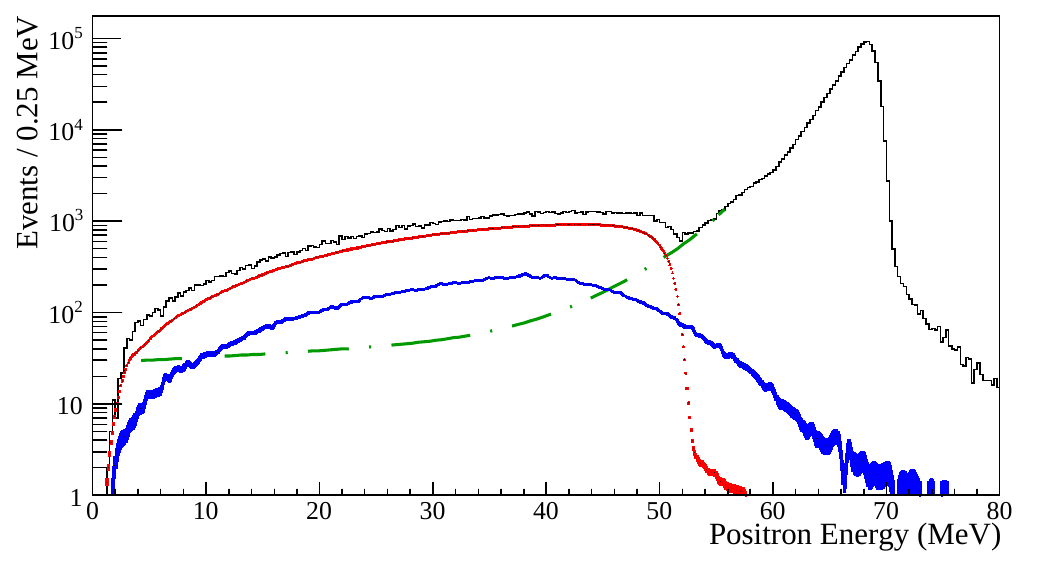
\includegraphics[width=0.8\textwidth]{imgs/graph}
    \caption{Backgound suppressed positron spectrum (black), with components from muon decays in flight (blue), $\pi^+\rightarrow e^+\nu_e$ (green) and $\pi^+\rightarrow \mu^++\nu_\mu \rightarrow e^+ \nu_e +\nu_\mu$ (red)
    taken from \cite{Aguilar-Arevalo:2017vlf}}
    \label{fg:PiENuSpectrum}
\end{figure}
The difference between the data and the fit can then be used to look for signs of new physics. This was then used to look for extra peaks is the spectrum that would indicate heavy neutrinos. The absence of any additional structure was used to constrain the neutrino mixing matrix elements in the mass region $60-135$MeV at 90\% C.L.

The same data set can conveniently be used to search for other sources of new physics. Most important in this work the diagram shown in figure \ref{fg:PiENuBSMGraphsScalar} can be used to extract constraints on the electron-scalar mediator coupling,
\begin{figure}[H]
\centering
\scalebox{1}{%
\begin{tikzpicture}
\begin{feynman}
\vertex (a) {\(\pi^{+}\)};
\vertex [right=of a] (b);
\vertex [right=of b] (c);
\vertex [above right=of c] (f1){\(\nu_e\)};
\vertex [below right=of c] (d);
\vertex [above right=of d] (f2){\(\phi\)};
\vertex [below right=of d] (f3){\(e^+\)};
\diagram* {
(a) -- [scalar] (b) -- [boson, edge label'=\(W^{+}\)] (c),
(c) -- [fermion] (f1),
(c) -- [anti fermion] (d),
(d) -- [anti fermion] (f3),
(d) -- [scalar] (f2)
};
\end{feynman}
\end{tikzpicture}
}

\caption{Pion-decay contribution with a scalar mediator}
\label{fg:PiENuBSMGraphsScalar}
\end{figure}
while the diagrams shown in figure \ref{fg:PiENuBSMGraphsVector} can be used to constrain the dark photon model where the vector couples to the electron. 
\begin{figure}[h]
\centering
\begin{subfigure}{.5\textwidth}
\centering
  \begin{tikzpicture}
\begin{feynman}
\vertex (a) {\(\pi^{+}\)};
\vertex [right=of a] (b);
\vertex [right=of b] (c);
\vertex [above right=of c] (f1){\(\nu_e\)};
\vertex [below right=of c] (d);
\vertex [above right=of d] (f2){\(A'\)};
\vertex [below right=of d] (f3){\(e^+\)};
\diagram* {
(a) -- [scalar] (b) -- [boson, edge label'=\(W^{+}\)] (c),
(c) -- [fermion] (f1),
(c) -- [anti fermion] (d),
(d) -- [anti fermion] (f3),
(d) -- [boson] (f2)
};
\end{feynman}
\end{tikzpicture}
\end{subfigure}%
\begin{subfigure}{.5\textwidth}
\centering
\begin{tikzpicture}
\begin{feynman}
\vertex (a) {\(\pi^{+}\)};
\vertex [right=of a] (b);
\vertex [right=of b] (c);
\vertex [above right=of c] (d);
\vertex [above right=of d] (f1){\(\nu_e\)};
\vertex [below right=of d] (f2){\(A'\)};
\vertex [below right=of c] (f3){\(e^+\)};
\diagram* {
(a) -- [scalar] (b) -- [boson, edge label'=\(W^{+}\)] (c),
(c) -- [fermion] (d)--[fermion](f1),
(c) -- [anti fermion] (f3),
(d) -- [boson] (f2)
};
\end{feynman}
\end{tikzpicture}

\end{subfigure}
\caption{Pion-decay contribution with a spin 1 mediator}
\label{fg:PiENuBSMGraphsVector}
\end{figure}
To this end, seven benchmark masses $1\cdot10^{-4}$GeV, $5\cdot10^{-4}$GeV, $1\cdot10^{-3}$GeV, $5\cdot10^{-3}$GeV, $1\cdot10^{-2}$GeV, $5\cdot10^{-3}$GeV and $1\cdot10^{-1}$GeV were chosen.
For each scenario a set of 10.000 Monte Carlo events for the new physics processes were generated. 
These were then put in a histogram that had the same binning as the dataset from the heavy neutrino search. 
\begin{equation}
\chi^2\equiv \sum^\nu_{i=1}\frac{(x_i-\mu_i)^2}{\sigma_i^2}
\end{equation}
The total number of particles in this histogram is then varied and was then subjected to a $\chi^2$ test to establish a 95\% C.L. bound on the  relative abundance of the processes in this spectrum $\alpha$. This is shown in figure \ref{fg:PionExamplePlots} for a 100MeV dark photon.
\begin{figure}[h]
  \centering
    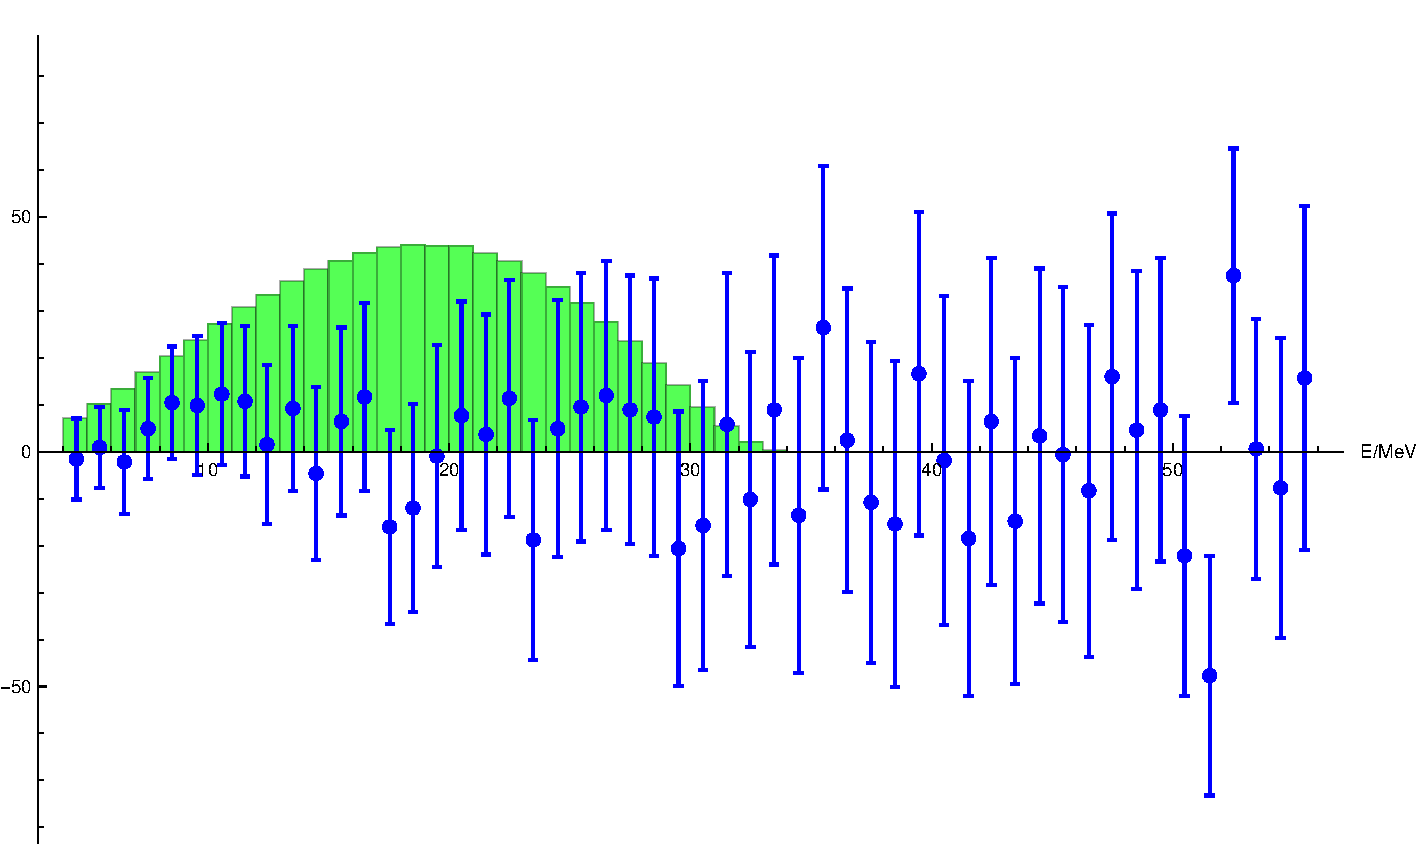
\includegraphics[width=0.6\textwidth]{imgs/PionExamplePlot}
    \caption{Datapoints from \cite{Aguilar-Arevalo:2017vlf}(blue) and positron energy spectrum for a 100MeV vector scaled such that the coupling saturates the 90\% C.L. bound} 
    \label{fg:PionExamplePlots}
\end{figure}
\begin{equation}
\alpha \gtrsim \frac{\Gamma(\pi^+\rightarrow e^+ \nu_e + \phi/A')}{\Gamma(\pi^+\rightarrow e^+ \nu_e)}
\end{equation}
This is then used to extract the coupling constants 
\begin{equation}
e_l'^2\lesssim \frac{\alpha\Gamma(\pi^+\rightarrow e^+ \nu_e)}{\Gamma(\pi^+\rightarrow e^+ \nu_e + \phi/A')|_{e_l'=1}}.
\end{equation}

\section{Results}
\begin{figure}[H]
  \centering
    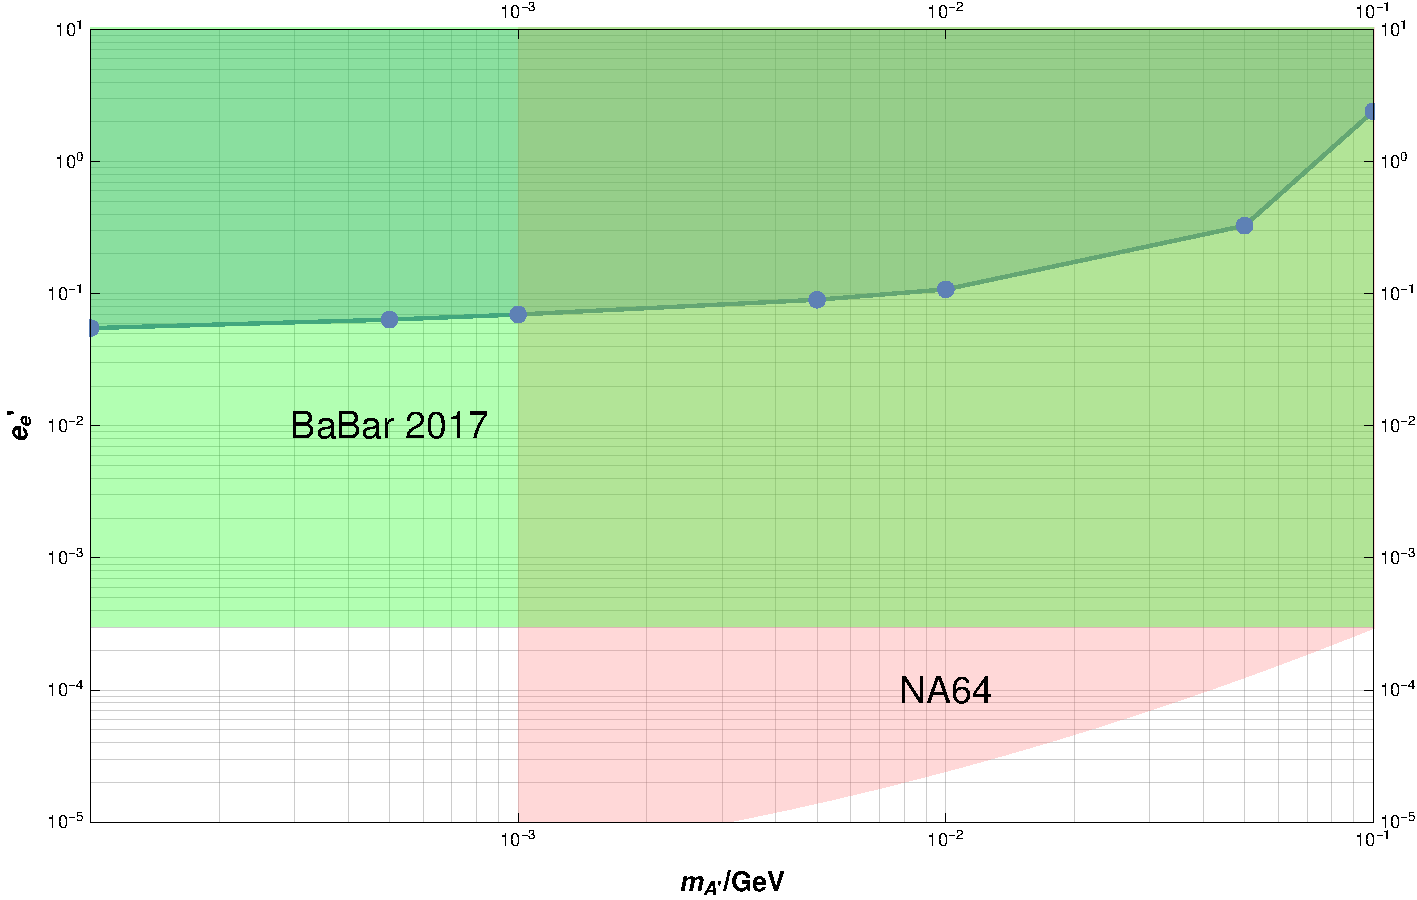
\includegraphics[width=0.8\textwidth]{imgs/PionSpectrumVector}
    \caption{95\% C.L. bounds on the vector couplings to the electron (blue)}
    \label{fg:PiSpectrumVectorBounds}
\end{figure}

\begin{figure}[H]
  \centering
    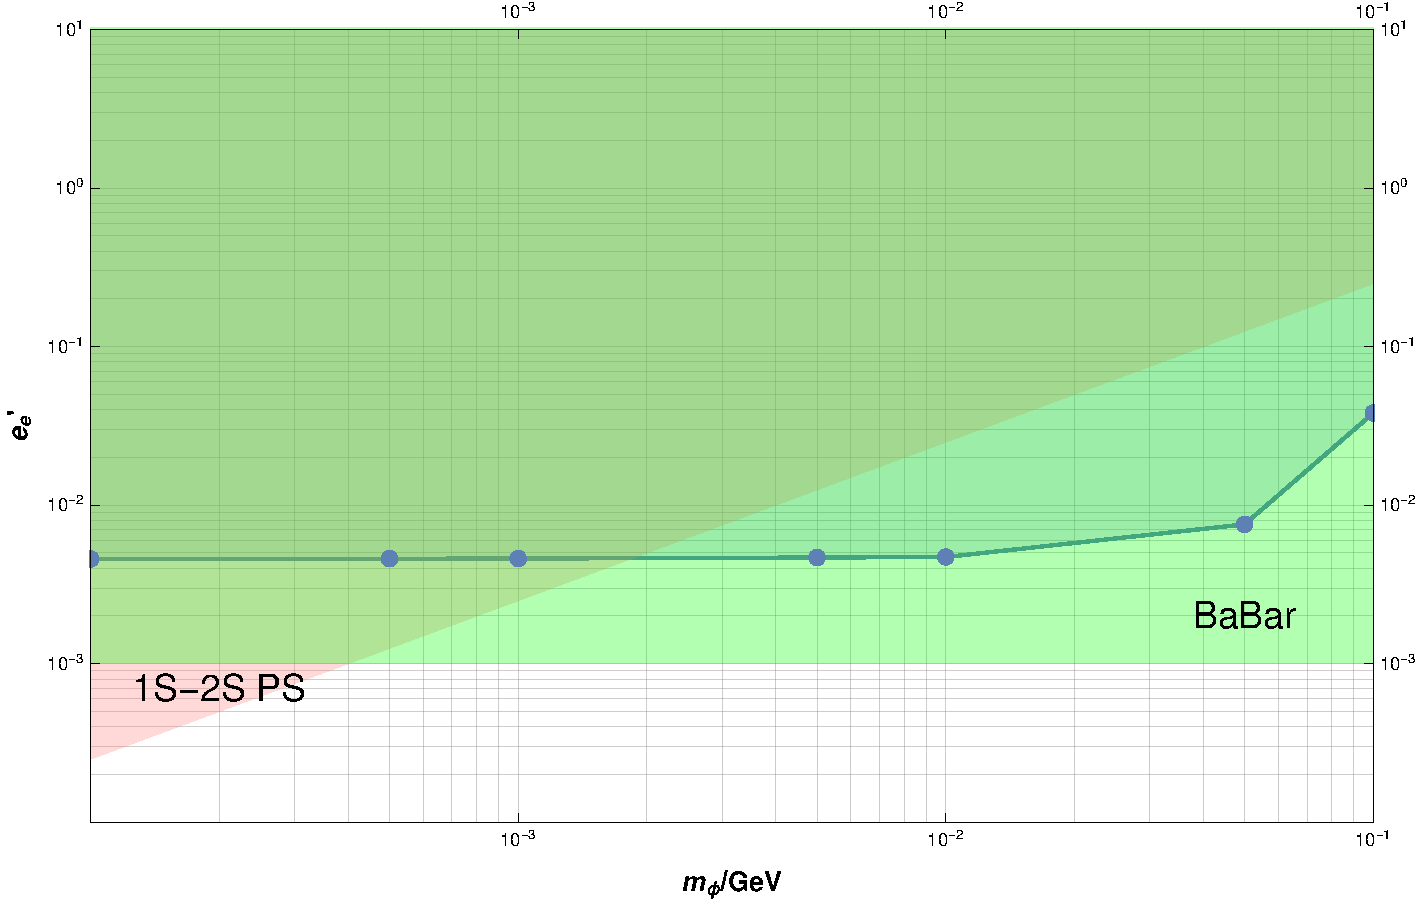
\includegraphics[width=0.8\textwidth]{imgs/PionSpectrumScalar}
    \caption{95\% C.L. bounds on the scalar couplings to the electron (blue) with bounds from 1S-2S transitions in positronium (red, 95\% C.L.) and BABAR (green, 95\% C.L.)}
    \label{fg:PiSpectrumScalarBounds}
\end{figure}

The extracted relative abundance $\alpha$ between the two models is of a similar order, despite the drastically different bounds on the couplings.  
\section{Discussion}
The bounds on the vector interaction with the electron is far from being competitive. Even strong experimental improvements will not lead to new bounds beyond the BABAR constraints.
On the other hand the bounds for the scalar interaction are much stronger, despite similar values of $\alpha$ compares to the vector case. The reason is that the scalar removes the chiral suppression whereas it stays in tact for the vector interaction. This leads to drastically larger decay width which in turn requires smaller coupling constants to be unobserved. Nevertheless this also doesn't lead to better bounds than the ones currently available. In this case a realistic improvement of experimental data could lead to better bounds than from BABAR for $m_\phi>\SI{300}{\kilo\eV}$.
\newpage
\chapter{Bounds from helicity suppression}
\label{ch:chiSupp}
The helicity suppression on its own can also be used to estimate bounds on the scalar coupling strength.
If the scalar coupling constant is large, this process contributes to searches of the violation of lepton universality in $\pi$ decays.
The width for the coupling only to the electron can be analytically calculated when the electron mass is neglected. The result is
\begin{align*}
\Gamma(e^+\nu_e\phi) =& \frac{e_e'^2 G_f^2 F_0^2 V_{ud}^2 m_\pi^3}{384\pi^3}\times \\ &\Bigg(
1-\left(\frac{m_\phi}{m_\pi}\right)^6+\left(\frac{m_\phi}{m_\pi}\right)^2\left(9+6\ln\left(\frac{m_\phi^2}{m_\pi^2}\right)\right)-\left(\frac{m_\phi}{m_\pi}\right)^4\left(9-6\ln\left(\frac{m_\phi^2}{m_\pi^2}\right)\right)
\Bigg)
\end{align*}
The fraction in front of the parentheses is given by $\approx e_e'^2 2.5\cdot 10^{-19}$GeV where the rest is essentially the closing phase space, which is constant 1 for $m_\phi<14$ MeV. This mode lets the pion decay to an electron (and the invisible scalar) even when the electron mass is zero.
 This additional process would then in turn change the ratio of decay widths mentioned before to
\begin{equation}
R_{e/\mu}'^\pi=\frac{\Gamma(e^+ \nu_e(\gamma))+\Gamma(e^+ \nu_e(\gamma)\phi)}{\Gamma(\mu^+ \nu_\mu(\gamma))+\Gamma(\mu^+ \nu_\mu(\gamma)\phi)}.
\end{equation}
where the decay $\pi^+\rightarrow \mu^+ \nu_\mu \phi(\gamma)$has only been included for completeness sake. It might be completely absent depending on the scalar coupling.
From these four additional contributions, only $\Gamma(e^+\nu_e\phi)$ has a sizeable effect, so the others are neglected. The bounds are optained by demanding, that the experimental value does not differ from the standard model prediction significantly. The corresponding bound is shown in figure \ref{fg:PiSpectrumScalarUniversalityBounds}.
\begin{figure}[H]
  \centering
    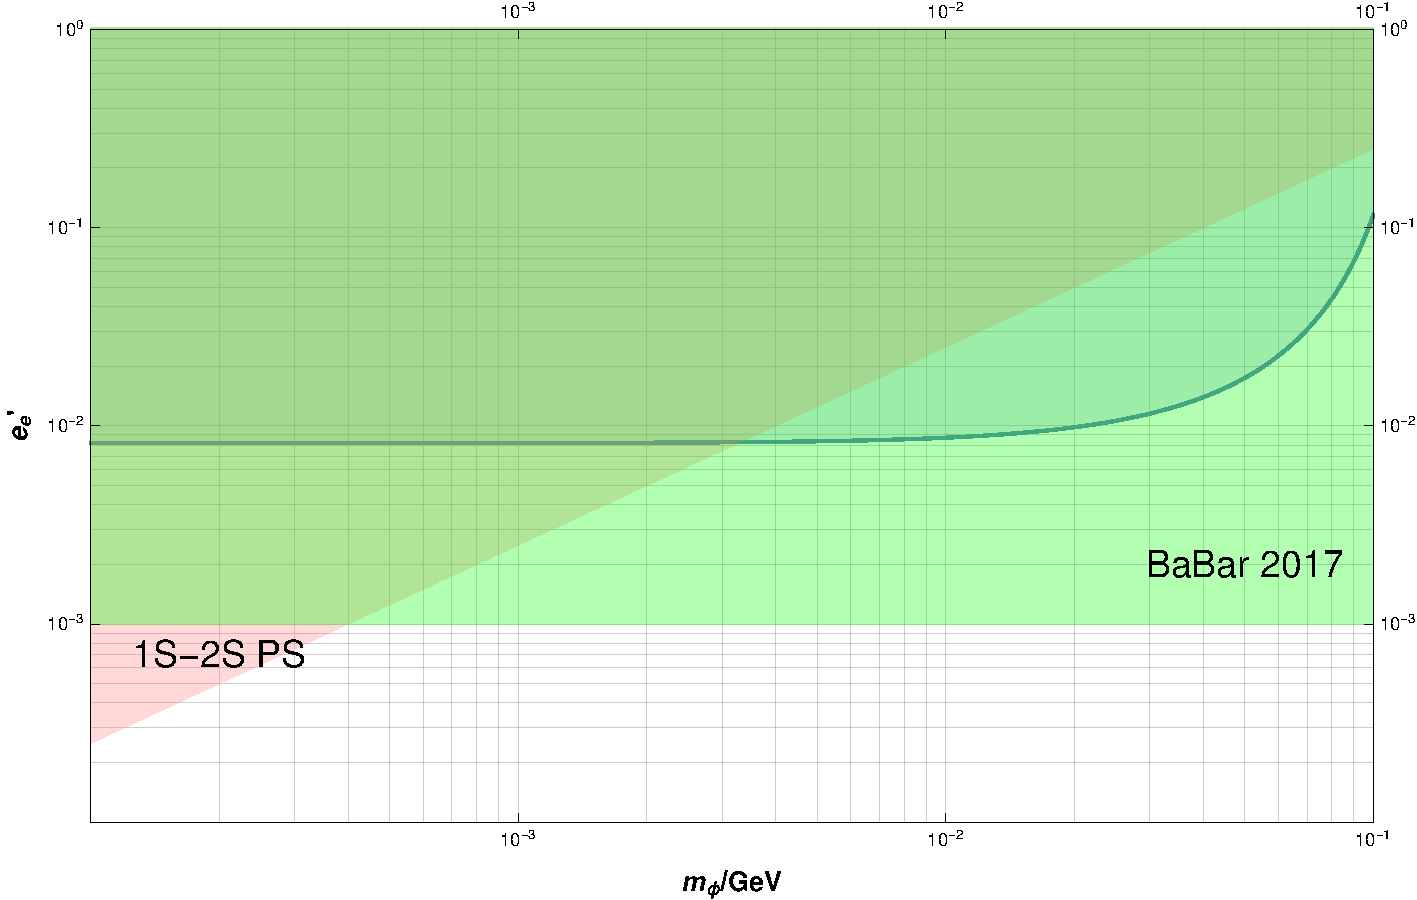
\includegraphics[width=0.8\textwidth]{imgs/LeptonUniversality}
    \caption{95\% C.L. bounds on the scalar coupling to the electron based on $R^\pi_{e/\mu}$(blue shaded) with BABAR bounds (green) and 1S-2S transitions in positronium (red)}
    \label{fg:PiSpectrumScalarUniversalityBounds}
\end{figure}
\section{Discussion}
The constraints from the removal of the chiral suppression are shown in figure \ref{fg:PiSpectrumScalarUniversalityBounds} and are again weaker than the existing bounds form BABAR. The result presented here can be generalised to $e_e'<0.008$ for $m_\phi < \SI{14}{\mega\eV}$ so even for smaller masses than shown here this bound applies. Even if the experimental precision matches the precision of the theoretical prediction, this would still not be competitive with the BABAR results.
\section{Combined Results}
\begin{figure}[ht]
  \centering
    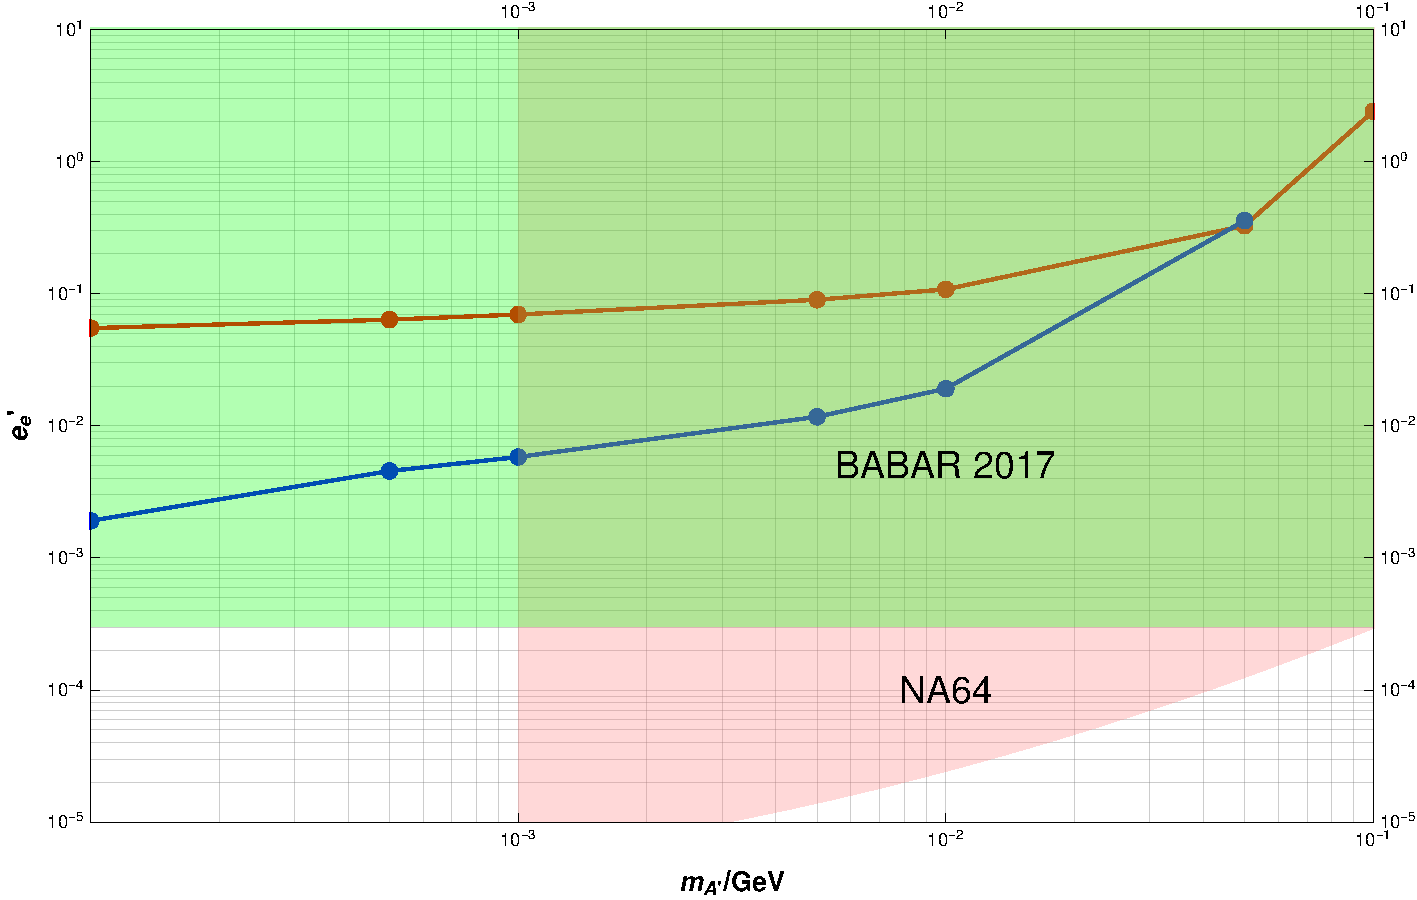
\includegraphics[width=0.8\textwidth]{imgs/combinedVector.pdf}
    \caption{95\% C.L. bounds on the vector mediator- electron coupling from the pion decay spectrum (red), the muon decay spectrum (blue), BABAR (green) and NA64 (pink)}
    \label{fg:PiMuCombinedVector}
\end{figure}

\begin{figure}[ht]
  \centering
    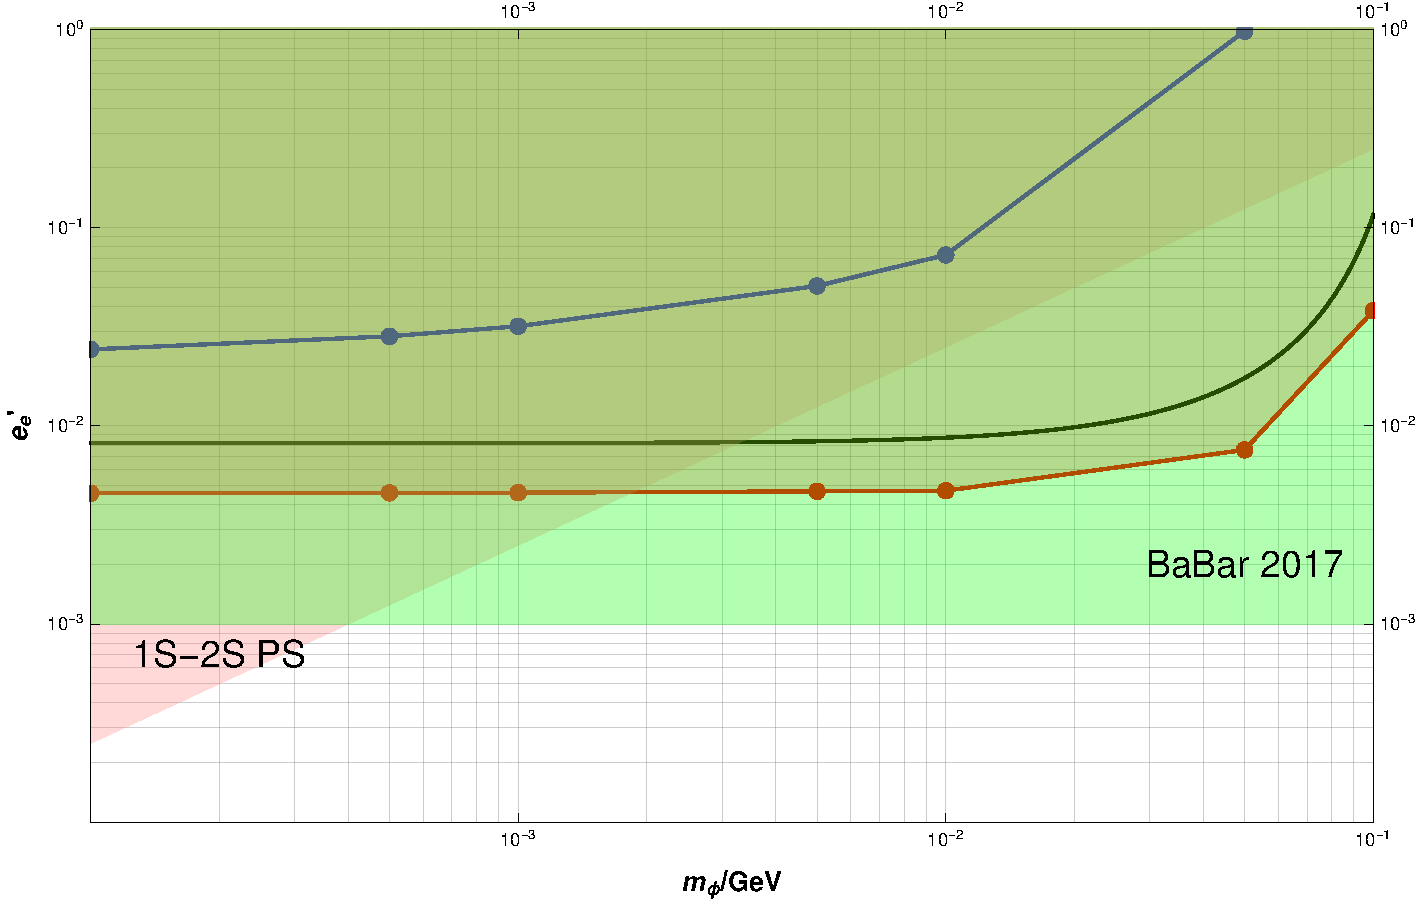
\includegraphics[width=0.8\textwidth]{imgs/combinedScalar.pdf}
    \caption{95\% C.L. bounds on the scalar mediator- electron coupling from pion decay spectrum (red), lepton universality in pion decays (smooth black line), the muon decay spectrum (blue), BABAR (green) and 1S-2S transition in positronium (pink)}
    \label{fg:PiMuCombinedScalar}
\end{figure}

Figure \ref{fg:PiMuCombinedVector} shows the combined results of both methods of constraining the parameter space of the vector mediator. In this case the analysis of the muon decay spectrum produces the stronger bounds. Despite not producing new bounds, future experimental results might produce competitive results using this method at least for light mediators.
Figure \ref{fg:PiMuCombinedScalar} shows the combined result for the scalar coupling to the electron. This time the muon results are considerably weaker than for the pion. 
\newpage
\chapter{Conclusion}
\label{ch:conclusion}

Here we have investigated models, that are not explicitly introduced to solve existing problems besides a possible explanation for dark matter. Nevertheless, some may at least be a subcomponent of these. The models here were for a scalar or vector mediator with masses between 0.1 to $\SI{100}{\mega \eV}$ and direct couplings only to leptons. That way these \emph{leptophilic} mediators don't leave strong signatures at high intensity proton accelerators and explain their null results for the search for dark matter. In the dark sector these mediators couple directly to the dark matter candidates $\chi$. If this coupling is large enough and the mediator decay to a $\bar{\chi}\chi$ pair is allowed, the main signatures in colliders is the missing energy which is somewhat more subtle than for example displaced vertices for visibly decaying mediators.

This thesis explored two novel ways of deriving limits on the parameter space.The first method introduced here, used the well known muon decay spectrum. The standard model decay spectrum is parametrised by Michel parameters to reflect potential additional interactions that might mediate the $\mu^+\rightarrow e^+ \nu_e \bar{\nu}_\mu$ decay besides the V-A interaction. These have been experimentally determined to great precision and yielded no significant deviation from the standard model. The main point made here, is that the only detected decay product is the positron, while the neutrinos escape detection. So processes with an additional particle coupled to any of the leptons, that also escapes detection, will be indistinguishable although it distorts the positron spectrum. This deformation was used to derive bounds on the coupling to the mediators. 

Scalar and vector mediators directly coupling to the electron result in bounds from the muon decay, that are weaker by more than one order of magnitude than missing energy searches by BABAR. Limits on the kinetic mixing parameter from BABAR or NA64 can be translated to bounds on the direct coupling between a vector mediator and the muon. Since this mixing only occurs at one loop, this translated bound is rather weak, even weaker than the derived bounds in this work. Additionally, bounds from neutrino trident production by CCFR are applicable for the vector to muon coupling model as well. The derived bounds from the muon decay are more than one order of magnitude weaker then the existing ones. Better bounds were only obtained for the scalar to muon coupling. Masses between $1$ and $\SI{20}{\mega \eV}$ and coupling constants between 0.04 and 0.2 were excluded by the muon decay, that were previously not excluded by existing experiments assuming mass hierarchical couplings $e_e'/e_\mu'=m_e/m_\mu$. The last model considered here was with gauged $L_{e-\mu}$ symmetry. Here the direct coupling to electrons result in strong existing constraints so that no new parameter space could be ruled out and the resulting bounds are weaker by more than one order of magnitude than the BABAR bounds.

Further constraints were derived from the standard model pion decay mode $\pi^+\rightarrow e^+ \nu_e$. As a two body decay the positron spectrum is a sharp peak that is experimentally broadened. The PIENU collaboration searched for additional peaks besides the standard model as a sign for heavy neutrinos. After subtracting the known standard model background, this can also be used to find bounds on the leptophilic mediators. Using a $\chi^2$ test to set 90\% and 95\% C.L. bounds, neither the vector nor the scalar coupling constraints to the electron could improve the known bounds from BABAR although the scalar results were parametrically around one order of magnitude stronger because this coupling removes the helicity suppression of this mode. Here an improvement of the experimental data by around one order might result in competitive bounds. 

Lastly the removal of the helicity suppression was used on its own to derive supplemental constraints on the scalar to electron coupling. Here a violation of apparent lepton universality would be enhanced by the scalar. Comparing the standard model prediction and experimental value of the test in pion decays sets constraints on the parameter space. Again the parameter space is already ruled out by BABAR. 

Future theoretical and experimental work continue to explore the parameter space of these models. Supplemental probes, like the ones presented above for the coupling between the scalar and muon or the scalar and electron after an improvement of the experimental sensitivity will continue to provide valuable insights. Especially since further improvement in the pion decay spectrum is well motivated by searches for heavy neutrinos, this method might become competitive. Any coupling to electrons can be investigated additionally in $e^+e^-$ colliders, since Belle II is currently running.
Couplings to the muon will continue to attract experimental effort since the $(g-2)_\mu$ anomaly is another problem waiting to be solved. If approved, the NA64-$\mu$ run or the $M^3$ experiment will reach unprecedented sensitivity to these scenarios.
All in all, the future will show exciting insights in the models considered above.
\newpage
\begin{appendices}
\chapter{Phase Space Integration}
If an unstable particle of mass $m_A$ decays to $N$ particles with four momenta $p_1,p_2...p_N\equiv\{p_f\}$
the differential decay rate is
\begin{equation}
d\Gamma = \frac{1}{2m_A}|\mathcal{M}(m_A\rightarrow\{p_f\})|^2d\Phi_{\text{lips}}(p_A\rightarrow\{p_f\})
\end{equation}
where the Lorentz-invariant phase space is defined as
\begin{equation}
d\Phi_{\text{lips}}(p_A\rightarrow\{p_f\}) \equiv \left(\prod_f\frac{d^3p_f}{(2\pi)^3}\frac{1}{2E_f}\right)(2\pi)^4\delta^{(4)}\left(p_A-\sum_i p_i\right).
\end{equation}
\paragraph{Two particle final-state}
In the case of only two final-state-particles with three momentum $\pm \vec{p}$ the phase space can be written as
\begin{equation}
d\Phi_{\text{lips}}(p_A\rightarrow\{p_1,p_2\})=\int \frac{\Omega_{\text{cm}}}{4\pi} \frac{1}{8\pi}\left(\frac{2|\vec{p}|}{E_\text{cm}}\right) 
\end{equation}
\paragraph{Three particle final-state}
The three particle case can still be solved relatively strait forward with some algebra and kinematical considerations. Though there is a ready to use recipe by Asatrian
\cite{Asatrian:2012tp}. Here one starts with "dimensionless" momenta $p'_i=p_i/m_A$ and works in the rest frame of $p_1$ and $p_3$ where $q' = p'_1+p'_2=(\sqrt{s_{13}},\vec{0})^T$.
The coordinate system can then be rotated such that the remaining two momenta are given by
\begin{align}
p'&=(E',|\vec{p'}|,0,0)\\
p'_3&=(E'_3,|\vec{p'_3}|\cos\theta,|\vec{p'_3}|\sin \theta,0).
\end{align}
With the mass fractions $x_i = m_i^2/m_A^2$ this may be expressed with
\begin{align*}
|\vec{p'}| &= \frac{1}{2\sqrt{s_{13}}}\sqrt{(1+x_2-s_{13})^2-4x_2}\\
|\vec{p'_3}|&=\frac{1}{2\sqrt{s_{13}}}\sqrt{(x_1+x_3-s_{13})^2-4x_1x_3}
\end{align*}
With
\begin{equation}
X\equiv -4|\vec{p'}||\vec{p'_3}|\cos\theta+1+2(x_1+x_3)-s_{13}-\frac{(1+s_{13}-x_2)(x_1-x_3)}{s_{13}}
\end{equation}
this can be used to express all combinations of momenta in scalar products in the matrix element by the following combinations:
\begin{align}
p'_i\cdot p'_i&= x_i\\
p'\cdot p'_1&=\frac{2(1+x_1+x_3)-x_2-X}{4}\\
p'\cdot p'_2&=\frac{1+x_2-s_{13}}{2}\\
p'\cdot p'_3&=\frac{-2(x_1+x_3)-x_2+2s_{13}+X}{4}\\
p'_1\cdot p'_2&=\frac{2+4x_3-x_2-2s_{13}-X}{4}\\
p'_1\cdot p'_3&=\frac{s_{13}-x_1-x_3}{2}\\
p'_2\cdot p'_3&= \frac{-x_2-4x_3+X}{4}.
\end{align}
The phase space integral can then be written as
\begin{equation}
d\Phi_{\text{lips}}(p_A\rightarrow\{p_1,p_2,p_3\})=\frac{m_A^2}{8(2\pi )^3}|\vec{p'}||\vec{p'_3}|d\cos\theta d s_{13}
\end{equation}
where $\cos\theta$ is to be integrated from $-1$ to $1$ and $s_{13}$ from $(\sqrt{x_1}+\sqrt{x_3})^2$ to $(1-\sqrt{x_2})^2$.
\paragraph{Four particle final-state for a polarised decay}
All in all there will be seven independent variables of integration. Asatrian gives also a recipe for this case. However, for this work, the differential decay rate of the decay in four particles is needed and Asatrian's method doesn't permit that.
Since there is virtually no hope in finding an analytical solution to all integrals encountered in this task, one might as well start in a direction that does allow relatively strait forward evaluation with numerical methods. 
To simplify matters lets work in the rest-frame of the decaying particle, adopt spherical coordinates $dp^3 \equiv d|p|d\Omega$ and specialise in the case, where particle three is massless.
Firstly, one may eliminate the overall energy-momentum conserving four delta distributions by replacing the three $p_4$ integrals using (writing the time component of $p_4$ as $E_4$ even though its not on shell)
\begin{equation}
\int\frac{d^3p_4}{2E_4}=\int d^4p_4\delta(p_4^2-m_4^2)\Theta(E_4)
\label{eq:AppOffShell}
\end{equation}
and carrying out the $dp_4$ integral:
\begin{align*}
\frac{1}{(2\pi)^8} \frac{d^3p_1}{2E_1}\frac{d^3p_2}{2E_2}\frac{d^3p_3}{2E_3}\delta\left((p_A-\sum_{i=1}^3p_i)^2-m_4^2\right)\Theta(m_A-\sum_{i=1}^3E_i)
\end{align*}
and changing the momenta to the energies
\begin{align*}
\frac{1}{2^3(2\pi)^8}\sqrt{E_1^2-m_1^2}\sqrt{E_2^2-m_2^2}E_3dE_1dE_2dE_3d\Omega_1d\Omega_2d\Omega_3\times \\ \delta\left((p_A-\sum_{i=1}^3p_i)^2-m_4^2\right)\Theta(m_A-\sum_{i=1}^3E_i).
\end{align*}
At this point it is advisable to adopt a specific coordinate frame where the z-axis is already fixed by the spin of the decaying particle:
\begin{align}
p_A&=(m_A,0,0,0)\\
p_1&=(E_1,\sqrt{E_1^2-m_1^2}\sin\theta_1,0,\sqrt{E_1^2-m_1^2}\cos\theta_1)\\
p_2&=(E_2,\sqrt{E_2^2-m_2^2}\sin\theta_2\cos\phi_2,\sqrt{E_2^2-m_2^2}\sin\theta_2\sin\phi_2,\sqrt{E_2^2-m_2^2}\cos\theta_2)\\
p_3&=(E_3,E_3\sin\theta_3\cos\phi_3,E_3\sin\theta_3\sin\phi_3,E_3^2\cos\theta_3)
\label{eq:momenta}
\end{align}
Now the phase-space weight and any momentum-scalar products are independent of $\phi_1$ so the integral can be carried out resulting in another factor of $2\pi$.

Lets now turn our attention to the delta distribution 
\begin{equation}
\int dE_3 \delta\left(\left(p_A-\sum_{i=1}^3p_i\right)^2-m_4^2\right)
\end{equation}
and use the $E_3$ integration to get rid of it:
\begin{align}
\begin{split}
=&\int dE_3 \delta(m_A^2+m_1^2+m_2^3-m_4^2-2m_A(E_1+E_2+E_3)\\
&-2E_1E_2+2\sqrt{E_1^2-m_1^2}\sqrt{E_2^2-m_2^2}(\sin\theta_1\sin\theta_2\cos\phi_2+\cos\theta_1\cos\theta_2))\\
&-2E_1E_3+2\sqrt{E_1^2-m_1^2}E_3(\sin\theta_1\sin\theta_3\cos\phi_3+\cos\theta_1\cos\theta_3))\\
&-2E_2E_3++2\sqrt{E_2^2-m_2^2}\sqrt{E_3^2-m_2^3}(\sin\theta_2\cos\phi_2\sin\theta_3\cos\phi_3\\
&+\sin\theta_2\sin\phi_2\sin\theta_3\sin\phi_3+\cos\theta_2\cos\theta_3))\\
=&\lvert-2\sqrt{E_1^2-m_1^2}(\sin\phi_3\sin\theta_1\sin\theta_3+\cos\theta_1\cos\theta_3)+2E_1-2\sqrt{E_2^2-m_2^2}\\&\cdot(\sin\theta_2\sin\theta_3\cos(\phi_2-\phi_3)+\cos\theta_2\cos\theta_3)+2E_2-2m_a\rvert^{-1}\theta(\widetilde{E}_3)\\
\equiv&|\alpha|\theta(\widetilde{E}_3)
\end{split}
\end{align}
with
\begin{align*}
\widetilde{E}_3=&\alpha\Bigl{(}2\sqrt{E_1^2-m_1^2}\sqrt{E_2^2-m_2^2}(\sin\phi_2\sin\theta_1\sin\theta_2+\cos\theta_1\cos\theta_2)\\&-2E_1E_2+2E_1m_A+2E_2m_A-m_A^2-m_1^2-m_2^2\Bigr{)}
\end{align*}
where the Heaviside function comes from using equation \ref{eq:AppOffShell} to carry out the integration off-shell to ensure that the argument of the delta distribution has a root on the integration interval.

\chapter{Additional Bounds on Chiral Couplings}
Here additional bounds on coupling to the leptons that depend on the chirality are presented. These can be introduced by terms like
\begin{align}
\mathcal{L} &\supset \sum_{l=e,\mu,\tau}g'_{l,L}\cdot\bar{L}_l\gamma_\mu A'^\mu L_l+\sum_{l=e,\mu,\tau}g'_{l,R}\cdot\bar{e}_{lR}\gamma_\mu A'^\mu e_{lR}\\
&=\sum_{l=e,\mu,\tau} g'_{l,L}\left(\bar{l}\gamma^\mu A'_\mu P_L l+\bar{\nu}_l\gamma^\mu A'_\mu \nu_l\right)+\sum_{l=e,\mu,\tau} g'_{l,R}\bar{l}\gamma^\mu A'_\mu P_R l
\end{align}
Competing bounds will not be explicitly stated, because these models are not treated separately in the literature, even though some may be extrapolated. 
\begin{figure}[H]
  \centering
    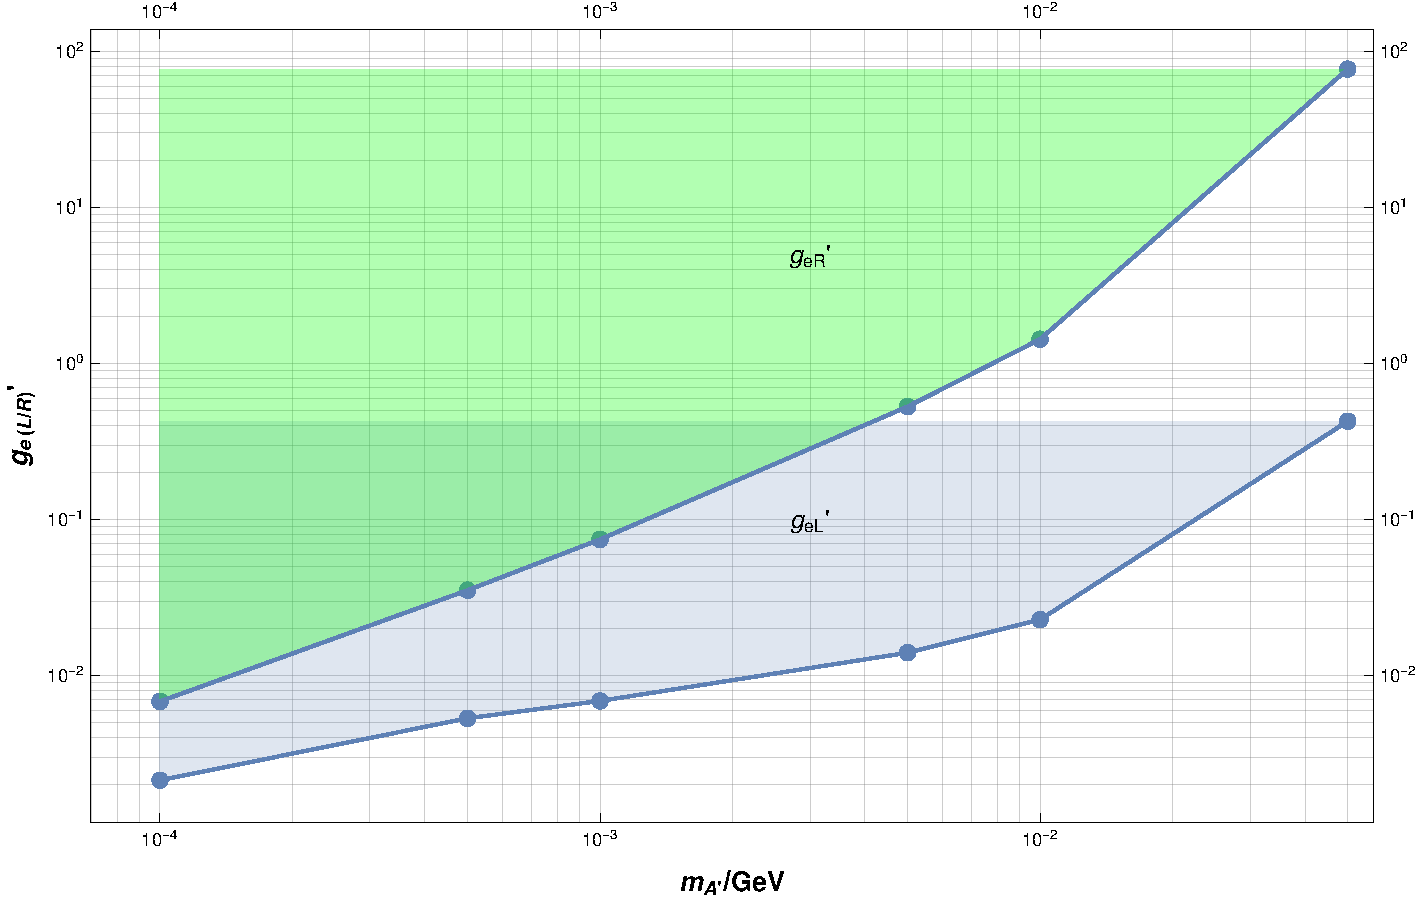
\includegraphics[width=\textwidth]{imgs/BoundERL}
    \caption{Bound on the left/right exclusive couplings to the electron}
    \label{fg:ERLBound}
\end{figure}
\begin{figure}[H]
  \centering
    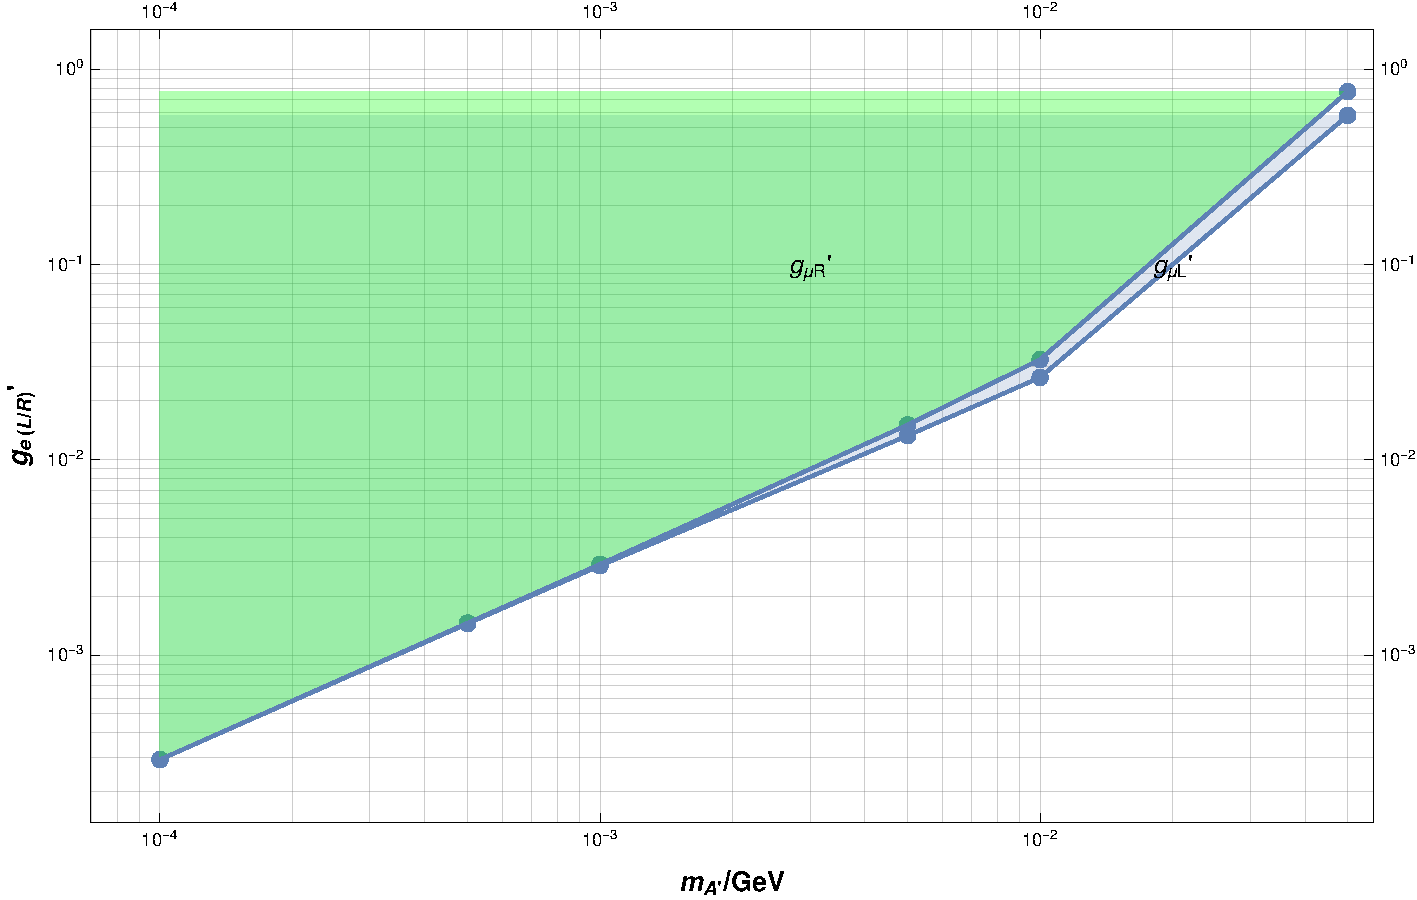
\includegraphics[width=\textwidth]{imgs/BoundMRL}
    \caption{Bound on the left/right exclusive couplings to the muon}
    \label{fg:MRLBound}
\end{figure}
\end{appendices}
\nocite{*}
%\bibliographystyle{h-physrev}
\addcontentsline{toc}{chapter}{Bibliography}
\bibliographystyle{JHEP}
\bibliography{bibliography.bib}
\end{document}